% ===================== main.tex (FULL) =====================
\documentclass[12pt,a4paper]{article}

% ================== GÓI TIẾNG VIỆT & CƠ BẢN ==================
% Thứ tự ổn định cho pdfLaTeX + vntex
\usepackage[utf8]{inputenc}
\usepackage[utf8]{vntex}
\usepackage[english,vietnamese]{babel}

% ================== NÉ LỖI SPLIT BOX / GLUE ==================
% Giảm việc TeX ép co giãn chiều dọc khi ngắt trang
\raggedbottom

% ================== FONT ==================
% Latin Modern để ổn định hơn khi dùng T5
\usepackage{lmodern}
\renewcommand{\ttdefault}{lmtt}

% ================== CỘT BẢNG RAGGEDRIGHT ==================
\usepackage{array}
\newcolumntype{L}[1]{>{\raggedright\arraybackslash}p{#1}}
\newcolumntype{Y}{>{\raggedright\arraybackslash}X}

% ================== GÓI CƠ BẢN ==================
\usepackage{blindtext}
\usepackage{float}
\usepackage{pdfpages}
\usepackage{longtable}

\definecolor{codebg}{RGB}{245,245,245}
\definecolor{codeframe}{RGB}{200,200,200}
\definecolor{codekeyword}{RGB}{0,0,120}
\definecolor{codestring}{RGB}{120,0,0}
\definecolor{codecomment}{RGB}{0,96,0}

% ================== GÓI BỔ TRỢ ==================
\usepackage{a4wide,amssymb,epsfig,latexsym,multicol,hhline,fancyhdr}
\usepackage[dvipsnames]{xcolor}
\usepackage[framemethod=tikz]{mdframed}
\usepackage{lastpage}
\usepackage[lined,boxed,commentsnumbered]{algorithm2e}
\usepackage{enumerate}
\usepackage{alltt}
\usepackage{graphicx}
\usepackage{tabularx}
\usepackage{booktabs}
\usepackage{lipsum}
\usepackage{pdflscape}
\usepackage{multirow}
\usepackage{multicol}
\usepackage{rotating}
\usepackage{subcaption}
\usepackage{sectsty}
\usepackage{geometry}
\usepackage{setspace}
\usepackage{amsmath}
\usepackage{enumitem}
\usepackage{tikz}
\usepackage{indentfirst}
\usetikzlibrary{arrows,snakes,backgrounds,calc}
\usepackage{colortbl}
\usepackage{makecell}
\usepackage{listings}

% ================== BIBLIOGRAPHY ==================
\usepackage[
    backend=biber,
    style=numeric,
    sorting=none,
    language=english
]{biblatex}
\addbibresource{refs.bib}

% ================== LISTINGS ==================
\lstdefinelanguage{json}{
  morestring=[b]",
  morecomment=[l]{//},
  morecomment=[s]{/*}{*/},
  morekeywords={true,false,null}
}
\lstdefinestyle{report}{
  backgroundcolor=\color{codebg},
  frame=single,
  rulecolor=\color{codeframe},
  basicstyle=\ttfamily\small,
  keywordstyle=\color{codekeyword}\bfseries,
  stringstyle=\color{codestring},
  commentstyle=\color{codecomment}\itshape,
  numbers=left,
  numberstyle=\tiny\color{gray},
  stepnumber=1,
  numbersep=8pt,
  breaklines=true,
  breakatwhitespace=true,
  showstringspaces=false,
  tabsize=2,
  captionpos=b,
  xleftmargin=1em,
  xrightmargin=1em
}
\lstset{style=report}

% ================== HYPERREF ==================
\usepackage[unicode,hypertexnames=false]{hyperref}
\hypersetup{
    hidelinks,
    colorlinks=false
}

% ================== LỀ TRANG ==================
\geometry{
    a4paper,
    left=20mm,
    right=20mm,
    top=20mm,
    bottom=25mm
}

% ================== DÒNG CÁCH ==================
\onehalfspacing

% ================== HEADER / FOOTER ==================
\setlength{\headheight}{40pt}
\pagestyle{fancy}
\fancyhead{}
\fancyfoot{}

% KHÔNG dùng \ttfamily cho tiếng Việt ở footer
\fancyfoot[L]{\scriptsize \sffamily Khoa Khoa Học và Kỹ Thuật Máy Tính}
\fancyfoot[R]{\scriptsize \sffamily Page {\thepage}/\pageref{LastPage}}

\renewcommand{\headrulewidth}{0pt}
\renewcommand{\footrulewidth}{0.3pt}

% ================== KHÁC ==================
\renewcommand{\contentsname}{Mục lục}

%%%%%%%%%%%%%%%%%%%%%%%%%%%%%%%%%%%%%%%%%%%%%%%%%%%%%%%%%%%%%%%%%%%%%%%%%
\begin{document}

% ===================== TRANG BÌA (có thông tin hội đồng) =====================
\begin{titlepage}
\thispagestyle{empty}

\begin{tikzpicture}[remember picture, overlay]
  \draw[line width = 4pt] ($(current page.north west) + (0.4in,-0.5in)$)
        rectangle ($(current page.south east) + (-0.4in,0.5in)$);
  \draw[line width=1.5pt]
        ($(current page.north west) + (0.45in,-0.55in)$)
        rectangle
        ($(current page.south east) + (-0.45in,0.55in)$);
\end{tikzpicture}

\vspace{-2cm}
\begin{center}
    \fontsize{14}{16}\selectfont\textbf{ĐẠI HỌC QUỐC GIA TP. HỒ CHÍ MINH}\\[0.2cm]
    \fontsize{14}{16}\selectfont\textbf{TRƯỜNG ĐẠI HỌC BÁCH KHOA}\\[0.2cm]
    \fontsize{14}{16}\selectfont\textbf{KHOA KHOA HỌC VÀ KỸ THUẬT MÁY TÍNH}
\end{center}

\vspace{0.4cm}

\begin{figure}[H]
\centering
\includegraphics[width=5cm]{Images/hcmut.png}
\end{figure}

\vspace{0.4cm}

\begin{center}
    \fontsize{16}{18}\selectfont\textbf{ĐỒ ÁN CHUYÊN NGÀNH}\\[0.2cm]
    \fontsize{16}{18}\selectfont\textbf{BÁO CÁO}
\end{center}

\vspace{0.8cm}

\begin{center}
    \setstretch{1.6}
    {\fontsize{18}{20}\selectfont\textbf{PHÁT TRIỂN HỆ THỐNG GAME ONLINE}}\\[0.1cm]
    {\fontsize{18}{20}\selectfont\textbf{NHẬP VAI HÀNH ĐỘNG NHIỀU NGƯỜI CHƠI}}\\[0.3cm]
    {\fontsize{14}{16}\selectfont\textbf{“FORTRESS OF THE FALLEN”}}\\[0.6cm]
    {\fontsize{14}{16}\selectfont Ngành: Khoa học Máy tính}\\[0.2cm]
    {\fontsize{12}{14}\selectfont Học kỳ 1 năm học 2025–2026 (HK251)}
\end{center}

\vspace{1cm}

\begin{center}
\fontsize{13}{15}\selectfont
\renewcommand{\arraystretch}{1.4}

% Dòng giảng viên
\begin{tabular}{@{}ll@{}}
    \textbf{Giảng viên hướng dẫn:} & ThS. Vương Bá Thịnh \\
\end{tabular}

\vspace{0.5cm}

% Bảng sinh viên 2 cột
\begin{tabular}{@{}l c@{}}
    \textbf{Sinh viên thực hiện} & \textbf{MSSV} \\[0.2cm]
    Hà Thái Toàn      & 2213524 \\
    Trần Minh Khang   & 2211472 \\
\end{tabular}


\end{center}

\vfill

\begin{center}
    \fontsize{13}{15}\selectfont TP. Hồ Chí Minh, năm 2025
\end{center}

\end{titlepage}


% Phần đầu: đánh số trang kiểu roman (trang bìa để empty nên không hiển thị số)
\clearpage
\pagenumbering{roman}

% ===================== LỜI CẢM ƠN =====================
% ===================== Content/acknowledgements.tex =====================
\section*{Lời cảm ơn}
\addcontentsline{toc}{section}{Lời cảm ơn}

Trong quá trình thực hiện đồ án ``Phát triển hệ thống game online nhập vai hành động nhiều người chơi \textit{Fortress of the Fallen}'', nhóm đã nhận được sự hỗ trợ, hướng dẫn và tạo điều kiện từ nhiều cá nhân và tập thể. Với tinh thần trân trọng, nhóm xin gửi lời cảm ơn chân thành đến những người đã đồng hành và đóng góp để nhóm có thể hoàn thành đồ án cũng như báo cáo theo đúng mục tiêu và phạm vi đề ra.

Trước hết, nhóm xin bày tỏ lòng biết ơn sâu sắc đến \textbf{ThS. Vương Bá Thịnh} --- giảng viên hướng dẫn trực tiếp --- người đã dành nhiều thời gian theo sát tiến độ, định hướng phương pháp tiếp cận và liên tục góp ý trong từng giai đoạn. Từ việc chốt phạm vi bài toán, thống nhất mô hình client--server, tổ chức mô-đun backend theo hướng rõ ràng, cho đến việc hoàn thiện thiết kế dữ liệu và luồng giao tiếp REST/WebSocket, những nhận xét của thầy đã giúp nhóm tránh được các sai lệch phổ biến khi phát triển một hệ thống game online. Không chỉ hỗ trợ về mặt kỹ thuật, thầy còn góp ý cách trình bày báo cáo theo hướng chặt chẽ, có luận điểm và có dẫn chứng, giúp nhóm cải thiện đáng kể chất lượng nội dung và tính nhất quán giữa các chương.

Nhóm xin chân thành cảm ơn \textbf{quý thầy/cô trong Khoa Khoa học và Kỹ thuật Máy tính} đã giảng dạy và trang bị nền tảng kiến thức xuyên suốt quá trình học tập. Các học phần liên quan đến công nghệ phần mềm, cơ sở dữ liệu, mạng máy tính, hệ thống phân tán, cũng như các kỹ năng phân tích và thiết kế hệ thống đã tạo tiền đề quan trọng để nhóm có thể tiếp cận đề tài theo hướng có phương pháp. Bên cạnh đó, môi trường học tập của Khoa giúp nhóm rèn luyện tư duy kỷ luật, cách làm việc theo quy trình, và ý thức về chất lượng sản phẩm, đặc biệt quan trọng với những đề tài có tính tích hợp cao giữa gameplay, backend, dữ liệu và vận hành.

Nhóm cũng xin gửi lời cảm ơn đến \textbf{Hội đồng chấm bảo vệ} đã dành thời gian đọc, đánh giá và góp ý cho đồ án. Các nhận xét phản biện và gợi ý cải thiện là cơ sở để nhóm nhìn nhận rõ hơn những điểm còn hạn chế về kiến trúc, dữ liệu và trải nghiệm người dùng, đồng thời định hướng các hạng mục cần ưu tiên trong các giai đoạn phát triển tiếp theo. Nhóm xin tiếp thu nghiêm túc các góp ý và sẽ chủ động điều chỉnh để hoàn thiện sản phẩm ở mức tốt hơn.

Trong suốt quá trình triển khai, nhóm cũng nhận được nhiều hỗ trợ từ \textbf{bạn bè, các anh/chị khóa trên và các nhóm đồ án khác} thông qua việc trao đổi kinh nghiệm và chia sẻ tài liệu tham khảo. Những trao đổi về cách tổ chức mã nguồn, cách quản lý tài nguyên (asset), cách thiết kế cấu hình theo hướng data-driven, cũng như các lưu ý khi kiểm thử luồng nghiệp vụ và xử lý lỗi thực tế đã giúp nhóm rút ngắn đáng kể thời gian thử--sai. Đây là nguồn tham khảo hữu ích để nhóm cân bằng giữa mục tiêu kỹ thuật và giới hạn thời gian của một đồ án học thuật.

Cuối cùng, nhóm xin gửi lời cảm ơn sâu sắc đến \textbf{gia đình} đã luôn động viên, tạo điều kiện và hỗ trợ tinh thần để nhóm có thể tập trung thực hiện đồ án trong giai đoạn cao điểm. Sự cảm thông và đồng hành của gia đình là động lực quan trọng để nhóm duy trì kỷ luật làm việc, hoàn thành các mốc tiến độ và vượt qua áp lực về thời gian.

Nhóm ý thức rằng, dù đã nỗ lực hoàn thiện trong phạm vi cho phép, báo cáo và sản phẩm hiện thực vẫn có thể còn thiếu sót do giới hạn nguồn lực và thời lượng thực hiện. Nhóm kính mong tiếp tục nhận được sự góp ý từ quý thầy/cô để có thể hoàn thiện hơn trong các bước phát triển kế tiếp. Nhóm xin trân trọng cảm ơn.

\vspace{0.8cm}
\begin{flushright}
TP. Hồ Chí Minh, năm 2025
\end{flushright}

\clearpage

% ===================== LỜI CAM ĐOAN =====================
% ===================== Content/protestation.tex (EXPANDED, NO ITEMIZE) =====================
\section*{Lời cam đoan}
\addcontentsline{toc}{section}{Lời cam đoan}

Chúng tôi xin cam đoan rằng báo cáo đồ án ``Phát triển hệ thống game online nhập vai hành động nhiều người chơi \textit{Fortress of the Fallen}'' là kết quả của quá trình nghiên cứu, phân tích, thiết kế và hiện thực do nhóm tự thực hiện dưới sự hướng dẫn của giảng viên hướng dẫn. Toàn bộ nội dung được trình bày trong báo cáo phản ánh trung thực các công việc mà nhóm đã thực hiện trong phạm vi đồ án, bao gồm việc xác định mục tiêu và phạm vi hệ thống, phân tích yêu cầu, thiết kế kiến trúc tổng thể client--server, thiết kế mô-đun backend, thiết kế dữ liệu và giao tiếp, cũng như mô tả hiện thực, kiểm thử và đánh giá kết quả.

Chúng tôi cam kết rằng các phần nội dung mang tính tham khảo, kế thừa hoặc tổng hợp từ các nguồn tài liệu bên ngoài (sách, bài báo, tài liệu kỹ thuật, tài liệu hướng dẫn, hình minh hoạ tham khảo, và các nguồn công khai khác) đều được trích dẫn hoặc ghi nguồn phù hợp theo quy định của báo cáo. Các ý tưởng và cách tiếp cận được tham khảo chỉ đóng vai trò làm cơ sở lý thuyết hoặc định hướng triển khai, còn việc lựa chọn giải pháp, điều chỉnh theo phạm vi đề tài, tổ chức cấu trúc hệ thống, thiết kế dữ liệu, quy ước API, và hiện thực các chức năng cụ thể là do nhóm tự xây dựng. Chúng tôi không sao chép nguyên văn hoặc sử dụng sản phẩm nghiên cứu/hiện thực của bất kỳ cá nhân hay tổ chức nào như là kết quả của nhóm khi chưa được ghi nhận nguồn trích dẫn đúng quy định.

Chúng tôi cũng cam kết rằng các số liệu, bảng biểu, sơ đồ, hình ảnh và nội dung mô tả trong báo cáo được sử dụng nhằm mục đích học thuật và phục vụ việc trình bày kết quả nghiên cứu. Những nội dung này được thể hiện theo đúng hiểu biết và kết quả thực tế của nhóm trong quá trình thực hiện. Các đánh giá về mức độ hoàn thiện, ưu điểm, hạn chế và hướng phát triển tiếp theo được trình bày khách quan theo phạm vi đã triển khai; nhóm không cố tình làm sai lệch kết quả, không thổi phồng năng lực hệ thống, và không đưa ra những nhận định vượt quá bằng chứng/khả năng kiểm chứng trong đồ án.

Chúng tôi hiểu rằng tính trung thực và chuẩn mực học thuật là yêu cầu bắt buộc đối với một báo cáo đồ án. Do đó, chúng tôi xin hoàn toàn chịu trách nhiệm trước Khoa và Trường về nội dung của báo cáo này. Trong trường hợp phát hiện có sai sót liên quan đến trích dẫn, bản quyền hoặc tính chính xác của thông tin, nhóm cam kết sẽ nghiêm túc tiếp thu, chỉnh sửa và bổ sung theo yêu cầu của giảng viên hướng dẫn và Hội đồng, đồng thời chịu mọi hình thức xử lý (nếu có) theo quy định hiện hành.

Bằng lời cam đoan này, chúng tôi xác nhận rằng các nội dung trong báo cáo là trung thực, có nguồn gốc rõ ràng và được thực hiện đúng tinh thần học thuật.

\vspace{1.0cm}
\begin{flushright}
TP. Hồ Chí Minh, năm 2025
\end{flushright}

\clearpage

% ===================== TÓM TẮT =====================
% ===================== Content/abstract.tex =====================
\section*{Tóm tắt}
\addcontentsline{toc}{section}{Tóm tắt}

Đồ án tập trung phát triển một hệ thống game online nhập vai hành động nhiều người chơi có tên \textit{Fortress of the Fallen}. Mục tiêu của đề tài là xây dựng nền tảng client--server có khả năng vận hành ổn định cho các chức năng cốt lõi: xác thực người dùng, quản lý profile/nhân vật, quản lý túi đồ và trang bị, hệ thống kỹ năng, lưu trữ tiến trình người chơi và các mô-đun gameplay mở rộng như đảo cá nhân, NPC và gacha.

Hệ thống được tổ chức theo mô hình server-authoritative nhằm đảm bảo tính nhất quán dữ liệu và giảm rủi ro gian lận. Client (Unity) giao tiếp với backend (NestJS) thông qua REST cho các tác vụ meta (đăng nhập, tải dữ liệu, quản lý nhân vật) và WebSocket cho các tương tác yêu cầu thời gian thực. Cơ sở dữ liệu MongoDB lưu trữ dữ liệu tiến trình, trong khi dữ liệu cấu hình gameplay được quản trị theo hướng data-driven thông qua quy trình: soạn thảo trên Google Sheets, xuất TSV, import vào database và nạp vào Config Manager khi hệ thống khởi động.

Kết quả đồ án là một kiến trúc mô-đun rõ ràng, có khả năng mở rộng theo từng phân hệ và hỗ trợ kiểm thử tích hợp dựa trên các luồng nghiệp vụ chính.

\vspace{0.3cm}
\noindent\textbf{Từ khóa:} game online, Action RPG, client--server, server-authoritative, NestJS, MongoDB, WebSocket, data-driven configuration.

\clearpage

% ===================== DANH MỤC THUẬT NGỮ =====================
\section*{Danh mục thuật ngữ}
\addcontentsline{toc}{section}{Danh mục thuật ngữ}

\noindent
Bảng dưới đây liệt kê các thuật ngữ và viết tắt thường được sử dụng trong báo cáo, đặc biệt liên quan tới phát triển game online, kiến trúc client--server, hệ thống AI NPC và cơ sở dữ liệu. Các thuật ngữ này sẽ được dùng xuyên suốt các chương sau.

\vspace{0.5cm}

\renewcommand{\arraystretch}{1.3}

% Điều chỉnh khoảng cách trên/dưới longtable nếu muốn
\setlength{\LTpre}{0pt}
\setlength{\LTpost}{0pt}

\begin{longtable}{|p{3cm}|p{4cm}|p{8cm}|}
\hline
\textbf{Thuật ngữ} & \textbf{Tên đầy đủ} & \textbf{Giải thích} \\
\hline
\endfirsthead

\hline
\textbf{Thuật ngữ} & \textbf{Tên đầy đủ} & \textbf{Giải thích} \\
\hline
\endhead

\hline
\multicolumn{3}{r|}{(còn tiếp trang sau)}\\
\hline
\endfoot

\hline
\endlastfoot

% ====== NHÓM 1: GAME & GAMEPLAY =======================================
\multicolumn{3}{|l|}{\textbf{Nhóm thuật ngữ về game và gameplay}} \\ \hline

RPG & Role-Playing Game &
Game nhập vai, trong đó người chơi điều khiển một hoặc nhiều nhân vật, phát triển sức mạnh thông qua hệ thống level, chỉ số, kỹ năng, trang bị và cốt truyện. \\ \hline

Action RPG & Action Role-Playing Game &
Game nhập vai hành động, chiến đấu diễn ra theo thời gian thực (real-time), người chơi điều khiển trực tiếp nhân vật (tấn công, né, dùng kỹ năng) thay vì theo lượt (turn-based). \\ \hline

PvP & Player vs Player &
Chế độ người chơi chiến đấu trực tiếp với người chơi khác. Yêu cầu đồng bộ trạng thái nhanh, cơ chế xử lý độ trễ và chống gian lận mạnh. \\ \hline

PvE & Player vs Environment &
Chế độ người chơi đối đầu với quái, boss hoặc môi trường do hệ thống điều khiển. Trong \textit{Fortress of the Fallen}, phần lớn nội dung dungeon, tháp, đảo cá nhân ban đầu thiên về PvE. \\ \hline

Boss & Boss &
Kẻ địch đặc biệt có chỉ số cao, cơ chế tấn công phức tạp, thường là trọng tâm của một dungeon hoặc tầng tháp. \\ \hline

Dungeon & Dungeon &
Khu vực (thường là instance riêng) tập trung chiến đấu, vượt thử thách. Trong đề tài, dungeon có thể là các tầng Tinh Hà Trung Tâm hoặc các khu vực phụ. \\ \hline

Hitbox & Hitbox &
Vùng hình học trong game đại diện cho phạm vi đòn tấn công có hiệu lực (ví dụ: vùng chém của kiếm, vùng nổ của kỹ năng). \\ \hline

Hurtbox & Hurtbox &
Vùng hình học đại diện cho khu vực trên nhân vật có thể nhận sát thương. Va chạm giữa hitbox và hurtbox thường được sử dụng để quyết định trúng đòn. \\ \hline

Cooldown (CD) & Cooldown &
Thời gian chờ sau khi sử dụng kỹ năng trước khi kỹ năng đó có thể được sử dụng lại. \\ \hline

Animation & Animation &
Chuỗi hình ảnh mô phỏng chuyển động (chạy, tấn công, né, trúng đòn...). Trong Action RPG, animation gắn chặt với gameplay. \\ \hline

% ====== NHÓM 2: MULTIPLAYER & NETWORKING ===============================
\multicolumn{3}{|l|}{\textbf{Nhóm thuật ngữ về multiplayer và networking}} \\ \hline

Multiplayer & Multiplayer &
Hình thức chơi nhiều người, cho phép nhiều người chơi cùng tồn tại và tương tác trong một thế giới game chung (ví dụ: cùng ở một đảo, dungeon, tầng tháp). \\ \hline

Real-time & Real-time &
Thời gian thực: hệ thống xử lý và phản hồi gần như ngay lập tức theo input của người chơi. \\ \hline

Latency & Network Latency &
Độ trễ mạng, là thời gian gói tin đi từ client tới server. Thường đo bằng mili-giây (ms). \\ \hline

Tick rate & Server Tick Rate &
Số lần server cập nhật trạng thái game trong một giây (ví dụ: 20~tick/s, 30~tick/s). \\ \hline

Snapshot & State Snapshot &
Bản “ảnh chụp” trạng thái game tại một thời điểm (vị trí nhân vật, HP, trạng thái kỹ năng...), được server gửi cho client để đồng bộ. \\ \hline

Client-side Prediction & Client-side Prediction &
Kỹ thuật client dự đoán trước kết quả chuyển động, hành động dựa trên input người chơi, nhằm giảm cảm giác trễ. \\ \hline

Reconciliation & Reconciliation &
Quá trình đồng bộ lại trên client: so sánh trạng thái dự đoán với trạng thái do server gửi về và điều chỉnh để khớp. \\ \hline

Server Authoritative & Server Authoritative Model &
Mô hình trong đó server nắm quyền quyết định cuối cùng về logic game (di chuyển hợp lệ, sát thương, kết quả combat). \\ \hline

WebSocket & WebSocket &
Giao thức truyền thông hai chiều trên nền TCP, cho phép client và server giữ kết nối lâu dài và gửi/nhận dữ liệu thời gian thực. \\ \hline

Instance & Instance &
Phiên bản riêng biệt của một khu vực game (ví dụ: một dungeon hoặc một tầng tháp tạo riêng cho một nhóm người chơi). \\ \hline

Zone / Shard & Zone / Shard &
Khu vực logic trong thế giới game, dùng để chia tải hoặc phân vùng nội dung. \\ \hline

Interest Management & Interest Management &
Kỹ thuật lọc và chỉ gửi dữ liệu cần thiết cho mỗi client để giảm băng thông và tải xử lý. \\ \hline

% ====== NHÓM 3, 4, 5: bạn copy các dòng còn lại từ bảng cũ vào đây, giữ đúng cấu trúc:
%  - mỗi dòng kết thúc bằng \\ \hline
%  - mỗi tiêu đề nhóm: \multicolumn{3}{|l|}{\textbf{Tên nhóm}} \\ \hline

\end{longtable}

\clearpage

% ===================== TOC, LOF, LOT =====================
\begin{singlespace}
\tableofcontents
\end{singlespace}
\clearpage

\begin{singlespace}
\listoffigures
\end{singlespace}
\clearpage

\begin{singlespace}
\listoftables
\end{singlespace}
\clearpage

% ===================== NỘI DUNG CHÍNH =====================
\pagenumbering{arabic}

% (Tuỳ chọn) Reset bộ đếm trước nội dung chính
\setcounter{table}{0}
\setcounter{figure}{0}
\setcounter{section}{0}

\section{Giới thiệu}

\subsection{Động lực}

Trong những năm gần đây, thị trường game trực tuyến tiếp tục tăng trưởng và xu hướng người chơi chuyển dịch mạnh sang các sản phẩm có tính tương tác và cập nhật liên tục\cite{newzoo-report}. Đặc biệt, nhóm trò chơi nhập vai hành động trực tuyến (Online Action RPG) đặt ra yêu cầu cao cả về trải nghiệm thời gian thực (real-time) lẫn tiến trình dài hạn (meta-progression). Người chơi kỳ vọng hệ thống vận hành ổn định, đồng bộ trạng thái mượt mà, phản hồi nhanh và đảm bảo tính nhất quán khi tương tác với nhiều phân hệ gameplay trong cùng một tài khoản.

Để đáp ứng các kỳ vọng đó, hệ thống phía server không chỉ xử lý xác thực và lưu trữ dữ liệu, mà còn phải đảm nhiệm các bài toán đặc thù của game online như:
\begin{itemize}
    \item Quản lý phiên chơi và xử lý nhiều kết nối đồng thời.
    \item Đồng bộ trạng thái theo mô hình phù hợp để giảm sai lệch giữa client và server, đồng thời hạn chế gian lận ở mức kiến trúc\cite{moriarty-networked}.
    \item Thiết kế dữ liệu tiến trình người chơi (profile/\allowbreak character/\allowbreak inventory/\allowbreak island/\allowbreak npc) sao cho có thể mở rộng và truy vết.
    \item Tổ chức nhiều phân hệ nghiệp vụ (combat, progression, gacha, base-building, admin) trong một kiến trúc nhất quán, giảm phụ thuộc chéo và thuận lợi bảo trì\cite{gregory-engine}.
\end{itemize}

Ngoài ra, một thách thức quan trọng trong thiết kế game là quản trị \textbf{game configuration} (dữ liệu tĩnh) như định nghĩa vật phẩm, công trình, tham số cân bằng, bảng tỉ lệ và cấu hình sự kiện. Nếu cấu hình bị gắn chặt vào mã nguồn, việc điều chỉnh nội dung và cân bằng sẽ phụ thuộc vào chu kỳ build và phát hành. Do đó, hướng tiếp cận \textit{data-driven} thường được áp dụng để tách cấu hình khỏi code, giúp quy trình cập nhật linh hoạt hơn và giảm rủi ro ``hard-code'' tham số\cite{adams-game-design,schell-art}.

Trong bối cảnh đó, đề tài \textit{Fortress of the Fallen} được thực hiện với trọng tâm là phân tích và thiết kế hệ thống cho một game Online Action RPG. Báo cáo hướng đến mô tả đầy đủ các phân hệ cốt lõi ở mức đồ án chuyên ngành, làm nền tảng cho các giai đoạn hiện thực tiếp theo.

\subsection{Mục tiêu}

Mục tiêu tổng quát của đề tài là xây dựng \textbf{bản thiết kế hệ thống} cho trò chơi Online Action RPG \textit{Fortress of the Fallen}, bao gồm kiến trúc, mô hình dữ liệu, luồng nghiệp vụ và hợp đồng giao tiếp giữa các thành phần.

Trong \textbf{giai đoạn 1}, đề tài tập trung vào các mục tiêu cụ thể:
\begin{itemize}
    \item Xác định phạm vi và mô tả tập tính năng ở mức hệ thống theo các phân hệ: Authentication \& Profile, Combat \& Gameplay, Character Progression, Recruitment (Gacha), Personal Island, và Administration.
    \item Phân tích yêu cầu chức năng, phi chức năng và yêu cầu dữ liệu; làm rõ ranh giới giữa dữ liệu tiến trình người chơi và dữ liệu cấu hình tĩnh.
    \item Thiết kế kiến trúc triển khai tổng thể theo mô hình client--server, bao gồm các thành phần backend và hạ tầng dữ liệu; xác định cơ chế giao tiếp phù hợp cho tác vụ request--response và real-time\cite{moriarty-networked,gregory-engine}.
    \item Thiết kế mô hình dữ liệu mức logic cho các thực thể chính: user, profile, session, character, inventory, island, npc và quan hệ giữa chúng, phục vụ truy vấn và mở rộng tính năng về sau.
    \item Thiết kế pipeline quản trị \textbf{game configuration (tĩnh)} theo hướng data-driven:
    \begin{center}
        Google Sheets $\rightarrow$ TSV $\rightarrow$ Import vào DB (collections cấu hình) $\rightarrow$ Load vào \textit{Config Manager} khi khởi động.
    \end{center}
    Pipeline này \textbf{chỉ áp dụng cho game configuration} \\
    Ví dụ: CONFIG\_ITEM, CONFIG\_SKILL, CONFIG\_ENEMY và các bảng cấu hình mở rộng, không áp dụng cho dữ liệu tiến trình người chơi.
\end{itemize}

\subsection{Phạm vi}

\subsubsection{Phạm vi trong giai đoạn 1}

Giai đoạn 1 tập trung hoàn toàn vào \textbf{phân tích và thiết kế}, bao gồm:

\begin{itemize}
    \item \textbf{Thiết kế phân hệ và luồng nghiệp vụ:}
    mô tả actors, use case, luồng tổng quát cho các tác vụ chính (đăng nhập/\allowbreak chọn profile/\allowbreak chọn nhân vật; tham gia tower/\allowbreak dungeon/\allowbreak arena; loot và cập nhật inventory; nâng cấp/\allowbreak equip; gacha và pity; island xây dựng và worker; thao tác admin).
    \item \textbf{Thiết kế kiến trúc triển khai:}
    phân tách vai trò client và server; tổ chức backend thành các thành phần (API server, WebSocket gateway, worker) và tích hợp hạ tầng dữ liệu (DB, cache, object storage) ở mức kiến trúc.
    \item \textbf{Thiết kế kiến trúc phần mềm theo module:}
    phân rã module theo phân hệ, xác định dịch vụ dùng chung (validation, resource, RNG, inventory rules, sync/\allowbreak audit) nhằm giảm trùng lặp và đảm bảo nhất quán nghiệp vụ.
    \item \textbf{Thiết kế dữ liệu mức logic:}
    xây dựng mô hình dữ liệu cho tiến trình người chơi (dynamic) và mô hình cho cấu hình game (static), làm rõ điểm tham chiếu giữa item instance và item definition, giữa building instance và building definition.
    \item \textbf{Thiết kế hợp đồng giao tiếp:}
    định hướng nhóm REST API cho các thao tác không real-time và nhóm WebSocket events cho các hành vi trong phiên chơi.
    \item \textbf{Thiết kế pipeline cấu hình tĩnh:}
    mô tả quy trình export/\allowbreak import TSV và cơ chế nạp cấu hình vào Config Manager khi khởi động để phục vụ truy xuất thống nhất.
\end{itemize}

\subsubsection{Ngoài phạm vi giai đoạn 1}

Các nội dung sau \textbf{không thuộc phạm vi giai đoạn 1} do không phù hợp mục tiêu thiết kế ở mức đồ án:

\begin{itemize}
    \item Hiện thực gameplay hoàn chỉnh (combat runtime đầy đủ, tối ưu điều khiển, animation/\allowbreak FX pipeline).
    \item Hoàn thiện PvP ở mức sản phẩm (matchmaking nâng cao, chống gian lận toàn diện, xếp hạng theo mùa với hệ thống phần thưởng vận hành dài hạn).
    \item Live-ops và monetization thương mại; cân bằng kinh tế game ở quy mô lớn.
    \item Benchmark tải lớn, tối ưu hiệu năng production, và triển khai đa vùng (multi-region) ở mức vận hành thực tế.
\end{itemize}

\subsection{Ý nghĩa của đề tài}

\subsubsection{Ý nghĩa thực tiễn}

Đề tài cung cấp một bản thiết kế hệ thống có tính mô-đun cho game Online Action RPG, làm rõ cách tổ chức các phân hệ gameplay và cách quản trị dữ liệu nhất quán trong một sản phẩm. Đặc biệt, cơ chế quản trị \textit{game configuration} theo hướng data-driven tạo nền tảng cho việc mở rộng nội dung và cân bằng ở các giai đoạn sau mà không phụ thuộc hoàn toàn vào chỉnh sửa mã nguồn\cite{adams-game-design,gregory-engine}.

\subsubsection{Ý nghĩa khoa học và học thuật}

Đề tài tạo môi trường để vận dụng tổng hợp kiến thức về kiến trúc phần mềm, hệ thống phân tán, cơ sở dữ liệu, và nguyên lý đồng bộ trạng thái trong game online. Việc mô hình hoá nghiệp vụ và dữ liệu ở mức logic giúp tăng tính hệ thống, đồng thời cung cấp cơ sở để đánh giá tính khả thi và rủi ro khi chuyển sang giai đoạn triển khai\cite{moriarty-networked,gregory-engine}.

\subsection{Cấu trúc báo cáo}

Báo cáo được tổ chức như sau:

\begin{itemize}
    \item \textbf{Chương 2 -- Kiến thức nền tảng:} Trình bày các khái niệm nền tảng về Action RPG online, core loop/\allowbreak meta loop, nguyên tắc client--server và hướng tiếp cận data-driven cho cấu hình\cite{adams-game-design,schell-art}.
    \item \textbf{Chương 3 -- Công nghệ sử dụng:} Giới thiệu các công nghệ dự kiến sử dụng và lý do lựa chọn trong bối cảnh kiến trúc hệ thống (engine, backend, networking, database, công cụ quản lý)\cite{unity-manual,nest-docs,mongodb-guide,redis-in-action}.
    \item \textbf{Chương 4 -- Các công trình liên quan:} Tổng hợp tham khảo theo nhóm phân hệ và bảng đối chiếu để rút ra các điểm áp dụng vào thiết kế.
    \item \textbf{Chương 5 -- Phân tích yêu cầu:} Xác định yêu cầu chức năng, phi chức năng, dữ liệu và phạm vi giai đoạn 1.
    \item \textbf{Chương 6 -- Phân tích hệ thống:} Phân tích actors, use case, luồng nghiệp vụ và dữ liệu mức logic phục vụ thiết kế.
    \item \textbf{Chương 7 -- Thiết kế hệ thống:} Trình bày kiến trúc triển khai, kiến trúc module, mô hình dữ liệu và hợp đồng giao tiếp; mô tả pipeline quản trị game configuration.
    \item \textbf{Chương 8 -- Định hướng hiện thực:} Đề xuất lộ trình triển khai theo module, chiến lược tích hợp pipeline cấu hình và các điểm cần ưu tiên giảm rủi ro.
    \item \textbf{Chương 9 -- Đánh giá hệ thống:} Đánh giá mức độ bao phủ yêu cầu, tính nhất quán của thiết kế và các rủi ro còn tồn tại.
    \item \textbf{Chương 10 -- Kết luận:} Tổng kết kết quả thiết kế đạt được và định hướng phát triển cho các giai đoạn tiếp theo.
\end{itemize}

\section{Kiến thức nền tảng}

Chương này trình bày có hệ thống các kiến thức cơ sở liên quan đến phát triển trò chơi điện tử thuộc thể loại Action RPG trong môi trường trực tuyến. Nội dung tập trung vào hai nhóm chính: (1) các khái niệm nền tảng về game thời gian thực và hệ thống multiplayer; (2) kiến thức nền tảng về thiết kế game (Game Design), bao gồm core loop, progression, combat, economy và trải nghiệm người dùng (UX)\cite{adams-game-design,schell-art}. Những kiến thức này làm cơ sở cho việc phân tích yêu cầu và thiết kế hệ thống ở các chương tiếp theo.

% ===============================================================
\subsection{Kiến thức nền tảng về Action RPG và môi trường real-time}

\subsubsection{Đặc điểm của Action RPG}

Action RPG (Action Role-Playing Game) là thể loại game kết hợp cơ chế nhập vai với chiến đấu thời gian thực. Một số đặc điểm quan trọng\cite{adams-game-design,schell-art}:

\begin{itemize}
    \item \textbf{Tương tác thời gian thực}: mọi hành động như tấn công, di chuyển, né tránh được xử lý và phản hồi gần như tức thời.
    \item \textbf{Combat gắn liền với animation}: chuyển động của nhân vật (animation) liên kết trực tiếp với logic chiến đấu (thời điểm gây sát thương, thời gian bất tử, v.v.).
    \item \textbf{Hitbox / Hurtbox}: hệ thống kiểm tra va chạm dựa trên các hình học đơn giản như AABB, Sphere, Capsule để xác định vùng gây sát thương và vùng nhận sát thương.
    \item \textbf{Kỹ năng người chơi và chỉ số nhân vật phối hợp}: hiệu quả chiến đấu phụ thuộc đồng thời vào thao tác điều khiển của người chơi và chỉ số (stat) của nhân vật.
\end{itemize}

Một đòn tấn công điển hình có thể được chia thành ba giai đoạn\cite{adams-game-design}:
\begin{enumerate}
    \item \textbf{Startup}: nhân vật chuẩn bị ra đòn.
    \item \textbf{Active}: hitbox có hiệu lực, có thể gây sát thương.
    \item \textbf{Recovery}: nhân vật quay về trạng thái sẵn sàng cho hành động tiếp theo.
\end{enumerate}

Việc hiểu rõ ba giai đoạn này là cơ sở để thiết kế combat có nhịp độ hợp lý, tạo cảm giác mượt và công bằng.

\subsubsection{Hệ thống multiplayer trong Action RPG}

Một trò chơi Action RPG nhiều người chơi yêu cầu cơ chế đồng bộ trạng thái giữa các người chơi sao cho tất cả đều quan sát được diễn biến nhất quán. Các kiến thức nền tảng chính bao gồm\cite{moriarty-networked,gregory-engine}:

\paragraph{Mô hình client--server}

Hầu hết game online hiện đại sử dụng mô hình \textbf{server authoritative}, trong đó:
\begin{itemize}
    \item \textbf{Client} chịu trách nhiệm thu thập input (phím bấm, chuột, tay cầm) và hiển thị kết quả.
    \item \textbf{Server} xử lý toàn bộ logic gameplay quan trọng (tính sát thương, kiểm tra va chạm, xác nhận vị trí, trạng thái kỹ năng) và lưu trữ trạng thái chính thức.
\end{itemize}

Ưu điểm\cite{moriarty-networked}:
\begin{itemize}
    \item Đảm bảo tính nhất quán giữa các người chơi.
    \item Giảm khả năng gian lận do client không được tự ý quyết định kết quả.
    \item Thuận lợi cho việc mở rộng và bảo trì hệ thống về lâu dài.
\end{itemize}

\paragraph{Tick-rate và vòng lặp cập nhật}

Server vận hành theo chu kỳ cập nhật gọi là \textit{tick}. Ví dụ, với tick-rate 20 hoặc 30 lần mỗi giây, ở mỗi tick, server sẽ\cite{moriarty-networked}:
\begin{verbatim}
- Nhận và xử lý input từ người chơi
- Cập nhật vị trí và trạng thái đối tượng trong thế giới
- Kiểm tra va chạm và xử lý chiến đấu
- Gửi snapshot trạng thái đến client
\end{verbatim}

Tick-rate càng cao, gameplay càng mượt nhưng chi phí tài nguyên càng lớn; tick-rate thấp hơn sẽ tiết kiệm tài nguyên nhưng ảnh hưởng đến độ mượt và độ chính xác của combat.

\paragraph{Đồng bộ trạng thái}

Để giảm tác động của độ trễ mạng và đảm bảo trải nghiệm mượt mà, thường kết hợp nhiều kỹ thuật\cite{moriarty-networked}:

\begin{itemize}
    \item \textbf{Snapshot interpolation}: client nhận các snapshot trạng thái định kỳ từ server và nội suy giữa các snapshot để hiển thị chuyển động mượt.
    \item \textbf{Client-side prediction}: client tạm thời dự đoán trạng thái tiếp theo dựa trên input của người chơi, thay vì chờ server phản hồi.
    \item \textbf{Server reconciliation}: server gửi lại trạng thái chính xác, và client điều chỉnh sai lệch giữa trạng thái dự đoán và trạng thái thực tế.
\end{itemize}

Các kỹ thuật này là nền tảng cho mọi trò chơi real-time có yếu tố cạnh tranh hoặc yêu cầu điều khiển chính xác.

% ===============================================================
\subsection{Kiến thức nền tảng về Game Design}

Game Design là lĩnh vực xây dựng cơ chế hoạt động của trò chơi, quy định người chơi làm gì, vì sao họ muốn làm điều đó và cách trò chơi phản hồi với hành động của họ\cite{adams-game-design,schell-art}. Một trò chơi hoàn chỉnh thường bao gồm nhiều lớp thiết kế: core loop, hệ thống phát triển nhân vật, hệ thống chiến đấu, hệ thống kinh tế trong game, cơ chế phần thưởng và trải nghiệm người dùng.

% ---------------------------------------------------------------
\subsubsection{Core Loop và Meta Loop}

\paragraph{Core Loop} là vòng lặp hành động cốt lõi mà người chơi thực hiện liên tục trong suốt quá trình chơi. Với Action RPG, một dạng core loop điển hình có thể được mô tả như sau\cite{adams-game-design}:

\begin{figure}[H]
    \centering
    \includegraphics[width=0.8\textwidth]{Images/CoreLoop.png}
    \caption{Sơ đồ ví dụ về Core Loop trong Action RPG}
    \label{fig:core-loop}
\end{figure}


Một core loop hiệu quả cần:
\begin{itemize}
    \item Đơn giản, dễ hiểu ngay từ những phút chơi đầu tiên.
    \item Mang lại cảm giác thoả mãn sau mỗi vòng lặp.
    \item Có nhịp độ đủ nhanh để tránh nhàm chán nhưng không gây quá tải.
\end{itemize}

\paragraph{Meta Loop} là các hệ thống dài hạn giữ chân người chơi trong thời gian dài hơn, ví dụ\cite{schell-art}:
\begin{itemize}
    \item Tăng cấp nhân vật và mở khoá thuộc tính.
    \item Mở khoá kỹ năng, class hoặc khu vực mới.
    \item Thu thập và nâng cấp trang bị.
    \item Hoàn thành mục tiêu dài hạn (thành tựu, cốt truyện, mô hình hoá sức mạnh nhân vật).
\end{itemize}

% ---------------------------------------------------------------
\subsubsection{Progression System (Hệ thống phát triển nhân vật)}

Hệ thống progression định hình hành trình phát triển của nhân vật theo thời gian. Các thành phần thường gặp\cite{adams-game-design,schell-art}:

\begin{itemize}
    \item \textbf{Leveling}: hệ thống lên cấp, giúp nhân vật tăng chỉ số hoặc mở khoá kỹ năng mới.
    \item \textbf{Stats}: các chỉ số như sức mạnh, nhanh nhẹn, trí lực, thể lực, ảnh hưởng đến khả năng chiến đấu.
    \item \textbf{Equipment Progression}: tiến trình nâng cấp trang bị, vũ khí, giáp và vật phẩm hỗ trợ.
    \item \textbf{Skill Tree}: cây kỹ năng dạng nhánh cho phép người chơi xây dựng phong cách chơi riêng.
    \item \textbf{Unlocking System}: cơ chế mở khoá tính năng, khu vực hoặc nội dung mới dựa trên tiến độ.
\end{itemize}

% ---------------------------------------------------------------
\subsubsection{Combat Design (Thiết kế chiến đấu)}

Chiến đấu là trung tâm của Action RPG. Các khái niệm nền tảng\cite{adams-game-design,schell-art}:

\paragraph{Pacing (nhịp độ chiến đấu)}

Nhịp độ chiến đấu có thể:
\begin{itemize}
    \item \textbf{Nhanh}: nhấn mạnh phản xạ, né tránh, ra quyết định tức thời.
    \item \textbf{Chậm}: thiên về quan sát, ra quyết định chiến lược, tính toán khoảng cách và thời điểm.
\end{itemize}

\paragraph{Frame Data}

Mỗi hành động chiến đấu có thể được phân tích theo “frame data”:
\begin{itemize}
    \item \textbf{Startup}: thời gian chuẩn bị trước khi đòn đánh có hiệu lực.
    \item \textbf{Active}: khoảng thời gian hitbox có thể gây sát thương.
    \item \textbf{Recovery}: thời gian hồi lại trước khi có thể thực hiện hành động khác.
    \item \textbf{Invincibility Frames (i-frames)}: khoảng thời gian nhân vật không thể bị trúng đòn (thường xuất hiện trong các động tác lăn hoặc né).
\end{itemize}

\paragraph{Hit Detection}

Hit detection là quá trình kiểm tra xem một đòn tấn công có trúng mục tiêu hay không, dựa trên:
\begin{itemize}
    \item Hình dạng và vị trí hitbox.
    \item Hình dạng và vị trí hurtbox.
    \item Thời điểm kích hoạt trong animation.
\end{itemize}

% ---------------------------------------------------------------
\subsubsection{World System và Level Design}

Level design quyết định cách người chơi di chuyển, tương tác và trải nghiệm không gian trò chơi. Một số yếu tố quan trọng\cite{schell-art}:

\begin{itemize}
    \item Bố cục không gian (layout) rõ ràng, tránh gây lạc hướng.
    \item Đường di chuyển chính/phụ, nhánh rẽ tạo cảm giác khám phá.
    \item Phân bố quái, vật phẩm, checkpoint hợp lý.
    \item Xen kẽ các đoạn chiến đấu, khám phá và nghỉ ngơi để tạo nhịp độ cân bằng.
\end{itemize}

% ---------------------------------------------------------------
\subsubsection{Hệ thống kinh tế (Game Economy)}

Hệ thống kinh tế trong game quy định cách tài nguyên được tạo ra và sử dụng\cite{adams-game-design}.

\paragraph{Nguồn tài nguyên (Resource Sources)}

Ví dụ:
\begin{itemize}
    \item Phần thưởng nhiệm vụ.
    \item Quái rơi vật phẩm.
    \item Thu thập và khai thác tài nguyên.
    \item Hệ thống crafting.
    \item Sự kiện trong game.
\end{itemize}

\paragraph{Tiêu thụ tài nguyên (Resource Sinks)}

Ví dụ:
\begin{itemize}
    \item Nâng cấp trang bị.
    \item Mua vật phẩm tiêu hao.
    \item Mở khoá tính năng hoặc khu vực mới.
    \item Chi phí duy trì hoặc sửa chữa trang bị.
\end{itemize}

% ---------------------------------------------------------------
\subsubsection{UX/UI Design trong game}

Trải nghiệm người dùng (UX) và giao diện người dùng (UI) đóng vai trò quan trọng trong việc truyền tải thông tin và hỗ trợ người chơi tương tác với hệ thống\cite{schell-art}.

Các nguyên lý cơ bản:
\begin{itemize}
    \item \textbf{Phản hồi rõ ràng (Visual Feedback)}: mọi hành động quan trọng (nhặt vật phẩm, nâng cấp, gây sát thương) cần có hiệu ứng hình ảnh và/hoặc âm thanh tương ứng.
    \item \textbf{Giao diện nhất quán}: vị trí, màu sắc và hành vi của các nút, menu cần được duy trì nhất quán giữa các màn hình.
    \item \textbf{Giảm tải thông tin}: chỉ hiển thị thông tin cần thiết trong mỗi ngữ cảnh, tránh làm người chơi bị “ngợp” vì quá nhiều chi tiết.
\end{itemize}

% ---------------------------------------------------------------
\subsubsection{Balancing Fundamentals (Cân bằng game)}

Cân bằng (balancing) là quá trình điều chỉnh các thông số trong game sao cho trải nghiệm tổng thể hợp lý\cite{adams-game-design,schell-art}.

Các khái niệm nền tảng:
\begin{itemize}
    \item \textbf{Linear vs Exponential Growth}: tốc độ tăng chỉ số tuyến tính hay lũy thừa.
    \item \textbf{Time-to-Kill (TTK)}: thời gian trung bình để hạ gục một mục tiêu.
    \item \textbf{Risk--Reward Ratio}: tỉ lệ giữa rủi ro mà người chơi chấp nhận và phần thưởng nhận được.
    \item \textbf{Power Budget}: giới hạn tổng sức mạnh cho phép trong một hệ hoặc một build nhân vật.
\end{itemize}

% ===============================================================
\subsection{Tổng kết chương}

Chương này đã trình bày các kiến thức nền tảng về Action RPG, hệ thống multiplayer và các khái niệm cốt lõi trong thiết kế game: core loop, progression, combat, economy và UX. Những kiến thức này sẽ được sử dụng làm cơ sở cho các chương tiếp theo, đặc biệt là trong việc phân tích yêu cầu (Chương~5) và thiết kế hệ thống (Chương~7).

\section{Công nghệ sử dụng}

Chương này trình bày các công nghệ và nền tảng phần mềm được sử dụng hoặc định hướng sử dụng để hiện thực hoá một trò chơi Action RPG trực tuyến nhiều người chơi. Thay vì chỉ liệt kê tên công nghệ, nội dung tập trung phân tích vai trò, ưu điểm, hạn chế và lý do các công nghệ này phù hợp với bối cảnh một hệ thống game online thời gian thực\cite{gregory-engine,moriarty-networked}.

Về tổng thể, một hệ thống game online có thể được chia thành các lớp chính:
\begin{itemize}
    \item Lớp \textbf{client/game engine}: hiển thị đồ họa, nhận input và xử lý trải nghiệm người chơi.
    \item Lớp \textbf{backend}: xử lý logic game phía server, xác thực, quản lý người chơi, phiên chơi và đồng bộ trạng thái.
    \item Lớp \textbf{dữ liệu}: lưu trữ lâu dài tiến trình người chơi, cấu hình game và các dữ liệu phụ trợ.
    \item Lớp \textbf{hạ tầng và công cụ}: phục vụ phát triển, kiểm thử, triển khai và giám sát hệ thống.
\end{itemize}

% ===============================================================
\subsection{Kiến trúc tổng quát nhiều lớp}

Một trò chơi Action RPG online thường được triển khai theo kiến trúc nhiều lớp (multi-tier)\cite{gregory-engine}:

\begin{itemize}
    \item \textbf{Lớp trình bày (Presentation Layer)}: game client chạy trên máy người chơi (PC, console hoặc mobile), được xây dựng bằng game engine (ví dụ: Unity). Lớp này chịu trách nhiệm kết xuất hình ảnh, xử lý input, hiển thị giao diện và phản hồi tương tác.
    \item \textbf{Lớp dịch vụ ứng dụng (Application/Backend Layer)}: tập hợp các dịch vụ server xử lý logic game, API, đồng bộ trạng thái, match-making, quản lý phiên chơi và các nghiệp vụ liên quan.
    \item \textbf{Lớp dữ liệu (Data Layer)}: bao gồm các cơ sở dữ liệu quan hệ hoặc NoSQL, hệ thống cache, kho lưu trữ file cấu hình, log, v.v.
\end{itemize}

Việc tách bạch các lớp này giúp:
\begin{itemize}
    \item Dễ \textbf{mở rộng} (scale) từng lớp độc lập.
    \item Thuận tiện \textbf{thay thế công nghệ} ở một lớp mà không ảnh hưởng toàn hệ thống.
    \item Tăng \textbf{tính bảo trì} và \textbf{khả năng tái sử dụng} các thành phần.
\end{itemize}

% ===============================================================
\subsection{Công nghệ phía client (Game Engine)}

\subsubsection{Game engine cho Action RPG}

Để phát triển nhanh một trò chơi Action RPG có đồ họa 2D/3D, các game engine phổ biến như Unity hoặc Unreal Engine thường được sử dụng. Trong phạm vi đề tài, Unity được lựa chọn vì\cite{unity-manual}:

\begin{itemize}
    \item Cung cấp sẵn hệ thống \textbf{rendering}, animation, vật lý cơ bản và quản lý scene.
    \item Có \textbf{asset pipeline} tương đối hoàn chỉnh (nhập mô hình 3D, texture, animation từ các công cụ bên ngoài).
    \item Hỗ trợ tốt việc xây dựng \textbf{UI in-game}, hệ thống input đa nền tảng và xử lý đa phương tiện.
    \item Sở hữu \textbf{cộng đồng lớn}, tài liệu phong phú, nhiều plugin và asset sẵn có, phù hợp với điều kiện tự học và tra cứu.
\end{itemize}

Việc sử dụng Unity giúp nhóm phát triển tập trung hơn vào thiết kế gameplay, cơ chế mạng và kiến trúc hệ thống, thay vì phải tự xây dựng từ đầu các thành phần nền tảng phức tạp như renderer hay physics engine\cite{gregory-engine}.

\subsubsection{Ngôn ngữ lập trình phía client}

Với Unity, ngôn ngữ lập trình chủ đạo là \textbf{C\#}\cite{csharp-lang}. Một số đặc điểm nổi bật:

\begin{itemize}
    \item Cú pháp hiện đại, hỗ trợ tốt lập trình hướng đối tượng.
    \item Thư viện phong phú cho xử lý cấu trúc dữ liệu, toán học, I/O, networking ở mức client.
    \item Tích hợp chặt chẽ với API của Unity, giúp hiện thực logic gameplay, UI và hiệu ứng một cách trực tiếp\cite{unity-manual}.
\end{itemize}

Khi lập trình phía client, cần lưu ý:

\begin{itemize}
    \item Tách biệt \textbf{logic gameplay cục bộ} (UI, hiệu ứng hiển thị, animation) với \textbf{logic được server quyết định} (kết quả combat, trạng thái chính thức của nhân vật).
    \item Hạn chế lưu trữ và xử lý \textbf{dữ liệu nhạy cảm} phía client để giảm nguy cơ gian lận.
    \item Tổ chức mã nguồn theo hướng \textbf{component-based} hoặc \textbf{entity--component--system (ECS)} để dễ mở rộng và bảo trì\cite{gregory-engine}.
\end{itemize}

% ===============================================================
\subsection{Công nghệ phía server (Backend)}

Backend là nơi xử lý logic game phía server, đóng vai trò “nguồn chân lý” (source of truth) cho trạng thái thế giới game\cite{moriarty-networked}. Một backend cho game online thường bao gồm:

\begin{itemize}
    \item Dịch vụ xác thực và quản lý người dùng (authentication, account management).
    \item Dịch vụ quản lý phiên chơi (session, room, instance).
    \item Dịch vụ xử lý logic game (chiến đấu, nhiệm vụ, sự kiện).
    \item Dịch vụ truy xuất và cập nhật dữ liệu (progress nhân vật, cấu hình game).
\end{itemize}

\subsubsection{Lựa chọn nền tảng backend: Node.js và NestJS}

Trong phạm vi đề tài, backend được định hướng xây dựng bằng \textbf{Node.js} kết hợp với \textbf{NestJS} và \textbf{TypeScript}\cite{nodejs-docs,nest-docs}. Lý do lựa chọn:

\begin{itemize}
    \item Node.js hỗ trợ tốt \textbf{lập trình bất đồng bộ}, phù hợp với hệ thống có nhiều kết nối WebSocket đồng thời.
    \item NestJS cung cấp \textbf{kiến trúc mô-đun rõ ràng}, dựa trên decorator và dependency injection, giúp tổ chức mã nguồn backend khoa học và dễ mở rộng.
    \item TypeScript giúp mã nguồn \textbf{có kiểu tường minh}, hỗ trợ kiểm tra lỗi tại thời điểm biên dịch, giảm rủi ro trong phát triển trung và dài hạn.
    \item Hệ sinh thái phong phú: nhiều thư viện cho REST API, WebSocket, ORM, JWT, phân quyền, logging, v.v.
\end{itemize}

\subsubsection{Mô hình dịch vụ và tổ chức logic backend}

Về kiến trúc, backend có thể triển khai theo\cite{moriarty-networked}:
\begin{itemize}
    \item \textbf{Monolithic}: toàn bộ logic và API tập trung trong một ứng dụng NestJS duy nhất.
    \item \textbf{Module hoá}: bên trong ứng dụng monolithic, chia nhỏ thành các module như User, Auth, Character, Session, v.v., sẵn sàng để tách thành microservices khi hệ thống mở rộng.
\end{itemize}

% ===============================================================
\subsection{Công nghệ networking và giao tiếp thời gian thực}

\subsubsection{Giao tiếp client--server}

Game online thường sử dụng kết hợp hai cơ chế giao tiếp\cite{moriarty-networked}:

\begin{itemize}
    \item \textbf{HTTP/REST}:
    \begin{itemize}
        \item Phù hợp với các tác vụ không yêu cầu độ trễ thấp, như: đăng ký, đăng nhập, tải cấu hình, truy vấn thông tin tĩnh.
        \item Trong NestJS, có thể hiện thực nhanh bằng các controller REST tiêu chuẩn\cite{nest-docs}.
    \end{itemize}
    \item \textbf{WebSocket}:
    \begin{itemize}
        \item Phù hợp với truyền thông hai chiều thời gian thực: cập nhật vị trí, trạng thái chiến đấu, sự kiện trong thế giới game.
        \item Giảm overhead so với việc liên tục mở và đóng kết nối HTTP.
        \item NestJS cung cấp sẵn hỗ trợ WebSocket gateway, giúp tích hợp với client Unity thông qua các thư viện WebSocket tương ứng\cite{nest-docs}.
    \end{itemize}
\end{itemize}

\subsubsection{Quản lý kết nối và phiên chơi}

Một backend real-time cần\cite{moriarty-networked}:

\begin{itemize}
    \item Quản lý \textbf{phiên kết nối WebSocket} cho từng người chơi (mapping giữa user ID và socket).
    \item Ánh xạ người chơi vào \textbf{phòng/instance} tương ứng (ví dụ: khu vực chung, dungeon, map thử nghiệm).
    \item Xử lý ngắt kết nối, timeout và cơ chế reconnect khi người chơi mất kết nối tạm thời.
\end{itemize}

% ===============================================================
\subsection{Công nghệ lưu trữ và cơ sở dữ liệu}

\subsubsection{Cơ sở dữ liệu NoSQL (MongoDB)}

Trong phạm vi đề tài, cơ sở dữ liệu chính được định hướng sử dụng là \textbf{MongoDB}\cite{mongodb-guide}. Lý do:

\begin{itemize}
    \item Dữ liệu game có cấu trúc linh hoạt (nhân vật, vật phẩm, trạng thái nhiệm vụ, cấu hình NPC, cấu hình map).
    \item Schema thường thay đổi trong quá trình phát triển, NoSQL cho phép thích ứng dễ dàng hơn so với các hệ quan hệ.
    \item Hỗ trợ tốt document lồng nhau, phù hợp với các cấu trúc dữ liệu phức hợp của nhân vật và cấu hình game.
\end{itemize}

\subsubsection{Hệ thống cache (Redis)}

\textbf{Redis} được sử dụng ở vai trò\cite{redis-in-action}:

\begin{itemize}
    \item \textbf{Cache} cho dữ liệu truy cập thường xuyên (thông tin người chơi đang online, token, một phần cấu hình game).
    \item \textbf{Session store}: lưu token phiên đăng nhập và thông tin phiên làm việc.
    \item \textbf{Pub/Sub}: truyền sự kiện giữa nhiều instance backend trong trường hợp cần mở rộng theo chiều ngang.
\end{itemize}

% ===============================================================
\subsection{Công cụ hỗ trợ phát triển và vận hành}

\subsubsection{Quản lý mã nguồn và làm việc nhóm}

\begin{itemize}
    \item \textbf{Git}: hệ thống quản lý phiên bản phân tán, hỗ trợ làm việc nhóm trên cùng một codebase.
    \item \textbf{GitHub}: nền tảng lưu trữ mã nguồn, hỗ trợ issue tracking, pull request và tích hợp CI/CD\cite{github-docs}.
    \item \textbf{GitHub Projects}: hệ thống quản lý tác vụ dựa trên bảng Kanban, cho phép phân chia, gán trách nhiệm, theo dõi tiến độ và liên kết tác vụ với issue/pull request tương ứng\cite{github-projects}.
\end{itemize}

\subsubsection{Công cụ thiết kế và tài liệu}

\begin{itemize}
    \item \textbf{Công cụ vẽ UML/BPMN} (Draw.io, Mermaid): dùng để mô tả use case, luồng xử lý, kiến trúc hệ thống\cite{uml-bpmn}.
    \item \textbf{Công cụ thiết kế giao diện} (Figma, Piskel, Stable Diffusion): dùng để phác thảo giao diện và trải nghiệm người dùng trước khi hiện thực trên Unity.
    \item \textbf{Công cụ quản lý tài liệu} (TeX, Markdown): dùng để viết Game Design Document (GDD), tài liệu thiết kế hệ thống và báo cáo học thuật\cite{latex-companion}.
\end{itemize}

% ===============================================================
\subsection{Tổng kết}

Chương này đã trình bày các lớp công nghệ chính liên quan đến việc xây dựng một trò chơi Action RPG trực tuyến: game engine phía client (Unity), nền tảng backend xử lý logic (Node.js, NestJS, TypeScript), cơ sở dữ liệu NoSQL (MongoDB) và hệ thống cache (Redis), cùng các công cụ hỗ trợ phát triển và vận hành (Git, GitHub, GitHub Projects, các công cụ thiết kế và tài liệu). Việc hiểu rõ vai trò và đặc điểm của từng công nghệ giúp hình thành một kiến trúc tổng thể hợp lý, là nền tảng cho các quyết định thiết kế chi tiết ở các chương tiếp theo, đặc biệt là phân tích yêu cầu (Chương~5) và thiết kế hệ thống (Chương~7).

\section{Các công trình liên quan}
\label{sec:relatedworks}

Chương này tổng hợp và phân tích các công trình đã tham khảo trong quá trình hình thành ý tưởng và định hướng thiết kế cho đề tài \textit{Fortress of the Fallen}. Các nguồn tham khảo được chia làm hai nhóm: (i) tác phẩm/phim/game làm nguồn cảm hứng thiết kế nội dung và hệ thống gameplay; (ii) tài liệu kỹ thuật định hướng kiến trúc hệ thống multiplayer và công nghệ triển khai.

Mục tiêu của chương là làm rõ mối liên hệ \textbf{Nguồn tham khảo $\rightarrow$ Bài học rút ra $\rightarrow$ Cách áp dụng vào đề tài}, từ đó tránh tình trạng liệt kê cảm hứng một cách chung chung.

% ===============================================================
\subsection{Khung phân tích và tiêu chí lựa chọn nguồn tham khảo}
\label{subsec:rw-method}

Nhóm lựa chọn các nguồn tham khảo dựa trên các tiêu chí:
\begin{itemize}
    \item Có cơ chế \textbf{tiến trình} (progression) và \textbf{động lực dài hạn} rõ ràng, phù hợp với Action RPG online.
    \item Có ít nhất một hệ thống đặc trưng có thể trừu tượng hoá thành mô-đun thiết kế (ví dụ: leo tháp, gacha, căn cứ/đảo cá nhân, tổ đội, raid/boss).
    \item Có đủ thông tin để phân tích theo các lớp: \textbf{vòng lặp chơi (loop)}, \textbf{hệ thống phần thưởng}, \textbf{mức độ rủi ro}, \textbf{tương tác người chơi}, \textbf{tổ chức nội dung}.
\end{itemize}

Ngoài ra, nhóm sử dụng thêm các tài liệu nền tảng về game design và kiến trúc multiplayer để đối chiếu và hợp thức hoá các quyết định thiết kế ở góc độ kỹ thuật và học thuật \cite{schell-art,adams-game-design,gaffer-networking,unity-manual,nest-docs,mongodb-docs,redis-docs}.

% ===============================================================
\subsection{Nhóm nguồn cảm hứng về cấu trúc tiến trình: Leo tháp, boss và checkpoint}

\subsubsection{Sword Art Online (Season 1): trục nội dung leo tầng và boss tầng}
\label{subsec:rw-sao}

\textit{Sword Art Online} mùa 1 mô tả thế giới game với cấu trúc \textbf{leo tầng tuyến tính}, trong đó mỗi tầng có hệ sinh thái, nhiệm vụ và đặc biệt là \textbf{boss tầng} đóng vai trò ``cổng kiểm soát tiến trình'' \cite{sao-aincrad}.  
Từ góc độ thiết kế hệ thống, SAO gợi ý ba điểm quan trọng:

\begin{itemize}
    \item \textbf{Phân lớp nội dung (content stratification):} nội dung được chia tầng giúp kiểm soát độ khó theo tiến trình, dễ thiết kế nhịp tăng trưởng sức mạnh.
    \item \textbf{Boss là mốc kiểm chứng build:} boss tầng buộc người chơi tối ưu hoá trang bị/kỹ năng, từ đó tạo động lực chuẩn bị và tương tác tổ đội.
    \item \textbf{Checkpoint rõ ràng:} mỗi lần qua tầng là một ``thành tựu'' (achievement milestone), phù hợp để gắn thưởng và mở khoá.
\end{itemize}

\textbf{Áp dụng vào đề tài:}  
Đề tài kế thừa ý tưởng \textbf{Tháp trung tâm 100 tầng} như trục nội dung dài hạn. Tuy nhiên, thay vì tuyến tính tuyệt đối, hệ thống được định hướng thiết kế theo dạng:
\begin{itemize}
    \item \textbf{Tầng chuẩn (main floors):} đi theo tiến trình chính.
    \item \textbf{Tầng thử thách (challenge/optional):} tăng độ khó, thưởng cao hơn.
    \item \textbf{Cơ chế checkpoint:} lưu tiến độ theo mốc để giảm ``cảm giác mất trắng'', phù hợp trải nghiệm game hiện đại.
\end{itemize}

Trong giai đoạn 1, nội dung leo tháp được coi là \textbf{tính năng nâng cao} (không hiện thực), nhưng được đưa vào thiết kế tổng quan để định hướng kiến trúc dữ liệu và mô-đun hoá từ sớm.

% ===============================================================
\subsection{Nhóm nguồn cảm hứng về thế giới sống: NPC, vận hành thế giới và vai trò tổ chức}

\subsubsection{Overlord: NPC có vai trò, trật tự và vận hành thế giới}
\label{subsec:rw-overlord}

\textit{Overlord} nhấn mạnh cảm giác ``thế giới vận hành độc lập'', trong đó NPC không chỉ là đối tượng đứng yên mà là thành phần có \textbf{vai trò, nhiệm vụ và quan hệ} \cite{overlord-novel}.  
Các bài học thiết kế rút ra:

\begin{itemize}
    \item \textbf{NPC như tác nhân hệ thống (system agents):} NPC có thể tham gia vận hành tài nguyên, phòng thủ, sản xuất, hoặc mở tuyến nhiệm vụ.
    \item \textbf{Tầng tổ chức tạo chiều sâu:} khi NPC gắn với chức trách, người chơi có động lực xây dựng đội hình/nhân sự thay vì chỉ tăng chỉ số.
    \item \textbf{Tính bền vững của tiến trình:} thế giới không ``reset'' theo phiên chơi; tiến trình có tính tích luỹ.
\end{itemize}

\textbf{Áp dụng vào đề tài:}  
Đề tài định hướng NPC như tài nguyên dài hạn phục vụ phát triển căn cứ/đảo cá nhân (mô hình ``nhân sự vận hành''). Tuy nhiên, theo phạm vi giai đoạn 1, phần NPC và đảo cá nhân được xếp vào \textbf{tính năng nâng cao} và chỉ dừng ở mức thiết kế/định hướng dữ liệu.

% ===============================================================
\subsection{Nhóm nguồn cảm hứng về cơ chế tuyển dụng/thu thập: Gacha và meta-progression}

\subsubsection{Pick Me Up! Infinite Gacha: gacha như hệ thống meta và động lực dài hạn}
\label{subsec:rw-pickmeup}

\textit{Pick Me Up! Infinite Gacha} cung cấp khung tham khảo cho cơ chế \textbf{tuyển dụng qua gacha} và xây dựng meta-progression dựa trên bộ sưu tập (collection) \cite{pickmeup-webtoon}.  
Các điểm đáng chú ý:

\begin{itemize}
    \item \textbf{Độ hiếm (rarity) và vai trò:} mỗi thực thể có độ hiếm và chức năng khác nhau, từ đó tạo động lực tối ưu đội hình.
    \item \textbf{Gacha tạo vòng lặp meta:} chơi để kiếm tài nguyên $\rightarrow$ quay gacha $\rightarrow$ tối ưu $\rightarrow$ chơi nội dung khó hơn.
    \item \textbf{Giảm ``dead-end'':} luôn có khả năng cải thiện thông qua hệ thống thu thập và nâng cấp.
\end{itemize}

\textbf{Áp dụng vào đề tài:}  
Đề tài sử dụng gacha như một ý tưởng cho hệ thống NPC/nhân sự (nâng cao). Về thiết kế, gacha không được dùng để ép buộc trả phí trong đồ án, mà đóng vai trò \textbf{cơ chế tạo biến thiên tiến trình} và \textbf{động lực sưu tầm}.

% ===============================================================
\subsection{Nhóm nguồn cảm hứng về trải nghiệm Action RPG: nhịp combat, phản hồi và điều khiển}

\subsubsection{Arcane Odyssey: cảm giác điều khiển và tương tác thời gian thực trong online RPG}
\label{subsec:rw-arcaneodyssey}

\textit{Arcane Odyssey} là tham chiếu về cách tổ chức trải nghiệm chiến đấu và di chuyển trong môi trường online \cite{arcane-odyssey}.  
Các bài học rút ra:

\begin{itemize}
    \item \textbf{Phản hồi tức thời (immediate feedback):} người chơi cần thấy rõ kết quả của thao tác (đòn đánh, né, hiệu ứng).
    \item \textbf{Nhấn mạnh kỹ năng người chơi:} kết quả phụ thuộc vào thao tác và vị trí (positioning) thay vì chỉ chỉ số.
    \item \textbf{Tối giản rào cản thao tác:} UI và input không được cản trở core loop.
\end{itemize}

\textbf{Áp dụng vào đề tài:}  
Đề tài định hướng combat của \textit{Fortress of the Fallen} theo hướng hack-and-slash: nhịp nhanh, có né tránh, có hit timing. Trong giai đoạn 1, hệ thống combat chưa hiện thực đầy đủ, nhưng các yêu cầu về \textbf{real-time sync} và \textbf{độ trễ thấp} được đưa vào phần phi chức năng và kiến trúc networking.

\subsubsection{Soul Knight Prequel: vòng lặp ngắn, build đơn giản và tái chơi}
\label{subsec:rw-soulknight}

\textit{Soul Knight Prequel} là tham chiếu về tổ chức vòng lặp chơi ngắn nhưng lặp lại nhiều lần \cite{soulknight-prequel}.  
Điểm rút ra:

\begin{itemize}
    \item \textbf{Session ngắn:} phù hợp người chơi phổ thông, dễ quay lại.
    \item \textbf{Reward rõ ràng theo phiên:} kết thúc phiên có thưởng để duy trì động lực.
    \item \textbf{Build dễ hiểu:} cho phép người chơi thử nghiệm mà không bị quá tải.
\end{itemize}

\textbf{Áp dụng vào đề tài:}  
Đề tài định hướng nội dung dungeon/thử thách theo dạng phiên (instance-based), dễ đóng gói thành mô-đun server về sau.

% ===============================================================
\subsection{Nhóm nguồn cảm hứng về căn cứ/đảo cá nhân: phát triển dài hạn và quản trị tài nguyên}

\subsubsection{Clash of Clans: căn cứ cá nhân và tiến trình phát triển theo tài nguyên}
\label{subsec:rw-coc}

\textit{Clash of Clans} là tham chiếu nổi bật cho cơ chế căn cứ cá nhân: người chơi đầu tư tài nguyên để nâng cấp công trình theo thời gian, tạo meta-progression bền vững \cite{clashofclans}.  
Các bài học quan trọng:

\begin{itemize}
    \item \textbf{Đảo/căn cứ như ``nhà'' của người chơi:} tạo gắn bó và mục tiêu dài hạn.
    \item \textbf{Quản trị tài nguyên:} nguồn (sources) và nơi tiêu (sinks) được thiết kế cân bằng để duy trì nhịp chơi.
    \item \textbf{Tăng trưởng theo thời gian:} cơ chế thời gian giúp tạo động lực quay lại (return loop).
\end{itemize}

\textbf{Áp dụng vào đề tài:}  
Đề tài đề xuất \textbf{đảo vệ tinh cá nhân} như hệ thống nâng cao để mở rộng meta-progression (kết hợp NPC vận hành). Tuy nhiên, ở giai đoạn 1, đảo cá nhân và NPC được xác định là \textbf{tính năng nâng cao}, chỉ đưa vào phạm vi thiết kế định hướng chứ không hiện thực.

% ===============================================================
\subsection{Tổng hợp: Bảng đối chiếu nguồn tham khảo và phần áp dụng}
\label{subsec:rw-mapping}

Bảng \ref{tab:rw-mapping} tóm tắt mối liên hệ giữa nguồn tham khảo và cách áp dụng vào đề tài nhằm đảm bảo tính minh bạch trong lập luận thiết kế.

\begin{table}[H]
\centering
\renewcommand{\arraystretch}{1.25}
\setlength{\tabcolsep}{6pt}
\begin{tabular}{|p{3.2cm}|p{5.1cm}|p{5.4cm}|}
\hline
\textbf{Nguồn tham khảo} & \textbf{Yếu tố rút ra} & \textbf{Áp dụng vào đề tài} \\
\hline
SAO S1 \cite{sao-aincrad} &
Leo tầng tuyến tính, boss tầng, checkpoint tiến trình &
Định hướng tháp 100 tầng (nâng cao), phân lớp nội dung và checkpoint \\
\hline
Overlord \cite{overlord-novel} &
NPC có vai trò, thế giới vận hành, tầng tổ chức &
Định hướng NPC vận hành hệ thống (nâng cao), thiết kế dữ liệu NPC/role \\
\hline
Pick Me Up! \cite{pickmeup-webtoon} &
Gacha tuyển dụng, rarity, meta-progression &
Định hướng gacha NPC (nâng cao), vòng lặp sưu tầm và tối ưu \\
\hline
Arcane Odyssey \cite{arcane-odyssey} &
Cảm giác điều khiển, phản hồi combat, real-time online &
Định hướng combat hack-and-slash và yêu cầu real-time sync (phi chức năng) \\
\hline
Soul Knight Prequel \cite{soulknight-prequel} &
Vòng lặp ngắn, reward rõ, build dễ hiểu &
Định hướng dungeon/instance theo phiên (nâng cao) \\
\hline
Clash of Clans \cite{clashofclans} &
Căn cứ cá nhân, quản trị tài nguyên, tiến trình theo thời gian &
Định hướng đảo cá nhân và hệ thống công trình/tài nguyên (nâng cao) \\
\hline
\end{tabular}
\caption{Đối chiếu nguồn tham khảo và hướng áp dụng vào đề tài}
\label{tab:rw-mapping}
\end{table}

% ===============================================================
\subsection{Tham khảo kỹ thuật và liên hệ với kiến trúc hệ thống}
\label{subsec:rw-technical}

Bên cạnh nguồn cảm hứng nội dung, đề tài cần nền tảng kỹ thuật để hiện thực hoá game online thời gian thực.
Do đó, nhóm tham khảo các tài liệu về:
\begin{itemize}
    \item \textbf{Game design và cách lập luận thiết kế hệ thống gameplay} \cite{schell-art,adams-game-design}.
    \item \textbf{Networking multiplayer} (server authoritative, prediction, interpolation) \cite{gaffer-networking}.
    \item \textbf{Công nghệ triển khai} ở mức đồ án: Unity cho client \cite{unity-manual}, NestJS cho backend \cite{nest-docs}, MongoDB \cite{mongodb-docs}, Redis \cite{redis-docs}.
\end{itemize}

Các tài liệu này được dùng để: (i) chuẩn hoá thuật ngữ và lập luận trong báo cáo; (ii) làm cơ sở cho các quyết định kiến trúc ở Chương 7; (iii) đảm bảo phần hiện thực giai đoạn 1 bám theo các thực hành phổ biến thay vì triển khai tuỳ hứng.

% ===============================================================
\subsection{Kết luận chương}
\label{subsec:rw-summary}

Chương này đã phân tích các công trình liên quan theo hướng ``tham khảo có kiểm soát'':
\begin{itemize}
    \item Các nguồn như SAO, Overlord, Pick Me Up, Arcane Odyssey, Soul Knight Prequel và Clash of Clans cung cấp khung ý tưởng cho hệ thống leo tháp, NPC, gacha và đảo cá nhân \cite{sao-aincrad,overlord-novel,pickmeup-webtoon,arcane-odyssey,soulknight-prequel,clashofclans}.
    \item Các tài liệu kỹ thuật cung cấp nền tảng để hiện thực kiến trúc multiplayer và lựa chọn công nghệ phù hợp phạm vi đồ án \cite{schell-art,adams-game-design,gaffer-networking,unity-manual,nest-docs,mongodb-docs,redis-docs}.
\end{itemize}

Các kết quả tổng hợp là cơ sở để xác định yêu cầu (Chương 5) và thiết kế hệ thống (Chương 7) theo hướng nhất quán, có thể mở rộng.

\section{Phân tích yêu cầu}
\label{sec:requirements}

Chương này xác định yêu cầu cho hệ thống game \textit{Fortress of the Fallen} ở mức \textbf{phân tích hệ thống}. Nội dung bao gồm: phạm vi, tác nhân, nhóm yêu cầu chức năng theo phân hệ, yêu cầu phi chức năng và yêu cầu dữ liệu. Các yêu cầu ở chương này là cơ sở để xây dựng mô hình use case/luồng nghiệp vụ (Chương~6) và kiến trúc + thiết kế dữ liệu (Chương~7).

% ===============================================================
\subsection{Phạm vi và giả định}
\label{subsec:req-scope}

\subsubsection{Phạm vi giai đoạn 1}

Giai đoạn 1 tập trung vào \textbf{thiết kế hệ thống}. Do đó, các yêu cầu được mô tả theo hướng:
\begin{itemize}
    \item làm rõ \textbf{các tính năng cần tồn tại} và cách chúng liên kết với nhau;
    \item làm rõ \textbf{dữ liệu cần lưu} để đảm bảo nhất quán trạng thái người chơi;
    \item làm rõ \textbf{ranh giới trách nhiệm} giữa client và server cho các tác vụ request--response và real-time.
\end{itemize}

\subsubsection{Giả định}

\begin{itemize}
    \item Hệ thống vận hành theo mô hình client--server; server giữ vai trò quyết định cho các kết quả quan trọng (reward/currency/progression).
    \item Dữ liệu trong hệ thống được chia thành:
    \begin{itemize}
        \item \textbf{Player progression/state (động)}: thay đổi theo hành vi người chơi.
        \item \textbf{Game configuration (tĩnh)}: định nghĩa và tham số gameplay (item/building/skill/rates/\ldots).
    \end{itemize}
    \item Pipeline cấu hình \textbf{chỉ áp dụng cho game configuration}, không áp dụng cho toàn bộ dữ liệu DB.
\end{itemize}

% ===============================================================
\subsection{Tác nhân và ranh giới hệ thống}
\label{subsec:req-actors}

\subsubsection{Tác nhân}

\begin{itemize}
    \item \textbf{Player}: người chơi sử dụng client để trải nghiệm gameplay, quản lý tiến trình và tài sản.
    \item \textbf{Admin}: người quản trị hệ thống, có quyền thao tác trên user, log, mail và cấu hình sự kiện.
\end{itemize}

\subsubsection{Ranh giới hệ thống}

Hệ thống được chia theo các nhóm thành phần:
\begin{itemize}
    \item \textbf{Client}: hiển thị (render), UI, input, điều hướng màn hình, nội suy hiển thị; gửi yêu cầu/ý định hành động.
    \item \textbf{Server}: xác thực, quản lý phiên, xử lý nghiệp vụ, xác nhận kết quả, ghi DB.
    \item \textbf{Data layer}: DB cho progression/state; collections cấu hình cho configuration; cache/session runtime (định hướng).
\end{itemize}

% ===============================================================
\subsection{Yêu cầu chức năng}
\label{subsec:req-functional}

Phần này mô tả yêu cầu chức năng theo từng phân hệ. Mỗi yêu cầu được gắn mã định danh để thuận tiện đối chiếu về sau.

% ---------------------------
\subsubsection{Nhóm A: Authentication \& Profile}
\label{subsec:req-auth}

\begin{itemize}
    \item \textbf{FR-A01} -- Đăng ký tài khoản: Player có thể đăng ký bằng username/email và mật khẩu.
    \item \textbf{FR-A02} -- Đăng nhập: Player đăng nhập, nhận token phiên; server ghi nhận \texttt{last\_login}.
    \item \textbf{FR-A03} -- Khôi phục mật khẩu: cung cấp luồng khôi phục (tối thiểu ở mức thiết kế).
    \item \textbf{FR-A04} -- Quản lý thiết lập người dùng: lưu \textit{master volume}, \textit{sfx volume}, \textit{language}, \textit{notifications}.
    \item \textbf{FR-A05} -- Tạo game profile: một user có thể tạo nhiều profile (phục vụ nhiều server/nhân vật).
    \item \textbf{FR-A06} -- Chọn game profile: chọn profile để vào game; cập nhật \texttt{last\_played}.
    \item \textbf{FR-A07} -- Quản lý session runtime: hệ thống lưu trạng thái phiên hiện hành (profile/character/room\_id).
\end{itemize}

% ---------------------------
\subsubsection{Nhóm B: Character Creation \& Character Data}
\label{subsec:req-character}

\paragraph{Yêu cầu tạo nhân vật}
\begin{itemize}
    \item \textbf{FR-B01} -- Tạo nhân vật: Player tạo CHARACTER thuộc một GAME\_PROFILE.
    \item \textbf{FR-B02} -- Tuỳ chọn cơ bản: đặt tên, chọn giới tính (nếu có), chọn \textbf{race} và \textbf{class khởi đầu}.
    \item \textbf{FR-B03} -- Tuỳ chọn ngoại hình: lưu các tham số appearance (hair/skin/face) để tái hiện nhất quán.
    \item \textbf{FR-B04} -- Xoá nhân vật: Player có thể xoá CHARACTER theo chính sách (có thể yêu cầu xác nhận).
    \item \textbf{FR-B05} -- Chọn nhân vật: Player chọn nhân vật để vào phiên chơi.
\end{itemize}

\paragraph{Race system (yêu cầu mức dữ liệu và mở khoá)}
Dựa trên thiết kế chủng tộc, hệ thống cần thoả:
\begin{itemize}
    \item \textbf{FR-B06} -- Race ảnh hưởng \textbf{stat cap} và \textbf{trait bẩm sinh}.
    \item \textbf{FR-B07} -- Race hiếm có thể yêu cầu điều kiện mở khoá (ví dụ: Karma ngưỡng, achievement, hoặc điều kiện tiến trình).
    \item \textbf{FR-B08} -- Hiển thị thông tin race: client có thể xem mô tả, trait và stat cap trước khi xác nhận tạo nhân vật.
\end{itemize}

% ---------------------------
\subsubsection{Nhóm C: Stats, Leveling, Skill Slots}
\label{subsec:req-stats-level}

\paragraph{Level system}
\begin{itemize}
    \item \textbf{FR-C01} -- Level tối đa là \textbf{100}.
    \item \textbf{FR-C02} -- Mỗi lần lên level nhận \textbf{+5 stat points} để phân bổ.
    \item \textbf{FR-C03} -- Level không tự động cấp kỹ năng; kỹ năng được thu thập từ nguồn khác (loot/quest/NPC/\ldots).
\end{itemize}

\paragraph{Stat allocation}
\begin{itemize}
    \item \textbf{FR-C04} -- Player có thể phân bổ điểm vào các thuộc tính nền: STR, DEX, CON, INT, WIS, CHA.
    \item \textbf{FR-C05} -- Hệ thống tính các chỉ số suy diễn (HP/MP/ATK/DEF/CRIT/ACC/EVA/\ldots) từ thuộc tính nền theo công thức cấu hình.
    \item \textbf{FR-C06} -- Ràng buộc stat cap theo race: không cho phân bổ vượt ngưỡng cho phép.
\end{itemize}

\paragraph{Skill slots và combo slots}
Để hỗ trợ lối chơi đa dạng, hệ thống áp dụng cơ chế slot:
\begin{itemize}
    \item \textbf{FR-C07} -- Có \textbf{normal skill slots} để trang bị kỹ năng thường.
    \item \textbf{FR-C08} -- Có \textbf{combo skill slots} để trang bị kỹ năng kết hợp (combo).
    \item \textbf{FR-C09} -- Slot được mở dần theo level (milestone). Một cấu hình milestone tham chiếu:
    \begin{itemize}
        \item Normal slots: mở dần đến tối đa 5 slot.
        \item Combo slots: mở dần tại các mốc 40/60/80/100 đến tối đa 4 slot (slot cuối là \textit{ultimate combo}).
    \end{itemize}
\end{itemize}

\paragraph{Thu thập và quản lý kỹ năng}
\begin{itemize}
    \item \textbf{FR-C10} -- Player có thể sở hữu danh sách kỹ năng đã học (learned skills).
    \item \textbf{FR-C11} -- Player có thể trang bị kỹ năng vào slot; hệ thống kiểm tra điều kiện (class/race/level).
    \item \textbf{FR-C12} -- Combo skill chỉ hợp lệ nếu thoả quy tắc kết hợp (theo cấu hình).
\end{itemize}

% ---------------------------
\subsubsection{Nhóm D: Class System và mở khoá theo điều kiện}
\label{subsec:req-class}

\paragraph{Phân tầng class}
Hệ thống class được phân tầng để tạo meta-progression:
\begin{itemize}
    \item \textbf{FR-D01} -- Hỗ trợ nhiều nhánh class (Warrior/Archer/Mage/Healer/Rogue/Tactician).
    \item \textbf{FR-D02} -- Hỗ trợ nhiều tầng class: Basic, Intermediate, Advanced, Legendary và Hidden.
\end{itemize}

\paragraph{Điều kiện mở khoá class}
\begin{itemize}
    \item \textbf{FR-D03} -- Mở khoá class dựa trên điều kiện kết hợp:
    \begin{itemize}
        \item ngưỡng chỉ số (STR/DEX/CON/INT/WIS/CHA);
        \item trait đặc biệt (Karma/Affinity/Luck/Resistance/\ldots);
        \item điều kiện tiến trình/achievement (PvP, quest, sưu tầm, \ldots).
    \end{itemize}
    \item \textbf{FR-D04} -- Player có thể xem trước điều kiện và tiến độ đạt điều kiện để mở class.
    \item \textbf{FR-D05} -- Khi mở class thành công, Player có thể chuyển class theo chính sách (ví dụ: cần xác nhận, giới hạn số lần, hoặc chi phí).
\end{itemize}

% ---------------------------
\subsubsection{Nhóm E: Inventory, Equipment, Resources}
\label{subsec:req-inventory}

\begin{itemize}
    \item \textbf{FR-E01} -- Inventory là 1:1 với character, có số slot tối đa và số slot đã dùng.
    \item \textbf{FR-E02} -- Hỗ trợ currency cơ bản: gold và gem.
    \item \textbf{FR-E03} -- Item trong inventory là \textbf{item instance} (uid/quantity/slot/enhancement/durability) và tham chiếu đến \textbf{item definition} qua \texttt{item\_ref\_id}.
    \item \textbf{FR-E04} -- Stack rule: item có \texttt{max\_stack} theo cấu hình.
    \item \textbf{FR-E05} -- Equip: trang bị vũ khí/giáp theo slot (theo cấu hình), cập nhật chỉ số hiệu lực.
    \item \textbf{FR-E06} -- Enhance: nâng cấp trang bị theo chi phí và quy tắc; ghi nhận \texttt{enhancement\_level}.
    \item \textbf{FR-E07} -- Durability (tuỳ chọn theo thiết kế): giảm độ bền theo sử dụng và có cơ chế sửa/khôi phục.
\end{itemize}

% ---------------------------
\subsubsection{Nhóm F: Combat \& Gameplay Modes}
\label{subsec:req-combat}

\paragraph{Nội dung combat}
\begin{itemize}
    \item \textbf{FR-F01} -- Central Tower: chọn tầng và tham gia nội dung theo tầng.
    \item \textbf{FR-F02} -- Dungeon: tham gia nội dung PvE theo phiên (instance).
    \item \textbf{FR-F03} -- Arena: tham gia PvP arena (tối thiểu ở mức thiết kế).
\end{itemize}

\paragraph{Hành động trong combat}
\begin{itemize}
    \item \textbf{FR-F04} -- Normal attack.
    \item \textbf{FR-F05} -- Cast active skill.
    \item \textbf{FR-F06} -- Dodge/Dash.
    \item \textbf{FR-F07} -- Use consumable item.
    \item \textbf{FR-F08} -- Revive (nếu có cơ chế hồi sinh).
\end{itemize}

\paragraph{Checkpoint và reward}
\begin{itemize}
    \item \textbf{FR-F09} -- Checkpoint: lưu mốc tiến độ theo nội dung (tower/dungeon) theo chính sách.
    \item \textbf{FR-F10} -- Loot delivery: reward sau combat được ghi vào inventory; hệ thống kiểm tra capacity/stack.
    \item \textbf{FR-F11} -- Reward logging: các giao dịch reward/currency cần được ghi log nghiệp vụ để truy vết.
\end{itemize}

% ---------------------------
\subsubsection{Nhóm G: Recruitment (Gacha)}
\label{subsec:req-gacha}

\begin{itemize}
    \item \textbf{FR-G01} -- Banner: hiển thị danh sách banner đang hoạt động.
    \item \textbf{FR-G02} -- Rates: hiển thị tỉ lệ rơi theo banner (minh bạch).
    \item \textbf{FR-G03} -- Summon 1x và \textbf{FR-G04} -- Summon 10x.
    \item \textbf{FR-G05} -- Pity meter: theo dõi pity theo banner hoặc theo nhóm banner (theo cấu hình).
    \item \textbf{FR-G06} -- Exchange: đổi pity points theo rule.
    \item \textbf{FR-G07} -- Duplicate handling: xử lý trùng lặp theo rule (convert shard/point/\ldots).
    \item \textbf{FR-G08} -- Kết quả gacha được ghi vào DB và có thể truy vấn lịch sử (tối thiểu ở mức thiết kế).
\end{itemize}

% ---------------------------
\subsubsection{Nhóm H: Personal Island \& NPC Collection}
\label{subsec:req-island}

\paragraph{Personal island}
\begin{itemize}
    \item \textbf{FR-H01} -- Mỗi GAME\_PROFILE sở hữu 1 đảo cá nhân (1:1).
    \item \textbf{FR-H02} -- Quản lý tài nguyên đảo: wood/stone/food/iron (hoặc tập tương đương theo cấu hình).
    \item \textbf{FR-H03} -- Xây công trình theo grid: kiểm tra vị trí hợp lệ, không chồng lấn.
    \item \textbf{FR-H04} -- Construction timer: công trình có trạng thái và \texttt{finish\_time}.
    \item \textbf{FR-H05} -- Nâng cấp công trình: trừ tài nguyên và cập nhật level + timer.
    \item \textbf{FR-H06} -- Harvest: thu tài nguyên theo chu kỳ/điều kiện.
\end{itemize}

\paragraph{NPC collection và worker assignment}
\begin{itemize}
    \item \textbf{FR-H07} -- Mỗi GAME\_PROFILE sở hữu 1 bộ sưu tập NPC (1:1).
    \item \textbf{FR-H08} -- NPC có rarity/level/star/friendship/current\_job và có thể tái sử dụng cấu trúc stats/resources giống nhân vật.
    \item \textbf{FR-H09} -- Assign worker: gán NPC vào công trình; cập nhật liên kết hai chiều (building.assigned\_worker\_id và npc.current\_job).
    \item \textbf{FR-H10} -- NPC hoạt động tạo tài nguyên ở mức đơn giản (định hướng prototype), có thể mở rộng hành vi theo job.
\end{itemize}

% ---------------------------
\subsubsection{Nhóm I: Administration}
\label{subsec:req-admin}

\begin{itemize}
    \item \textbf{FR-I01} -- Quản lý user: xem thông tin, cập nhật trạng thái (active/banned/\ldots).
    \item \textbf{FR-I02} -- Ban/Unban: admin có thể ban/unban; thu hồi session theo chính sách.
    \item \textbf{FR-I03} -- System mail: gửi mail hệ thống theo user/profile/nhóm.
    \item \textbf{FR-I04} -- Log viewer: xem log theo thời gian/severity/actor.
    \item \textbf{FR-I05} -- Event config: tạo/sửa cấu hình sự kiện theo thời gian và phần thưởng (lưu DB).
\end{itemize}

% ===============================================================
\subsection{Yêu cầu phi chức năng}
\label{subsec:req-nonfunctional}

\subsubsection{Bảo mật và an toàn dữ liệu}

\begin{itemize}
    \item \textbf{NFR-S01} -- Mật khẩu phải lưu dạng hash; không lưu plaintext.
    \item \textbf{NFR-S02} -- Token/session có thời hạn; hỗ trợ revoke khi ban user hoặc logout.
    \item \textbf{NFR-S03} -- Phân quyền admin theo role; mọi thao tác admin cần audit log.
    \item \textbf{NFR-S04} -- Các thao tác reward/currency/progression phải chống cấp trùng (idempotent ở mức thiết kế).
\end{itemize}

\subsubsection{Hiệu năng và tính phản hồi}

\begin{itemize}
    \item \textbf{NFR-P01} -- Các API không real-time (login/profile/inventory) phải có thời gian phản hồi ổn định.
    \item \textbf{NFR-P02} -- Kênh real-time cần hỗ trợ cập nhật trạng thái thường xuyên (snapshot/event) để client nội suy mượt.
    \item \textbf{NFR-P03} -- Giảm truy vấn DB cho dữ liệu nóng bằng cache hoặc nạp cấu hình vào bộ nhớ (Config Manager).
\end{itemize}

\subsubsection{Tính mở rộng và bảo trì}

\begin{itemize}
    \item \textbf{NFR-M01} -- Hệ thống module hoá theo phân hệ, hạn chế phụ thuộc chéo.
    \item \textbf{NFR-M02} -- Dữ liệu cấu hình tĩnh tách khỏi code và hỗ trợ versioning.
    \item \textbf{NFR-M03} -- Có khả năng mở rộng theo chiều ngang ở mức kiến trúc (nhiều instance server).
\end{itemize}

\subsubsection{Khả dụng và quan sát hệ thống}

\begin{itemize}
    \item \textbf{NFR-O01} -- Log request và log nghiệp vụ cho các giao dịch quan trọng (reward, gacha, admin actions).
    \item \textbf{NFR-O02} -- Có khả năng truy vết sự cố theo user/profile/character và theo mốc thời gian.
\end{itemize}

\subsubsection{Yêu cầu UX/UI ở mức hệ thống}

\begin{itemize}
    \item \textbf{NFR-U01} -- UI phải hiển thị rõ trạng thái: loading/empty/error/success/disabled.
    \item \textbf{NFR-U02} -- Với phong cách pixel art, UI cần ưu tiên readability: khung panel rõ, icon theo lưới pixel, tương phản đủ.
    \item \textbf{NFR-U03} -- Combat HUD tối thiểu: HP/MP (hoặc tài nguyên tương đương), skill slots, cooldown, buff/debuff.
\end{itemize}

% ===============================================================
\subsection{Yêu cầu dữ liệu}
\label{subsec:req-data}

\subsubsection{Phân loại dữ liệu}

\paragraph{Dữ liệu tiến trình người chơi (dynamic)}
Bao gồm: user/profile/session, character, inventory, island state, npc collection, pity state, history logs.

\paragraph{Dữ liệu cấu hình game (static)}
Bao gồm: định nghĩa item/building/skill, bảng hệ số chỉ số, drop tables, banner rates, pity rules, event configs.

\subsubsection{Yêu cầu mô hình dữ liệu mức logic}

\begin{itemize}
    \item \textbf{DR-01} -- USER có settings nhúng (1:1).
    \item \textbf{DR-02} -- USER có nhiều GAME\_PROFILE (1:N).
    \item \textbf{DR-03} -- GAME\_PROFILE sở hữu nhiều CHARACTER (1:N).
    \item \textbf{DR-04} -- CHARACTER có INVENTORY (1:1).
    \item \textbf{DR-05} -- GAME\_PROFILE có PERSONAL\_ISLAND (1:1) và NPC\_COLLECTION (1:1).
    \item \textbf{DR-06} -- Item instance tham chiếu item config (item\_ref\_id $\rightarrow$ CONFIG\_ITEM.id).
    \item \textbf{DR-07} -- Building instance tham chiếu building config (type/id $\rightarrow$ CONFIG\_BUILDING.id).
\end{itemize}

\subsubsection{Yêu cầu pipeline quản trị game configuration}

\begin{itemize}
    \item \textbf{DR-08} -- Nguồn nhập liệu cấu hình từ Google Sheets theo template thống nhất.
    \item \textbf{DR-09} -- Export TSV và import vào DB theo cơ chế upsert theo khoá id.
    \item \textbf{DR-10} -- Có \textit{config version} để truy vết lần import và đảm bảo nhất quán runtime.
    \item \textbf{DR-11} -- Config Manager nạp cấu hình từ DB khi khởi động và cung cấp API truy xuất theo id.
\end{itemize}

% ===============================================================
\subsection{Tiêu chí chấp nhận ở mức thiết kế}
\label{subsec:req-acceptance}

Một bản thiết kế đáp ứng yêu cầu giai đoạn 1 cần thoả:
\begin{itemize}
    \item Bao phủ đầy đủ các phân hệ đã liệt kê ở \ref{subsec:req-functional}.
    \item Mô hình dữ liệu mức logic thể hiện rõ quan hệ user/profile/character/inventory/island/npc và mối liên kết với config.
    \item Có mô tả rõ về ranh giới client--server, đặc biệt với các thao tác reward/currency/gacha và luồng real-time combat.
    \item Pipeline cấu hình chỉ áp dụng cho game configuration và có cơ chế versioning + log import.
\end{itemize}

\section{Phân tích hệ thống}
\label{sec:analysis}

Chương này trình bày phân tích hệ thống cho đề tài \textit{Fortress of the Fallen} trong phạm vi giai đoạn 1. Mục tiêu của chương là chuyển hoá các yêu cầu đã nêu ở Chương 5 thành mô tả vận hành ở mức logic: hệ thống gồm những tác nhân nào, các chức năng chính được thể hiện qua các ca sử dụng (use case) nào, luồng xử lý nghiệp vụ diễn ra ra sao, dữ liệu nào được tạo/đọc/cập nhật, và các ràng buộc vận hành quan trọng. Nội dung chương là cơ sở trực tiếp để triển khai thiết kế kiến trúc, thiết kế API và thiết kế dữ liệu ở Chương 7.

% ===============================================================
\subsection{Tổng quan hệ thống}
\label{subsec:analysis_overview}

Trong giai đoạn 1, hệ thống tập trung vào việc xây dựng bộ khung nền tảng cho game online nhiều người chơi theo mô hình \textbf{client--server}. Các thành phần chính gồm:

\begin{itemize}
    \item \textbf{Game Client (Unity)}: hiển thị, xử lý input, giao diện đăng nhập và luồng vào game; gửi yêu cầu (HTTP) và trao đổi sự kiện thời gian thực (WebSocket).
    \item \textbf{Backend (NestJS/Node.js)}: cung cấp API xác thực, quản lý phiên, xử lý logic thời gian thực tối thiểu phục vụ prototype (ví dụ: đồng bộ vị trí/di chuyển mức cơ bản).
    \item \textbf{Cơ sở dữ liệu (MongoDB)}: lưu trữ dữ liệu bền vững như tài khoản, hồ sơ người chơi, thông tin nhân vật.
    \item \textbf{Cache/Session (Redis)}: lưu session, token hoặc dữ liệu truy cập thường xuyên (tuỳ mức hiện thực giai đoạn 1).
\end{itemize}

Nguyên tắc vận hành cốt lõi của hệ thống là \textbf{server authoritative}: server quyết định trạng thái chính thức (đặc biệt với các dữ liệu có thể ảnh hưởng đến công bằng và tính nhất quán), còn client ưu tiên trải nghiệm hiển thị và phản hồi điều khiển.

% ===============================================================
\subsection{Tác nhân của hệ thống (Actors)}
\label{subsec:analysis_actors}

Các tác nhân tham gia tương tác với hệ thống được xác định như sau:

\begin{table}[H]
\centering
\renewcommand{\arraystretch}{1.2}
\setlength{\tabcolsep}{10pt}
\begin{tabular}{|p{3.2cm}|p{11cm}|}
\hline
\textbf{Tác nhân} & \textbf{Mô tả} \\
\hline
Người chơi & Sử dụng game client; thực hiện đăng ký/đăng nhập; điều khiển nhân vật; tham gia phiên chơi. \\
\hline
Game Client (Unity) & Đại diện cho người chơi để gửi/nhận dữ liệu; xử lý UI; gửi request HTTP và sự kiện WebSocket. \\
\hline
Backend (NestJS) & Xử lý xác thực, cấp token, quản lý phiên và kênh real-time; xác nhận dữ liệu nhân vật; phát trạng thái cho client. \\
\hline
MongoDB & Lưu trữ dữ liệu bền vững: User, Character và các metadata liên quan. \\
\hline
Redis (tuỳ chọn) & Lưu session, token blacklist/whitelist, cache dữ liệu nóng; hỗ trợ pub/sub nếu mở rộng nhiều instance. \\
\hline
\end{tabular}
\caption{Các tác nhân của hệ thống}
\label{tab:actors}
\end{table}

% ===============================================================
\subsection{Phạm vi chức năng phân tích trong giai đoạn 1}
\label{subsec:analysis_scope}

Theo định hướng giai đoạn 1, hệ thống phân tích tập trung vào các nhóm chức năng nền tảng sau:

\begin{itemize}
    \item \textbf{Nhóm xác thực \& tài khoản}: đăng ký, đăng nhập, đăng xuất, quản lý token.
    \item \textbf{Nhóm nhân vật}: tải dữ liệu nhân vật sau đăng nhập; chọn nhân vật (nếu có nhiều slot); khởi tạo nhân vật tối thiểu.
    \item \textbf{Nhóm phiên chơi \& kết nối real-time}: thiết lập kết nối WebSocket; tham gia ``phiên chơi'' thử nghiệm; đồng bộ trạng thái cơ bản (ví dụ: di chuyển).
    \item \textbf{Nhóm vận hành tối thiểu}: xử lý mất kết nối, timeout, giới hạn request, log và theo dõi lỗi cơ bản.
\end{itemize}

Các tính năng nâng cao như đảo cá nhân, NPC, gacha, leo tháp/ngục, PvP, AI nâng cao \textbf{không thuộc phạm vi hiện thực của giai đoạn 1} và vì vậy chỉ xuất hiện như mục định hướng ở các chương sau, không đưa vào use case bắt buộc của giai đoạn này.

% ===============================================================
\subsection{Danh sách Use Case}
\label{subsec:analysis_usecase_list}

Danh sách ca sử dụng (use case) trong giai đoạn 1 được đề xuất như Bảng~\ref{tab:usecase_list}. Các use case được nhóm theo cụm chức năng để thuận tiện cho triển khai và kiểm thử.

\begin{table}[H]
\centering
\renewcommand{\arraystretch}{1.2}
\setlength{\tabcolsep}{8pt}
\begin{tabular}{|p{2.2cm}|p{4.5cm}|p{8.2cm}|}
\hline
\textbf{Mã} & \textbf{Tên Use Case} & \textbf{Mô tả ngắn} \\
\hline
UC01 & Đăng ký tài khoản & Người chơi tạo tài khoản mới; hệ thống kiểm tra hợp lệ và lưu vào DB. \\
\hline
UC02 & Đăng nhập & Người chơi đăng nhập; hệ thống xác thực và cấp token phiên. \\
\hline
UC03 & Đăng xuất & Người chơi đăng xuất; hệ thống huỷ/đánh dấu token (tuỳ chính sách). \\
\hline
UC04 & Tải hồ sơ người chơi & Client lấy thông tin tối thiểu của user (id, tên hiển thị, danh sách nhân vật). \\
\hline
UC05 & Tạo nhân vật (tối thiểu) & Nếu chưa có nhân vật, client tạo mới với dữ liệu cơ bản. \\
\hline
UC06 & Chọn nhân vật & Người chơi chọn nhân vật để vào phiên chơi thử nghiệm. \\
\hline
UC07 & Thiết lập kết nối real-time & Client mở WebSocket sau đăng nhập; xác thực kênh bằng token. \\
\hline
UC08 & Tham gia phiên chơi thử nghiệm & Server gán player vào một ``room/instance'' đơn giản để test. \\
\hline
UC09 & Gửi input di chuyển & Client gửi input/ý định di chuyển theo nhịp; server xác nhận và cập nhật trạng thái. \\
\hline
UC10 & Nhận cập nhật trạng thái & Client nhận snapshot/packet trạng thái để hiển thị vị trí và chuyển động. \\
\hline
UC11 & Xử lý mất kết nối & Khi WebSocket rớt, server giải phóng phiên; client hiển thị trạng thái và cho phép kết nối lại. \\
\hline
\end{tabular}
\caption{Danh sách use case giai đoạn 1}
\label{tab:usecase_list}
\end{table}

% ===============================================================
\subsection{Đặc tả Use Case chi tiết}
\label{subsec:analysis_usecase_specs}

Phần này đặc tả chi tiết các use case trọng yếu để làm cơ sở cho thiết kế API, thiết kế mô-đun và kiểm thử. Mỗi use case gồm: mục tiêu, tác nhân, tiền điều kiện, hậu điều kiện, luồng chính và luồng thay thế/ngoại lệ.

% -----------------------------
\subsubsection{UC01 -- Đăng ký tài khoản}
\label{subsubsec:uc01_register}

\textbf{Mục tiêu:} Cho phép người chơi tạo tài khoản mới trong hệ thống.

\textbf{Tác nhân chính:} Người chơi (thông qua Game Client)

\textbf{Tiền điều kiện:}
\begin{itemize}
    \item Người chơi chưa đăng nhập.
    \item Client có thể kết nối đến API backend (HTTP).
\end{itemize}

\textbf{Hậu điều kiện:}
\begin{itemize}
    \item Tài khoản mới được lưu trong MongoDB.
    \item Người chơi có thể thực hiện UC02 (Đăng nhập).
\end{itemize}

\textbf{Luồng chính:}
\begin{enumerate}
    \item Người chơi mở màn hình đăng ký và nhập thông tin (ví dụ: email/username, mật khẩu).
    \item Client gửi request đăng ký đến backend.
    \item Backend kiểm tra hợp lệ (định dạng, độ dài, chính sách mật khẩu).
    \item Backend kiểm tra trùng lặp tài khoản (email/username) trong DB.
    \item Nếu hợp lệ, backend băm mật khẩu và lưu user mới vào DB.
    \item Backend trả về kết quả thành công cho client.
    \item Client hiển thị thông báo đăng ký thành công và chuyển sang màn hình đăng nhập.
\end{enumerate}

\textbf{Luồng thay thế/ngoại lệ:}
\begin{itemize}
    \item \textbf{E01-1:} Thông tin không hợp lệ (mật khẩu quá ngắn, email sai định dạng) $\rightarrow$ backend trả lỗi; client hiển thị lỗi theo trường.
    \item \textbf{E01-2:} Tài khoản đã tồn tại $\rightarrow$ backend trả lỗi trùng; client gợi ý đăng nhập.
    \item \textbf{E01-3:} Lỗi DB (mất kết nối, timeout) $\rightarrow$ backend trả lỗi hệ thống; client hiển thị và cho phép thử lại.
\end{itemize}

% -----------------------------
\subsubsection{UC02 -- Đăng nhập}
\label{subsubsec:uc02_login}

\textbf{Mục tiêu:} Xác thực người chơi và cấp token phiên để truy cập các chức năng sau.

\textbf{Tác nhân chính:} Người chơi (thông qua Game Client)

\textbf{Tiền điều kiện:}
\begin{itemize}
    \item Người chơi đã có tài khoản (UC01).
    \item Client có thể gọi API backend.
\end{itemize}

\textbf{Hậu điều kiện:}
\begin{itemize}
    \item Client nhận được token (ví dụ: JWT) và lưu tạm (memory/secure storage).
    \item Người chơi có thể thực hiện UC04, UC07.
\end{itemize}

\textbf{Luồng chính:}
\begin{enumerate}
    \item Người chơi nhập thông tin đăng nhập.
    \item Client gửi request đăng nhập tới backend.
    \item Backend tìm user theo username/email.
    \item Backend so sánh mật khẩu (verify hash).
    \item Nếu đúng, backend tạo token phiên (kèm hạn dùng) và trả về cho client.
    \item Client lưu token và chuyển sang màn hình tải dữ liệu người chơi (UC04).
\end{enumerate}

\textbf{Luồng thay thế/ngoại lệ:}
\begin{itemize}
    \item \textbf{E02-1:} Sai tài khoản hoặc mật khẩu $\rightarrow$ trả lỗi xác thực; client hiển thị thông báo chung.
    \item \textbf{E02-2:} Tài khoản bị khoá (nếu có chính sách) $\rightarrow$ trả lỗi trạng thái; client hiển thị thông tin.
    \item \textbf{E02-3:} Backend quá tải/timeout $\rightarrow$ client cho phép thử lại.
\end{itemize}

% -----------------------------
\subsubsection{UC04 -- Tải hồ sơ người chơi}
\label{subsubsec:uc04_profile}

\textbf{Mục tiêu:} Client lấy dữ liệu tối thiểu của user và danh sách nhân vật để quyết định tạo/chọn nhân vật.

\textbf{Tác nhân chính:} Game Client

\textbf{Tiền điều kiện:}
\begin{itemize}
    \item Client đã có token hợp lệ (UC02).
\end{itemize}

\textbf{Hậu điều kiện:}
\begin{itemize}
    \item Client có dữ liệu profile và danh sách character.
    \item Nếu chưa có nhân vật: chuyển UC05. Nếu có: chuyển UC06.
\end{itemize}

\textbf{Luồng chính:}
\begin{enumerate}
    \item Client gửi request lấy profile kèm token.
    \item Backend xác thực token.
    \item Backend truy vấn DB lấy dữ liệu user và danh sách character liên quan.
    \item Backend trả dữ liệu về client.
    \item Client hiển thị màn hình chọn nhân vật (UC06) hoặc tạo nhân vật (UC05).
\end{enumerate}

\textbf{Luồng thay thế/ngoại lệ:}
\begin{itemize}
    \item \textbf{E04-1:} Token hết hạn/không hợp lệ $\rightarrow$ backend trả lỗi; client đưa về màn hình đăng nhập.
    \item \textbf{E04-2:} Không tìm thấy user $\rightarrow$ lỗi hệ thống; client báo lỗi và yêu cầu đăng nhập lại.
\end{itemize}

% -----------------------------
\subsubsection{UC05 -- Tạo nhân vật (tối thiểu)}
\label{subsubsec:uc05_create_character}

\textbf{Mục tiêu:} Cho phép người chơi khởi tạo nhân vật cơ bản để vào phiên chơi prototype.

\textbf{Tác nhân chính:} Người chơi (thông qua Game Client)

\textbf{Tiền điều kiện:}
\begin{itemize}
    \item Đã đăng nhập và có token hợp lệ.
    \item Người chơi chưa có nhân vật hoặc còn slot trống.
\end{itemize}

\textbf{Hậu điều kiện:}
\begin{itemize}
    \item Nhân vật mới được tạo và lưu DB.
    \item Client có thể chọn nhân vật để vào game (UC06).
\end{itemize}

\textbf{Luồng chính:}
\begin{enumerate}
    \item Người chơi nhập thông tin nhân vật tối thiểu (tên nhân vật, lựa chọn ngoại hình cơ bản nếu có).
    \item Client gửi request tạo nhân vật kèm token.
    \item Backend xác thực token, kiểm tra ràng buộc (tên trống, độ dài, ký tự).
    \item Backend tạo document character với các thuộc tính nền (level=1, vị trí khởi tạo, chỉ số mặc định).
    \item Backend lưu vào DB và liên kết với user.
    \item Backend trả kết quả thành công và dữ liệu nhân vật.
    \item Client chuyển sang màn hình chọn nhân vật hoặc tự chọn nhân vật vừa tạo (UC06).
\end{enumerate}

\textbf{Luồng thay thế/ngoại lệ:}
\begin{itemize}
    \item \textbf{E05-1:} Tên nhân vật không hợp lệ/trùng $\rightarrow$ báo lỗi và yêu cầu nhập lại.
    \item \textbf{E05-2:} Hết slot nhân vật $\rightarrow$ báo lỗi giới hạn.
\end{itemize}

% -----------------------------
\subsubsection{UC06 -- Chọn nhân vật}
\label{subsubsec:uc06_select_character}

\textbf{Mục tiêu:} Người chơi chọn một nhân vật để bắt đầu vào phiên chơi.

\textbf{Tác nhân chính:} Người chơi

\textbf{Tiền điều kiện:}
\begin{itemize}
    \item Đã có danh sách nhân vật (UC04).
\end{itemize}

\textbf{Hậu điều kiện:}
\begin{itemize}
    \item Client xác định characterId đang hoạt động.
    \item Chuẩn bị kết nối real-time và tham gia phiên chơi (UC07, UC08).
\end{itemize}

\textbf{Luồng chính:}
\begin{enumerate}
    \item Client hiển thị danh sách nhân vật.
    \item Người chơi chọn một nhân vật.
    \item Client lưu characterId được chọn và chuyển sang bước kết nối real-time (UC07).
\end{enumerate}

% -----------------------------
\subsubsection{UC07 -- Thiết lập kết nối real-time}
\label{subsubsec:uc07_ws_connect}

\textbf{Mục tiêu:} Thiết lập kênh WebSocket để trao đổi dữ liệu thời gian thực.

\textbf{Tác nhân chính:} Game Client

\textbf{Tiền điều kiện:}
\begin{itemize}
    \item Client có token hợp lệ và đã chọn characterId.
\end{itemize}

\textbf{Hậu điều kiện:}
\begin{itemize}
    \item WebSocket được thiết lập thành công.
    \item Server gán socket với userId/characterId và tạo session runtime.
\end{itemize}

\textbf{Luồng chính:}
\begin{enumerate}
    \item Client mở kết nối WebSocket đến backend.
    \item Client gửi message ``authenticate'' kèm token và characterId (hoặc kèm qua query/headers tuỳ thiết kế).
    \item Server xác thực token, kiểm tra quyền sở hữu characterId.
    \item Nếu hợp lệ, server gán socket vào session và trả ``auth\_ok''.
    \item Client chuyển sang use case tham gia phiên chơi (UC08).
\end{enumerate}

\textbf{Luồng thay thế/ngoại lệ:}
\begin{itemize}
    \item \textbf{E07-1:} Token không hợp lệ/hết hạn $\rightarrow$ server từ chối, client quay lại đăng nhập.
    \item \textbf{E07-2:} CharacterId không thuộc user $\rightarrow$ server từ chối, client tải lại profile.
    \item \textbf{E07-3:} Mất kết nối khi bắt tay $\rightarrow$ client retry theo số lần giới hạn.
\end{itemize}

% -----------------------------
\subsubsection{UC08 -- Tham gia phiên chơi thử nghiệm}
\label{subsubsec:uc08_join_session}

\textbf{Mục tiêu:} Đưa người chơi vào một phiên chơi (room/instance) đơn giản để kiểm thử đồng bộ.

\textbf{Tác nhân chính:} Game Client

\textbf{Tiền điều kiện:}
\begin{itemize}
    \item WebSocket đã xác thực (UC07).
\end{itemize}

\textbf{Hậu điều kiện:}
\begin{itemize}
    \item Người chơi được gán vào một room.
    \item Client nhận trạng thái khởi tạo (spawn position, snapshot ban đầu).
\end{itemize}

\textbf{Luồng chính:}
\begin{enumerate}
    \item Client gửi message ``join\_session'' (kèm thông tin map/test scene nếu cần).
    \item Server tạo hoặc chọn một room thử nghiệm.
    \item Server load dữ liệu nhân vật tối thiểu (vị trí, hướng, tốc độ) và tạo entity runtime.
    \item Server trả message ``join\_ok'' kèm snapshot ban đầu.
    \item Client tạo nhân vật trong scene và bắt đầu vòng lặp gửi input di chuyển (UC09).
\end{enumerate}

\textbf{Luồng thay thế/ngoại lệ:}
\begin{itemize}
    \item \textbf{E08-1:} Room đầy (nếu có giới hạn) $\rightarrow$ server chuyển room khác.
    \item \textbf{E08-2:} Lỗi load dữ liệu nhân vật $\rightarrow$ server trả lỗi; client hiển thị và thử lại.
\end{itemize}

% -----------------------------
\subsubsection{UC09 -- Gửi input di chuyển}
\label{subsubsec:uc09_move_input}

\textbf{Mục tiêu:} Cho phép client gửi ý định di chuyển để server cập nhật vị trí nhân vật theo thời gian thực.

\textbf{Tác nhân chính:} Game Client

\textbf{Tiền điều kiện:}
\begin{itemize}
    \item Người chơi đã tham gia phiên chơi (UC08).
\end{itemize}

\textbf{Hậu điều kiện:}
\begin{itemize}
    \item Server nhận input và cập nhật trạng thái nhân vật.
    \item Client và các client khác (nếu có) nhận được cập nhật để hiển thị.
\end{itemize}

\textbf{Luồng chính:}
\begin{enumerate}
    \item Ở mỗi nhịp (tick client) hoặc khi input thay đổi, client gửi message ``move\_input'' (hướng, tốc độ mong muốn, timestamp/seq).
    \item Server nhận input và áp dụng vào vòng lặp tick của server.
    \item Server kiểm tra ràng buộc (tốc độ tối đa, phạm vi hợp lệ, chống spam cơ bản).
    \item Server cập nhật vị trí nhân vật trên trạng thái authoritative.
    \item Server phát ``state\_update'' định kỳ về cho client (UC10).
\end{enumerate}

\textbf{Luồng thay thế/ngoại lệ:}
\begin{itemize}
    \item \textbf{E09-1:} Input gửi quá nhanh (flood) $\rightarrow$ server throttle hoặc bỏ qua.
    \item \textbf{E09-2:} Dữ liệu sai định dạng $\rightarrow$ server cảnh báo và có thể đóng kết nối nếu lặp lại.
\end{itemize}

% -----------------------------
\subsubsection{UC10 -- Nhận cập nhật trạng thái}
\label{subsubsec:uc10_state_update}

\textbf{Mục tiêu:} Client nhận snapshot/cập nhật trạng thái từ server để hiển thị chuyển động và vị trí nhất quán.

\textbf{Tác nhân chính:} Game Client

\textbf{Tiền điều kiện:}
\begin{itemize}
    \item Đã kết nối và ở trong phiên (UC08).
\end{itemize}

\textbf{Hậu điều kiện:}
\begin{itemize}
    \item Client cập nhật vị trí/animation theo snapshot.
\end{itemize}

\textbf{Luồng chính:}
\begin{enumerate}
    \item Server định kỳ gửi message ``state\_update'' (vị trí, vận tốc, hướng, timestamp).
    \item Client nhận dữ liệu và lưu vào buffer snapshot.
    \item Client nội suy (interpolation) để hiển thị mượt; nếu sai lệch lớn thì hiệu chỉnh (reconciliation) theo chính sách.
\end{enumerate}

\textbf{Ghi chú:} Ở giai đoạn 1, có thể áp dụng cơ chế đơn giản: cập nhật thẳng vị trí theo server để giảm độ phức tạp; các kỹ thuật nội suy/dự đoán có thể nâng cấp ở giai đoạn sau.

% -----------------------------
\subsubsection{UC11 -- Xử lý mất kết nối}
\label{subsubsec:uc11_disconnect}

\textbf{Mục tiêu:} Đảm bảo hệ thống xử lý an toàn khi client mất kết nối hoặc thoát game.

\textbf{Tác nhân chính:} Game Client / Backend

\textbf{Tiền điều kiện:}
\begin{itemize}
    \item Người chơi đang có session real-time.
\end{itemize}

\textbf{Hậu điều kiện:}
\begin{itemize}
    \item Server giải phóng session runtime và tài nguyên room.
    \item Client hiển thị trạng thái mất kết nối và cho phép kết nối lại.
\end{itemize}

\textbf{Luồng chính:}
\begin{enumerate}
    \item Kết nối WebSocket bị ngắt (do mạng hoặc người chơi thoát).
    \item Server nhận sự kiện disconnect.
    \item Server xoá mapping socket--user, cập nhật trạng thái ``offline'' runtime.
    \item (Tuỳ chính sách) Server lưu vị trí/tiến trình tối thiểu vào DB nếu cần.
    \item Client hiển thị thông báo mất kết nối và chuyển về màn hình đăng nhập hoặc nút ``Reconnect''.
\end{enumerate}

\textbf{Luồng thay thế/ngoại lệ:}
\begin{itemize}
    \item \textbf{E11-1:} Reconnect trong thời gian ngắn $\rightarrow$ server cho phép nối lại session nếu còn hợp lệ (tuỳ phạm vi).
\end{itemize}

% ===============================================================
\subsection{Phân tích luồng nghiệp vụ tổng quát}
\label{subsec:analysis_business_flows}

Phần này mô tả các luồng nghiệp vụ tổng quát ở mức hệ thống, nhằm thể hiện sự liên kết giữa các use case.

% -----------------------------
\subsubsection{Luồng A: Từ mở game đến vào phiên chơi}
\label{subsubsec:flow_a}

\begin{enumerate}
    \item Người chơi mở game client.
    \item Nếu chưa có tài khoản: thực hiện UC01 (Đăng ký).
    \item Thực hiện UC02 (Đăng nhập) để nhận token.
    \item Thực hiện UC04 (Tải hồ sơ người chơi).
    \item Nếu chưa có nhân vật: UC05 (Tạo nhân vật).
    \item UC06 (Chọn nhân vật).
    \item UC07 (Thiết lập WebSocket và xác thực).
    \item UC08 (Tham gia phiên chơi thử nghiệm).
    \item Trong phiên: lặp UC09 (Gửi input di chuyển) và UC10 (Nhận cập nhật trạng thái).
\end{enumerate}

% -----------------------------
\subsubsection{Luồng B: Mất kết nối khi đang chơi}
\label{subsubsec:flow_b}

\begin{enumerate}
    \item Người chơi đang trong phiên chơi.
    \item Mạng mất hoặc client đóng bất thường.
    \item Server kích hoạt UC11 (Xử lý mất kết nối).
    \item Client hiển thị lỗi và cung cấp lựa chọn: thoát về đăng nhập hoặc thử reconnect.
\end{enumerate}

% ===============================================================
\subsection{Phân tích dữ liệu ở mức logic}
\label{subsec:analysis_data_logic}

Ở mức logic (chưa đi vào thiết kế schema chi tiết), hệ thống giai đoạn 1 cần các nhóm dữ liệu chính:

\begin{itemize}
    \item \textbf{User}: định danh người chơi, thông tin đăng nhập (hash), trạng thái tài khoản.
    \item \textbf{Character}: thông tin nhân vật, thuộc tính nền (level, chỉ số cơ bản), trạng thái xuất hiện trong phiên (vị trí khởi tạo).
    \item \textbf{Session (runtime)}: trạng thái phiên kết nối real-time (socketId, roomId, userId, characterId); thường lưu ở bộ nhớ server và/hoặc Redis.
\end{itemize}

\subsubsection{CRUD ở mức logic}

\begin{table}[H]
\centering
\renewcommand{\arraystretch}{1.2}
\setlength{\tabcolsep}{8pt}
\begin{tabular}{|p{3.2cm}|p{3.2cm}|p{3.2cm}|p{3.2cm}|}
\hline
\textbf{Đối tượng} & \textbf{Create} & \textbf{Read} & \textbf{Update} \\
\hline
User &
UC01 (Đăng ký) &
UC02/UC04 (xác thực, tải profile) &
Cập nhật trạng thái/metadata (tuỳ phạm vi) \\
\hline
Character &
UC05 (Tạo nhân vật) &
UC04/UC06/UC08 (tải để chọn/join) &
Cập nhật vị trí/tiến trình tối thiểu (tuỳ phạm vi) \\
\hline
Session (runtime) &
UC07/UC08 (tạo session) &
Trong tick real-time &
UC09/UC11 (cập nhật trạng thái, giải phóng) \\
\hline
\end{tabular}
\caption{Phân tích CRUD mức logic cho giai đoạn 1}
\label{tab:crud_logic}
\end{table}

% ===============================================================
\subsection{Ràng buộc và giả định hệ thống}
\label{subsec:analysis_constraints}

Các ràng buộc và giả định dưới đây được đặt ra để phù hợp nguồn lực và phạm vi giai đoạn 1:

\begin{itemize}
    \item \textbf{Authoritative server}: server xác nhận trạng thái; client không quyết định dữ liệu quan trọng.
    \item \textbf{Prototype real-time}: đồng bộ di chuyển ở mức cơ bản; các cơ chế tối ưu mạng nâng cao (prediction/reconciliation hoàn chỉnh) có thể giản lược.
    \item \textbf{Một người chơi -- một kết nối}: mỗi user chỉ duy trì một session WebSocket hoạt động tại một thời điểm (giả định), giúp đơn giản hoá quản lý phiên.
    \item \textbf{Giới hạn tải}: chưa tối ưu cho số lượng người chơi lớn; mục tiêu là đúng luồng và ổn định ở quy mô thử nghiệm.
    \item \textbf{Bảo mật tối thiểu}: áp dụng xác thực token, validate input; các cơ chế chống gian lận nâng cao sẽ xem xét ở giai đoạn sau.
\end{itemize}

% ===============================================================
\subsection{Tiêu chí kiểm thử suy ra từ phân tích}
\label{subsec:analysis_test_criteria}

Từ các use case đã phân tích, một số tiêu chí kiểm thử chức năng tối thiểu cho giai đoạn 1 gồm:

\begin{itemize}
    \item UC01: Đăng ký thành công, đăng ký trùng, dữ liệu không hợp lệ.
    \item UC02: Đăng nhập đúng/sai, token trả về và lưu đúng.
    \item UC04: Tải profile với token hợp lệ; từ chối khi token hết hạn.
    \item UC05: Tạo nhân vật thành công; xử lý tên không hợp lệ.
    \item UC07--UC08: WebSocket auth ok; join session thành công; join fail khi token sai.
    \item UC09--UC10: Di chuyển gửi/nhận ổn định; trạng thái cập nhật theo nhịp.
    \item UC11: Mất kết nối được xử lý; server giải phóng session; client hiển thị phù hợp.
\end{itemize}

Các tiêu chí này sẽ được cụ thể hoá ở Chương 9 (Đánh giá/kiểm thử) dưới dạng test case hoặc checklist.

% ===============================================================
\subsection{Tổng kết chương}
\label{subsec:analysis_summary}

Chương 6 đã phân tích hệ thống ở mức logic cho giai đoạn 1: xác định tác nhân, danh sách và đặc tả use case, luồng nghiệp vụ tổng quát, dữ liệu logic và các ràng buộc vận hành. Các kết quả phân tích là nền tảng để triển khai Chương 7 (Thiết kế hệ thống), trong đó các nội dung như kiến trúc mô-đun, thiết kế API, thiết kế room/session, thiết kế dữ liệu MongoDB/Redis và các sơ đồ (nếu có) sẽ được trình bày chi tiết.

\section{Thiết kế hệ thống}
\label{sec:design}

\subsection{Mục tiêu thiết kế}
\label{subsec:design-goals}

Mục tiêu của chương này là chuyển hoá kết quả phân tích ở Chương~\ref{sec:analysis} thành các quyết định thiết kế cụ thể ở mức:
(i) kiến trúc tổng thể client--server và triển khai;
(ii) thiết kế mô-đun backend và ranh giới trách nhiệm;
(iii) thiết kế dữ liệu (progression/\allowbreak state và game configuration);
(iv) thiết kế giao tiếp (HTTP/\allowbreak WebSocket) và quy ước dữ liệu;
(v) thiết kế các cơ chế đảm bảo nhất quán, bảo mật và quan sát hệ thống;
(vi) thiết kế giao diện UI/\allowbreak UX ở mức tham chiếu để đối chiếu với luồng nghiệp vụ và API.

Trong giai đoạn 1, thiết kế ưu tiên:
\begin{itemize}
    \item \textbf{Tính đúng đắn và nhất quán}: các thay đổi ảnh hưởng tiến trình (reward/\allowbreak currency/\allowbreak gacha/\allowbreak checkpoint, nâng cấp, tiêu hao vật phẩm) phải được server xác nhận.
    \item \textbf{Tính mô-đun}: phân tách rõ theo phân hệ (auth, profile, character, inventory, equipment, skills, combat, gacha, island, admin).
    \item \textbf{Tính data-driven cho cấu hình}: tách dữ liệu cấu hình gameplay khỏi mã nguồn; hỗ trợ quản trị và thay đổi nhanh.
    \item \textbf{Phù hợp phạm vi đồ án}: triển khai ở mức hợp lý (single deployment có thể chạy được), nhưng vẫn giữ được hướng mở rộng.
\end{itemize}

% ==============================================================
\subsection{Kiến trúc tổng thể và triển khai}
\label{subsec:design-architecture}

\subsubsection{Tổng quan triển khai}
\label{subsubsec:design-deploy-overview}

Hệ thống được tổ chức thành 3 lớp chính: \textit{Client Devices}, \textit{Backend Infrastructure} và \textit{Data \& Storage}. Hình~\ref{fig:deploy-diagram} mô tả các thành phần và đường giao tiếp chính.

\begin{figure}[H]
    \centering
    \includegraphics[width=0.95\textwidth]{Images/DeployDiagram.png}
    \caption{Sơ đồ triển khai tổng quan hệ thống}
    \label{fig:deploy-diagram}
\end{figure}

Các thành phần cốt lõi:
\begin{itemize}
    \item \textbf{Game Client (Unity)}: hiển thị đồ hoạ, UI, thu thập input; giao tiếp với server qua HTTPS và WebSocket.
    \item \textbf{API Server (NestJS)}: lớp ứng dụng xử lý REST API, đồng thời cung cấp kênh real-time (WebSocket gateway) cho phiên chơi.
    \item \textbf{Job Worker}: xử lý tác vụ nền theo lịch (ví dụ: mail hệ thống, sự kiện, tổng hợp log, dọn dẹp dữ liệu runtime).
    \item \textbf{MongoDB (Primary DB)}: lưu dữ liệu tiến trình bền vững và các collections cấu hình.
    \item \textbf{Redis (Cache \& Pub/\allowbreak Sub)}: lưu cache/\allowbreak session runtime hoặc pub-sub khi mở rộng nhiều instance.
    \item \textbf{MinIO (Object Storage)}: lưu trữ tệp và asset bundle (nếu áp dụng); client tải qua presigned URL.
\end{itemize}

\subsubsection{Nguyên tắc server-authoritative}
\label{subsubsec:design-server-authoritative}

Thiết kế áp dụng nguyên tắc \textbf{server-authoritative} cho các tác vụ ảnh hưởng tiến trình và công bằng:
\begin{itemize}
    \item Client chỉ gửi \textbf{ý định} (intent), không gửi trạng thái ``đã xảy ra'' như ``đã trúng đòn'' hay ``đã nhận item''.
    \item Server kiểm tra luật (cooldown, tài nguyên, điều kiện tham gia, dung lượng inventory, điều kiện skill) và chỉ khi hợp lệ mới ghi dữ liệu.
    \item Các giao dịch reward/\allowbreak currency/\allowbreak gacha/\allowbreak checkpoint, nâng cấp trang bị/\allowbreak kỹ năng được coi là \textbf{giao dịch nghiệp vụ} và phải có log/\allowbreak audit để truy vết.
\end{itemize}
Các quyết định này giúp giảm rủi ro gian lận và tăng tính nhất quán trong môi trường online \cite{gaffer-networking,moriarty-networked}.

\subsubsection{Phân tách giao tiếp: HTTP và WebSocket}
\label{subsubsec:design-protocols}

\paragraph{HTTP/\allowbreak REST} được dùng cho:
\begin{itemize}
    \item đăng ký/\allowbreak đăng nhập, khôi phục tài khoản;
    \item quản lý profile/\allowbreak nhân vật;
    \item tải dữ liệu meta (inventory, equipment, skills, island state, NPC collection);
    \item thao tác quản trị (admin) và các tác vụ không yêu cầu độ trễ thấp.
\end{itemize}

\paragraph{WebSocket} được dùng cho:
\begin{itemize}
    \item tham gia instance/\allowbreak room và vòng lặp chiến đấu real-time;
    \item gửi input (move/\allowbreak attack/\allowbreak cast/\allowbreak dodge) theo nhịp;
    \item nhận snapshot/\allowbreak event từ server để hiển thị mượt.
\end{itemize}

% ==============================================================
\subsection{Thiết kế mô-đun backend}
\label{subsec:design-backend-modules}

Backend được tổ chức theo phong cách module hoá của NestJS \cite{nest-docs}. Mỗi mô-đun tương ứng một phân hệ nghiệp vụ và sở hữu ranh giới dữ liệu rõ ràng. Bảng~\ref{tab:module-map} tóm tắt các mô-đun chính.

\begin{table}[H]
\centering
\renewcommand{\arraystretch}{1.2}
\setlength{\tabcolsep}{6pt}
\begin{tabularx}{\textwidth}{|L{3.25cm}|Y|L{4.1cm}|}
\hline
\textbf{Mô-đun} & \textbf{Trách nhiệm chính} & \textbf{Dữ liệu/\allowbreak Collection liên quan} \\
\hline
Auth Module & Đăng ký/\allowbreak đăng nhập; cấp và xác thực token; chính sách role & USER, SESSION\_\allowbreak RUNTIME \\
\hline
Profile Module & Tạo/\allowbreak chọn profile; cập nhật last\_played; thiết lập profile & GAME\_\allowbreak PROFILE \\
\hline
Character Module & Tạo/\allowbreak chọn/\allowbreak xoá nhân vật; quản lý level/\allowbreak EXP; base stats, appearance & CHARACTER \\
\hline
Inventory Module & Quản lý slot, stack, currency; dùng vật phẩm; cập nhật reward & INVENTORY, CONFIG\_\allowbreak ITEM \\
\hline
Equipment Module & Trang bị theo slot; đồng bộ durability/\allowbreak enhance; tính chỉ số cộng thêm & CHARACTER\_\allowbreak EQUIPMENT, CONFIG\_\allowbreak ITEM \\
\hline
Skill Module & Điểm kỹ năng; learned skills; hotbar; nâng cấp skill & CHARACTER\_\allowbreak SKILLS, CONFIG\_\allowbreak SKILL \\
\hline
Combat Module & Tham gia tower/\allowbreak dungeon/\allowbreak arena; quản lý instance/\allowbreak room; tick loop; snapshot & SESSION\_\allowbreak RUNTIME, (runtime state) \\
\hline
Gacha Module & Banner, rate, pity, exchange; xử lý duplicate; ghi lịch sử & NPC\_\allowbreak COLLECTION, (gacha history), config rates \\
\hline
Island Module & Tài nguyên đảo; xây/\allowbreak nâng cấp công trình; timer; layout; gán worker & PERSONAL\_\allowbreak ISLAND, CONFIG\_\allowbreak BUILDING \\
\hline
NPC Module & Bộ sưu tập NPC; levelling/\allowbreak star/\allowbreak friendship; job/\allowbreak assignment & NPC\_\allowbreak COLLECTION \\
\hline
Admin Module & Ban/\allowbreak unban; system mail; log viewer; event config; quản trị cấu hình & USER, (mail/\allowbreak event/\allowbreak log), CONFIG\_\allowbreak * \\
\hline
Config Module & Nạp và cung cấp truy xuất cấu hình; versioning; cache & CONFIG\_\allowbreak * (static) \\
\hline
\end{tabularx}
\caption{Bản đồ mô-đun backend và dữ liệu liên quan}
\label{tab:module-map}
\end{table}

\subsubsection{Các thành phần dùng chung (cross-cutting)}
\label{subsubsec:design-crosscutting}

Để giảm trùng lặp và tăng tính nhất quán, hệ thống dùng các thành phần dùng chung:
\begin{itemize}
    \item \textbf{Validation}: kiểm tra input cho REST và WebSocket (schema/\allowbreak DTO) để chặn dữ liệu sai từ đầu.
    \item \textbf{Error handling}: chuẩn hoá mã lỗi và thông điệp lỗi; đảm bảo client có thể hiển thị đúng trạng thái UI (loading/\allowbreak error/\allowbreak disabled).
    \item \textbf{Logging \& audit}: log request, log nghiệp vụ (reward/\allowbreak gacha/\allowbreak equip/\allowbreak skill-up/\allowbreak admin action), kèm correlation id.
    \item \textbf{Rate limit / anti-spam}: giới hạn tần suất với endpoint nhạy cảm (login, gacha) và message real-time (input spam).
\end{itemize}

% ==============================================================
\subsection{Thiết kế dữ liệu}
\label{subsec:design-data}

\subsubsection{Nguyên tắc thiết kế dữ liệu}
\label{subsubsec:design-data-principles}

Hệ thống dữ liệu được chia thành 2 nhóm:
\begin{itemize}
    \item \textbf{Progression/\allowbreak State (động)}: dữ liệu người chơi thay đổi theo thời gian (profile, character, inventory, equipment, skills, island, NPC, pity, lịch sử gacha).
    \item \textbf{Game Configuration (tĩnh)}: dữ liệu định nghĩa và thông số gameplay (item/\allowbreak building/\allowbreak skill/\allowbreak rates/\allowbreak formulas).
\end{itemize}

Với MongoDB, thiết kế ưu tiên:
\begin{itemize}
    \item \textbf{Embed} khi dữ liệu có vòng đời gắn chặt với thực thể cha và thường được tải cùng nhau (ví dụ: base\_stats/\allowbreak resources/\allowbreak appearance nhúng trong CHARACTER; items nhúng trong INVENTORY; buildings nhúng trong PERSONAL\_ISLAND; skill list/\allowbreak hotbar nhúng trong CHARACTER\_SKILLS; từng slot trang bị nhúng trong CHARACTER\_EQUIPMENT).
    \item \textbf{Reference} khi dữ liệu là định nghĩa tĩnh dùng chung (CONFIG\_ITEM/\allowbreak CONFIG\_BUILDING/\allowbreak CONFIG\_SKILL) hoặc cần tái sử dụng giữa nhiều thực thể.
\end{itemize}

\subsubsection{Mô hình thực thể chính (ERD mức logic)}
\label{subsubsec:design-erd}

Trong phạm vi báo cáo, ERD được trình bày ở mức logic để làm rõ quan hệ 1:1, 1:N và các liên kết tham chiếu tới cấu hình. Các ``STRUCT\_*'' trong ERD đại diện cho \textbf{embedded document} (struct nhúng), không phải collection độc lập.

\begin{lstlisting}
erDiagram
    %% ==========================================
    %% 1. IDENTITY MODULE
    %% ==========================================
    USER {
        ObjectId _id PK
        string username
        string email
        string password_hash
        string role
        enum status
        date created_at
        date last_login
        object settings "Embed: OBJECT_USER_SETTINGS"
    }

    OBJECT_USER_SETTINGS {
        float master_volume
        float sfx_volume
        string language_code
        boolean notifications_enabled
    }

    GAME_PROFILE {
        ObjectId _id PK
        ObjectId user_id FK
        string profile_name
        string server_id
        date created_at
        date last_played
        object preferences "Embed: Local Game Settings"
    }

    SESSION_RUNTIME {
        string token PK
        string socket_id
        string user_id
        string profile_id
        string character_id
        string current_room_id
        timestamp expires_at
    }

    %% ==========================================
    %% 2. CHARACTER MODULE
    %% ==========================================
    CHARACTER {
        ObjectId _id PK
        ObjectId profile_id FK
        string name
        enum gender
        enum race
        enum class
        int level
        long current_exp
        date created_at
        object base_stats "Embed: STRUCT_BASE_STATS"
        object resources "Embed: STRUCT_CURRENT_RESOURCES"
        object position "Embed: STRUCT_POSITION_DATA"
        object appearance "Embed: STRUCT_APPEARANCE"
    }

    STRUCT_BASE_STATS {
        int strength
        int agility
        int intelligence
        int vitality
        int luck
    }

    STRUCT_CURRENT_RESOURCES {
        float hp_current
        float hp_max
        float mp_current
        float mp_max
        float stamina_current
    }

    STRUCT_POSITION_DATA {
        string map_id
        float pos_x
        float pos_y
        float pos_z
        float rot_y
    }

    STRUCT_APPEARANCE {
        string hair_model_id
        string hair_color_hex
        string skin_color_hex
        string face_model_id
    }

    %% ==========================================
    %% 3. INVENTORY & EQUIPMENT MODULE
    %% ==========================================
    INVENTORY {
        ObjectId _id PK
        ObjectId character_id FK
        int max_slots
        int used_slots
        double currency_gold
        double currency_gem
        array items "List: STRUCT_INVENTORY_ITEM"
    }

    STRUCT_INVENTORY_ITEM {
        string item_ref_id
        int quantity
        int slot_index
        int enhancement_level
        float durability_current
        string unique_uid
    }

    CHARACTER_EQUIPMENT {
        ObjectId _id PK
        ObjectId character_id FK
        object helmet "Embed: STRUCT_EQUIPPED_ITEM"
        object chestplate "Embed: STRUCT_EQUIPPED_ITEM"
        object leggings "Embed: STRUCT_EQUIPPED_ITEM"
        object boots "Embed: STRUCT_EQUIPPED_ITEM"
        object necklace "Embed: STRUCT_EQUIPPED_ITEM"
        object ring "Embed: STRUCT_EQUIPPED_ITEM"
        object weapon "Embed: STRUCT_EQUIPPED_ITEM"
    }

    STRUCT_EQUIPPED_ITEM {
        string item_ref_id "Ref: CONFIG_ITEM"
        string unique_uid
        int enhancement_level
        float durability_current
        array sockets "Optional"
    }

    CONFIG_ITEM {
        string id PK
        string name
        string type
        int max_stack
    }

    %% ==========================================
    %% 4. SKILL MODULE
    %% ==========================================
    CHARACTER_SKILLS {
        ObjectId _id PK
        ObjectId character_id FK
        int skill_points_available
        array learned_skills "List: STRUCT_LEARNED_SKILL"
        array hotbar_loadout "List: STRUCT_HOTBAR_SLOT"
    }

    STRUCT_LEARNED_SKILL {
        string skill_ref_id "Ref: CONFIG_SKILL"
        int current_level
        float current_exp "Optional"
        boolean is_unlocked
        timestamp cooldown_end "Runtime only"
    }

    STRUCT_HOTBAR_SLOT {
        int slot_index
        string skill_ref_id
        enum type "Active / Item"
    }

    CONFIG_SKILL {
        string id PK
        string name
        enum type "Active, Passive, Buff"
        int max_level
        float base_cooldown
        float base_mana_cost
        string description
    }

    %% ==========================================
    %% 5. ADVANCED GAMEPLAY (ISLAND & NPC)
    %% ==========================================
    PERSONAL_ISLAND {
        ObjectId _id PK
        ObjectId profile_id FK
        string island_name
        int town_hall_level
        date last_collected_at
        object resources "Embed: STRUCT_ISLAND_RESOURCES"
        array buildings "List: STRUCT_BUILDING"
    }

    STRUCT_ISLAND_RESOURCES {
        long wood_storage
        long stone_storage
        long food_storage
        long iron_storage
    }

    STRUCT_BUILDING {
        string building_uid
        enum type
        int level
        enum status
        timestamp finish_time
        int pos_grid_x
        int pos_grid_y
        string assigned_worker_id
    }

    CONFIG_BUILDING {
        string id PK
        string name
        long build_time_seconds
        object cost_requirements
    }

    NPC_COLLECTION {
        ObjectId _id PK
        ObjectId profile_id FK
        int total_npcs
        array npcs "List: STRUCT_OWNED_NPC"
    }

    STRUCT_OWNED_NPC {
        string npc_uid
        string npc_config_id
        enum rarity
        int level
        int star_grade
        int friendship_point
        string current_job
        enum race
        enum class
        object combat_stats "Embed: STRUCT_BASE_STATS"
        object resources "Embed: STRUCT_CURRENT_RESOURCES"
    }

    %% ==========================================
    %% RELATIONSHIPS
    %% ==========================================
    USER ||--|| OBJECT_USER_SETTINGS : "embeds"
    USER ||--|{ GAME_PROFILE : "has"
    GAME_PROFILE ||--|{ CHARACTER : "owns"
    GAME_PROFILE ||--|| PERSONAL_ISLAND : "owns"
    GAME_PROFILE ||--|| NPC_COLLECTION : "owns"
    SESSION_RUNTIME }|..|| GAME_PROFILE : "active"

    CHARACTER ||--|| STRUCT_BASE_STATS : "embeds"
    CHARACTER ||--|| STRUCT_CURRENT_RESOURCES : "embeds"
    CHARACTER ||--|| STRUCT_POSITION_DATA : "embeds"
    CHARACTER ||--|| STRUCT_APPEARANCE : "embeds"

    CHARACTER ||--|| INVENTORY : "has"
    INVENTORY ||--|{ STRUCT_INVENTORY_ITEM : "contains"
    STRUCT_INVENTORY_ITEM }|..|| CONFIG_ITEM : "ref"

    CHARACTER ||--|| CHARACTER_EQUIPMENT : "wears"
    CHARACTER_EQUIPMENT ||--|| STRUCT_EQUIPPED_ITEM : "embeds"
    STRUCT_EQUIPPED_ITEM }|..|| CONFIG_ITEM : "ref"

    CHARACTER ||--|| CHARACTER_SKILLS : "masters (1:1)"
    CHARACTER_SKILLS ||--|{ STRUCT_LEARNED_SKILL : "knows"
    CHARACTER_SKILLS ||--|{ STRUCT_HOTBAR_SLOT : "equips"
    STRUCT_LEARNED_SKILL }|..|| CONFIG_SKILL : "ref config"
    STRUCT_HOTBAR_SLOT }|..|| CONFIG_SKILL : "ref config"

    PERSONAL_ISLAND ||--|| STRUCT_ISLAND_RESOURCES : "embeds"
    PERSONAL_ISLAND ||--|{ STRUCT_BUILDING : "contains"
    STRUCT_BUILDING }|..|| CONFIG_BUILDING : "ref"

    NPC_COLLECTION ||--|{ STRUCT_OWNED_NPC : "contains"
    STRUCT_OWNED_NPC }|..|| STRUCT_BUILDING : "works at"
    STRUCT_OWNED_NPC ||--|| STRUCT_BASE_STATS : "embeds"
    STRUCT_OWNED_NPC ||--|| STRUCT_CURRENT_RESOURCES : "embeds"
\end{lstlisting}

\subsubsection{Phân tích quan hệ và phụ thuộc thuộc tính}
\label{subsubsec:design-erd-analysis}

Phần này phân tích cách các thực thể liên kết với nhau (1:1, 1:N) và ý nghĩa của các thuộc tính khoá/\allowbreak tham chiếu trong luồng nghiệp vụ.

\paragraph{(1) USER $\rightarrow$ GAME\_PROFILE và OBJECT\_USER\_SETTINGS}
\begin{itemize}
    \item \textbf{USER} là thực thể định danh tài khoản. \texttt{username} và \texttt{email} là khoá tự nhiên cần unique index.
    \item \textbf{OBJECT\_USER\_SETTINGS} là struct nhúng 1:1 trong USER (\texttt{USER.settings}) vì kích thước nhỏ, vòng đời gắn chặt với USER và thường được đọc cùng khi vào game.
    \item \textbf{GAME\_PROFILE} tham chiếu USER qua \texttt{GAME\_PROFILE.user\_id} (1:N): một tài khoản có thể có nhiều profile theo slot hoặc theo server/\allowbreak realm.
\end{itemize}

\paragraph{(2) SESSION\_RUNTIME như ``trạng thái phiên''}
\begin{itemize}
    \item \textbf{SESSION\_RUNTIME} lưu trạng thái runtime: \texttt{token}, \texttt{socket\_id}, \texttt{profile\_id}, \texttt{character\_id}, \texttt{current\_room\_id}, \texttt{expires\_at}.
    \item \texttt{profile\_id} tham chiếu GAME\_PROFILE để xác định ``bối cảnh phiên''; \texttt{character\_id} phục vụ điều phối gameplay.
    \item \texttt{expires\_at} hỗ trợ TTL (tự xoá session hết hạn), giảm dữ liệu rác runtime.
\end{itemize}

\paragraph{(3) GAME\_PROFILE $\rightarrow$ CHARACTER và các struct nhúng trong CHARACTER}
\begin{itemize}
    \item \textbf{CHARACTER.profile\_id} tham chiếu GAME\_PROFILE (1:N): một profile có nhiều nhân vật.
    \item CHARACTER nhúng \texttt{base\_stats/\allowbreak resources/\allowbreak position/\allowbreak appearance} để tối ưu truy xuất vì các nhóm thuộc tính này thường được tải cùng khi vào game.
\end{itemize}

\paragraph{(4) CHARACTER $\leftrightarrow$ INVENTORY và quan hệ item instance $\rightarrow$ CONFIG\_ITEM}
\begin{itemize}
    \item INVENTORY có \texttt{character\_id} (unique) để đảm bảo quan hệ 1:1 với CHARACTER.
    \item \textbf{STRUCT\_INVENTORY\_ITEM} là item instance; \texttt{unique\_uid} định danh từng item (quan trọng cho enhance/\allowbreak durability).
    \item \texttt{item\_ref\_id} tham chiếu \textbf{CONFIG\_ITEM.id} nhằm tách phần ``định nghĩa tĩnh'' khỏi ``trạng thái động''.
\end{itemize}

\paragraph{(5) CHARACTER $\leftrightarrow$ CHARACTER\_EQUIPMENT và phụ thuộc đồng bộ với inventory}
\begin{itemize}
    \item CHARACTER\_EQUIPMENT là collection 1:1 theo \texttt{character\_id} để lưu trang bị theo slot (helmet, chestplate, weapon, ...).
    \item Mỗi slot là \textbf{STRUCT\_EQUIPPED\_ITEM} nhúng, tham chiếu \texttt{item\_ref\_id} tới CONFIG\_ITEM và giữ \texttt{unique\_uid/\allowbreak enhancement\_level/\allowbreak durability\_current}.
    \item Khi thực hiện thao tác Equip/\allowbreak Unequip: server cần đảm bảo \textbf{tính nhất quán} giữa INVENTORY (danh sách items) và CHARACTER\_EQUIPMENT (slot trang bị), tránh trạng thái ``equip nhưng item không tồn tại''.
\end{itemize}

\paragraph{(6) CHARACTER $\leftrightarrow$ CHARACTER\_SKILLS và quan hệ tới CONFIG\_SKILL}
\begin{itemize}
    \item CHARACTER\_SKILLS là collection 1:1 theo \texttt{character\_id}, lưu tổng thể tiến trình kỹ năng: điểm kỹ năng, danh sách kỹ năng đã học và hotbar.
    \item \texttt{STRUCT\_\allowbreak LEARNED\_\allowbreak SKILL.skill\_ref\_id} tham chiếu CONFIG\_SKILL.\texttt{id}. Các thuộc tính \texttt{current\_level/\allowbreak is\_unlocked/\allowbreak current\_exp} mô tả tiến trình.
    \item \texttt{cooldown\_end} được xem là runtime; trong giai đoạn 1 có thể không lưu bền vững (hoặc lưu tạm theo policy), tránh ghi DB liên tục.
    \item \texttt{STRUCT\_\allowbreak HOTBAR\_\allowbreak SLOT} gắn layout phím/\allowbreak slot với skill (hoặc item). Nếu \texttt{type=Item}, có thể mở rộng tham chiếu inventory theo policy (không bắt buộc ở giai đoạn 1).
\end{itemize}

\paragraph{(7) GAME\_PROFILE $\leftrightarrow$ PERSONAL\_ISLAND và quan hệ building instance $\rightarrow$ CONFIG\_BUILDING}
\begin{itemize}
    \item PERSONAL\_ISLAND tham chiếu GAME\_PROFILE theo \texttt{profile\_id} và là quan hệ 1:1.
    \item \textbf{STRUCT\_BUILDING} là building instance, có \texttt{building\_uid} và vị trí grid.
    \item \texttt{type} (hoặc tách thành \texttt{building\_config\_id}) tham chiếu \textbf{CONFIG\_BUILDING.id} để lấy thời gian xây và chi phí.
\end{itemize}

\paragraph{(8) GAME\_PROFILE $\leftrightarrow$ NPC\_COLLECTION và quan hệ worker assignment}
\begin{itemize}
    \item NPC\_COLLECTION tham chiếu GAME\_PROFILE theo \texttt{profile\_id} và là quan hệ 1:1.
    \item \textbf{STRUCT\_OWNED\_NPC} là NPC instance, có \texttt{npc\_uid} và trạng thái tiến trình (level/\allowbreak star/\allowbreak friendship/\allowbreak current\_job).
    \item Worker assignment được biểu diễn bởi \texttt{STRUCT\_BUILDING.assigned\_worker\_id} tham chiếu \texttt{STRUCT\_OWNED\_NPC.npc\_uid}.
    Để tránh trạng thái treo, khi gán worker cần cập nhật đồng thời trạng thái job của NPC theo cùng một luật nhất quán.
\end{itemize}

% --------------------------------------------------------------
\subsubsection{Từ điển dữ liệu (Data Dictionary) ở mức collection}
\label{subsubsec:design-data-dictionary}

Phần này mô tả các collection chính ở mức thuộc tính, mục đích và ràng buộc quan trọng. Các struct nhúng (OBJECT\_USER\_SETTINGS, STRUCT\_*, \ldots) được xem là ``sub-document'' nằm trong document cha.

\renewcommand{\arraystretch}{1.15}
\setlength{\LTpre}{0pt}
\setlength{\LTpost}{0pt}

\paragraph{Collection: USER}
\begin{itemize}
    \item \textbf{Mục đích:} lưu tài khoản đăng nhập và thiết lập người dùng.
    \item \textbf{Quan hệ:} USER (1) -- (N) GAME\_PROFILE; USER (1) nhúng (1) OBJECT\_USER\_SETTINGS.
\end{itemize}

\begin{longtable}{|L{3.0cm}|L{2.3cm}|L{1.4cm}|L{7.1cm}|}
\caption{Từ điển dữ liệu -- Collection USER}
\label{tab:dd-user}\\
\hline
\textbf{Thuộc tính} & \textbf{Kiểu} & \textbf{Bắt buộc} & \textbf{Mô tả / Ràng buộc} \\
\hline
\endfirsthead
\hline
\textbf{Thuộc tính} & \textbf{Kiểu} & \textbf{Bắt buộc} & \textbf{Mô tả / Ràng buộc} \\
\hline
\endhead
\hline
\multicolumn{4}{r|}{(còn tiếp trang sau)}\\
\hline
\endfoot
\hline
\endlastfoot
\texttt{\_id} & ObjectId & Yes & Khoá chính. \\
\hline
\texttt{username} & string & Yes & Unique; dùng đăng nhập (tuỳ chính sách). \\
\hline
\texttt{email} & string & Yes & Unique; dùng đăng nhập/\allowbreak khôi phục. \\
\hline
\texttt{password\_hash} & string & Yes & Hash mật khẩu; không lưu plaintext. \\
\hline
\texttt{role} & string & Yes & \texttt{player/\allowbreak admin}; dùng phân quyền. \\
\hline
\texttt{status} & enum & Yes & \texttt{active/\allowbreak banned/...}; ban user sẽ thu hồi session. \\
\hline
\texttt{created\_at} & date & Yes & Thời điểm tạo. \\
\hline
\texttt{last\_login} & date & No & Cập nhật khi login thành công. \\
\hline
\texttt{settings} & object(embed) & Yes & Nhúng OBJECT\_USER\_SETTINGS. \\
\hline
\end{longtable}

\paragraph{Collection: GAME\_PROFILE}
\begin{itemize}
    \item \textbf{Mục đích:} tách tiến trình theo profile và làm ``root'' cho character/\allowbreak island/\allowbreak npc.
    \item \textbf{Quan hệ:} tham chiếu USER; sở hữu CHARACTER (1:N), PERSONAL\_ISLAND (1:1), NPC\_COLLECTION (1:1).
\end{itemize}

\begin{longtable}{|L{3.0cm}|L{2.3cm}|L{1.4cm}|L{7.1cm}|}
\caption{Từ điển dữ liệu -- Collection GAME\_PROFILE}
\label{tab:dd-profile}\\
\hline
\textbf{Thuộc tính} & \textbf{Kiểu} & \textbf{Bắt buộc} & \textbf{Mô tả / Ràng buộc} \\
\hline
\endfirsthead
\hline
\textbf{Thuộc tính} & \textbf{Kiểu} & \textbf{Bắt buộc} & \textbf{Mô tả / Ràng buộc} \\
\hline
\endhead
\hline
\multicolumn{4}{r|}{(còn tiếp trang sau)}\\
\hline
\endfoot
\hline
\endlastfoot
\texttt{\_id} & ObjectId & Yes & Khoá chính. \\
\hline
\texttt{user\_id} & ObjectId & Yes & FK tới USER.\_id; index theo user\_id. \\
\hline
\texttt{profile\_name} & string & Yes & Tên profile; có thể unique theo (user\_id, profile\_name). \\
\hline
\texttt{server\_id} & string & No/\allowbreak Yes & Server/\allowbreak realm; có thể bắt buộc nếu game phân cụm theo khu vực. \\
\hline
\texttt{created\_at} & date & Yes & Thời điểm tạo profile. \\
\hline
\texttt{last\_played} & date & No & Cập nhật khi profile được chọn. \\
\hline
\texttt{preferences} & object(embed) & No & Cài đặt local của profile (tuỳ thiết kế). \\
\hline
\end{longtable}

\paragraph{Collection: SESSION\_RUNTIME}
\begin{itemize}
    \item \textbf{Mục đích:} lưu trạng thái phiên hoạt động (token, socket, bối cảnh profile/\allowbreak character/\allowbreak room).
    \item \textbf{Quan hệ:} tham chiếu GAME\_PROFILE theo \texttt{profile\_id}.
\end{itemize}

\begin{longtable}{|L{3.0cm}|L{2.3cm}|L{1.4cm}|L{7.1cm}|}
\caption{Từ điển dữ liệu -- Collection SESSION\_RUNTIME}
\label{tab:dd-session}\\
\hline
\textbf{Thuộc tính} & \textbf{Kiểu} & \textbf{Bắt buộc} & \textbf{Mô tả / Ràng buộc} \\
\hline
\endfirsthead
\hline
\textbf{Thuộc tính} & \textbf{Kiểu} & \textbf{Bắt buộc} & \textbf{Mô tả / Ràng buộc} \\
\hline
\endhead
\hline
\multicolumn{4}{r|}{(còn tiếp trang sau)}\\
\hline
\endfoot
\hline
\endlastfoot
\texttt{token} & string & Yes & PK; token phiên. \\
\hline
\texttt{socket\_id} & string & No & Socket hiện tại; cập nhật khi handshake WS. \\
\hline
\texttt{user\_id} & string & Yes & Tham chiếu user; dùng kiểm tra nhanh. \\
\hline
\texttt{profile\_id} & string & No & Profile đang active; ref GAME\_PROFILE.\_id. \\
\hline
\texttt{character\_id} & string & No & Nhân vật đang active; ref CHARACTER.\_id. \\
\hline
\texttt{current\_room\_id} & string & No & Room/\allowbreak instance đang tham gia. \\
\hline
\texttt{expires\_at} & timestamp & Yes & TTL đề xuất để tự dọn session. \\
\hline
\end{longtable}

\paragraph{Collection: CHARACTER}
\begin{itemize}
    \item \textbf{Mục đích:} lưu tiến trình nhân vật; là trung tâm cho chiến đấu và meta.
    \item \textbf{Quan hệ:} tham chiếu GAME\_PROFILE theo \texttt{profile\_id}; liên kết INVENTORY/\allowbreak EQUIPMENT/\allowbreak SKILLS theo 1:1.
\end{itemize}

\begin{longtable}{|L{3.0cm}|L{2.3cm}|L{1.4cm}|L{7.1cm}|}
\caption{Từ điển dữ liệu -- Collection CHARACTER}
\label{tab:dd-character}\\
\hline
\textbf{Thuộc tính} & \textbf{Kiểu} & \textbf{Bắt buộc} & \textbf{Mô tả / Ràng buộc} \\
\hline
\endfirsthead
\hline
\textbf{Thuộc tính} & \textbf{Kiểu} & \textbf{Bắt buộc} & \textbf{Mô tả / Ràng buộc} \\
\hline
\endhead
\hline
\multicolumn{4}{r|}{(còn tiếp trang sau)}\\
\hline
\endfoot
\hline
\endlastfoot
\texttt{\_id} & ObjectId & Yes & PK. \\
\hline
\texttt{profile\_id} & ObjectId & Yes & FK tới GAME\_PROFILE.\_id; index theo profile\_id. \\
\hline
\texttt{name} & string & Yes & Tên nhân vật; có thể unique theo (profile\_id, name). \\
\hline
\texttt{gender} & enum & No & Thông tin hiển thị; không bắt buộc ảnh hưởng logic. \\
\hline
\texttt{race} & enum & Yes & Race; ảnh hưởng chỉ số/\allowbreak trait theo thiết kế. \\
\hline
\texttt{class} & enum & Yes & Class hiện tại; ảnh hưởng bộ skill/\allowbreak role. \\
\hline
\texttt{level} & int & Yes & Level; giới hạn tối đa theo thiết kế (ví dụ 100). \\
\hline
\texttt{current\_exp} & long & Yes & EXP tích luỹ; dùng tính level-up. \\
\hline
\texttt{created\_at} & date & Yes & Thời điểm tạo. \\
\hline
\texttt{base\_stats} & object(embed) & Yes & STRUCT\_BASE\_STATS (STR/\allowbreak DEX/\allowbreak CON/\allowbreak INT/\allowbreak WIS/\allowbreak CHA hoặc mapping tương đương). \\
\hline
\texttt{resources} & object(embed) & Yes & STRUCT\_CURRENT\_RESOURCES (HP/\allowbreak MP/\allowbreak Stamina). \\
\hline
\texttt{position} & object(embed) & Yes & STRUCT\_POSITION\_DATA (map + toạ độ). \\
\hline
\texttt{appearance} & object(embed) & Yes & STRUCT\_APPEARANCE. \\
\hline
\end{longtable}

\paragraph{Collection: INVENTORY}
\begin{itemize}
    \item \textbf{Mục đích:} lưu currency và item instance của nhân vật.
    \item \textbf{Quan hệ:} INVENTORY (1:1) CHARACTER; item instance ref CONFIG\_ITEM.
\end{itemize}

\begin{longtable}{|L{3.0cm}|L{2.3cm}|L{1.4cm}|L{7.1cm}|}
\caption{Từ điển dữ liệu -- Collection INVENTORY}
\label{tab:dd-inventory}\\
\hline
\textbf{Thuộc tính} & \textbf{Kiểu} & \textbf{Bắt buộc} & \textbf{Mô tả / Ràng buộc} \\
\hline
\endfirsthead
\hline
\textbf{Thuộc tính} & \textbf{Kiểu} & \textbf{Bắt buộc} & \textbf{Mô tả / Ràng buộc} \\
\hline
\endhead
\hline
\multicolumn{4}{r|}{(còn tiếp trang sau)}\\
\hline
\endfoot
\hline
\endlastfoot
\texttt{\_id} & ObjectId & Yes & PK. \\
\hline
\texttt{character\_id} & ObjectId & Yes & Unique FK tới CHARACTER.\_id. \\
\hline
\texttt{max\_slots} & int & Yes & Số slot tối đa. \\
\hline
\texttt{used\_slots} & int & Yes & Slot đang dùng; có thể suy ra nhưng lưu để tối ưu. \\
\hline
\texttt{currency\_gold} & double & Yes & Vàng. \\
\hline
\texttt{currency\_gem} & double & Yes & Gem. \\
\hline
\texttt{items} & array(embed) & Yes & Danh sách STRUCT\_INVENTORY\_ITEM. \\
\hline
\end{longtable}

\noindent \textbf{Ràng buộc item instance (STRUCT\_INVENTORY\_ITEM):}
\begin{itemize}
    \item \texttt{item\_ref\_id} phải tồn tại trong CONFIG\_ITEM.\texttt{id}.
    \item \texttt{quantity} tuân thủ \texttt{CONFIG\_ITEM.max\_stack} (nếu là item stackable).
    \item \texttt{slot\_index} nằm trong \texttt{[0, max\_slots-1]} và không trùng trong cùng inventory.
    \item \texttt{unique\_uid} định danh item instance (phục vụ enhance/\allowbreak durability/\allowbreak equip).
\end{itemize}

\paragraph{Collection: CHARACTER\_EQUIPMENT}
\begin{itemize}
    \item \textbf{Mục đích:} lưu trang bị theo slot của nhân vật (1:1).
    \item \textbf{Quan hệ:} tham chiếu CHARACTER; từng slot tham chiếu CONFIG\_ITEM qua \texttt{item\_ref\_id}.
\end{itemize}

\begin{longtable}{|L{3.0cm}|L{2.3cm}|L{1.4cm}|L{7.1cm}|}
\caption{Từ điển dữ liệu -- Collection CHARACTER\_EQUIPMENT}
\label{tab:dd-equipment}\\
\hline
\textbf{Thuộc tính} & \textbf{Kiểu} & \textbf{Bắt buộc} & \textbf{Mô tả / Ràng buộc} \\
\hline
\endfirsthead
\hline
\textbf{Thuộc tính} & \textbf{Kiểu} & \textbf{Bắt buộc} & \textbf{Mô tả / Ràng buộc} \\
\hline
\endhead
\hline
\multicolumn{4}{r|}{(còn tiếp trang sau)}\\
\hline
\endfoot
\hline
\endlastfoot
\texttt{\_id} & ObjectId & Yes & PK. \\
\hline
\texttt{character\_id} & ObjectId & Yes & Unique FK tới CHARACTER.\_id. \\
\hline
\texttt{helmet} & object(embed) & No & Slot mũ; STRUCT\_EQUIPPED\_ITEM (rỗng nếu chưa trang bị). \\
\hline
\texttt{chestplate} & object(embed) & No & Slot giáp; STRUCT\_EQUIPPED\_ITEM. \\
\hline
\texttt{leggings} & object(embed) & No & Slot quần; STRUCT\_EQUIPPED\_ITEM. \\
\hline
\texttt{boots} & object(embed) & No & Slot giày; STRUCT\_EQUIPPED\_ITEM. \\
\hline
\texttt{necklace} & object(embed) & No & Slot dây chuyền; STRUCT\_EQUIPPED\_ITEM. \\
\hline
\texttt{ring} & object(embed) & No & Slot nhẫn; STRUCT\_EQUIPPED\_ITEM. \\
\hline
\texttt{weapon} & object(embed) & No & Slot vũ khí; STRUCT\_EQUIPPED\_ITEM. \\
\hline
\end{longtable}

\noindent \textbf{Ràng buộc slot trang bị (STRUCT\_EQUIPPED\_ITEM):}
\begin{itemize}
    \item \texttt{item\_ref\_id} tham chiếu CONFIG\_ITEM.\texttt{id}.
    \item \texttt{unique\_uid} phải trùng với instance đang tồn tại trong inventory theo chính sách nhất quán (equip/\allowbreak unequip).
    \item \texttt{enhancement\_level/\allowbreak durability\_current} phải đồng bộ với instance (nếu bạn chọn lưu ở cả inventory và equipment).
\end{itemize}

\paragraph{Collection: CHARACTER\_SKILLS}
\begin{itemize}
    \item \textbf{Mục đích:} quản lý điểm kỹ năng, danh sách skill đã học và hotbar (1:1).
    \item \textbf{Quan hệ:} tham chiếu CHARACTER; skill ref CONFIG\_SKILL.
\end{itemize}

\begin{longtable}{|L{3.0cm}|L{2.3cm}|L{1.4cm}|L{7.1cm}|}
\caption{Từ điển dữ liệu -- Collection CHARACTER\_SKILLS}
\label{tab:dd-skills}\\
\hline
\textbf{Thuộc tính} & \textbf{Kiểu} & \textbf{Bắt buộc} & \textbf{Mô tả / Ràng buộc} \\
\hline
\endfirsthead
\hline
\textbf{Thuộc tính} & \textbf{Kiểu} & \textbf{Bắt buộc} & \textbf{Mô tả / Ràng buộc} \\
\hline
\endhead
\hline
\multicolumn{4}{r|}{(còn tiếp trang sau)}\\
\hline
\endfoot
\hline
\endlastfoot
\texttt{\_id} & ObjectId & Yes & PK. \\
\hline
\texttt{character\_id} & ObjectId & Yes & Unique FK tới CHARACTER.\_id. \\
\hline
\texttt{skill\_points\_available} & int & Yes & Điểm kỹ năng còn lại để học/\allowbreak nâng. \\
\hline
\texttt{learned\_skills} & array(embed) & Yes & Danh sách STRUCT\_\allowbreak LEARNED\_\allowbreak SKILL. \\
\hline
\texttt{hotbar\_loadout} & array(embed) & Yes & Danh sách STRUCT\_\allowbreak HOTBAR\_\allowbreak SLOT. \\
\hline
\end{longtable}

\noindent \textbf{Ràng buộc learned skill (STRUCT\_\allowbreak LEARNED\_\allowbreak SKILL) và hotbar (STRUCT\_\allowbreak HOTBAR\_\allowbreak SLOT):}
\begin{itemize}
    \item \texttt{skill\_ref\_id} phải tồn tại trong CONFIG\_SKILL.\texttt{id}.
    \item \texttt{current\_level} không vượt \texttt{CONFIG\_SKILL.max\_level}.
    \item \texttt{cooldown\_end} là runtime; tránh cập nhật DB theo tick, chỉ lưu khi cần.
    \item \texttt{hotbar\_slot.slot\_index} không trùng; nằm trong miền slot UI định nghĩa (ví dụ 0..7).
\end{itemize}

\paragraph{Collection: PERSONAL\_ISLAND}
\begin{itemize}
    \item \textbf{Mục đích:} lưu trạng thái đảo cá nhân, tài nguyên và danh sách công trình.
    \item \textbf{Quan hệ:} PERSONAL\_ISLAND (1:1) GAME\_PROFILE; building instance ref CONFIG\_\allowbreak BUILDING.
\end{itemize}

\begin{longtable}{|L{3.0cm}|L{2.3cm}|L{1.4cm}|L{7.1cm}|}
\caption{Từ điển dữ liệu -- Collection PERSONAL\_ISLAND}
\label{tab:dd-island}\\
\hline
\textbf{Thuộc tính} & \textbf{Kiểu} & \textbf{Bắt buộc} & \textbf{Mô tả / Ràng buộc} \\
\hline
\endfirsthead
\hline
\textbf{Thuộc tính} & \textbf{Kiểu} & \textbf{Bắt buộc} & \textbf{Mô tả / Ràng buộc} \\
\hline
\endhead
\hline
\multicolumn{4}{r|}{(còn tiếp trang sau)}\\
\hline
\endfoot
\hline
\endlastfoot
\texttt{\_id} & ObjectId & Yes & PK. \\
\hline
\texttt{profile\_id} & ObjectId & Yes & Unique FK tới GAME\_PROFILE.\_id. \\
\hline
\texttt{island\_name} & string & Yes & Tên đảo. \\
\hline
\texttt{town\_hall\_level} & int & Yes & Level trung tâm; điều kiện mở khoá building. \\
\hline
\texttt{last\_collected\_at} & date & No & Mốc thu tài nguyên gần nhất (nếu áp dụng). \\
\hline
\texttt{resources} & object(embed) & Yes & STRUCT\_ISLAND\_RESOURCES. \\
\hline
\texttt{buildings} & array(embed) & Yes & Danh sách STRUCT\_BUILDING. \\
\hline
\end{longtable}

\noindent \textbf{Ràng buộc building instance (STRUCT\_BUILDING):}
\begin{itemize}
    \item \texttt{building\_uid} là định danh instance, dùng cho nâng cấp/\allowbreak huỷ/\allowbreak di chuyển.
    \item \texttt{type} (hoặc \texttt{building\_config\_id}) tham chiếu CONFIG\_BUILDING.\texttt{id}.
    \item \texttt{pos\_grid\_x,pos\_grid\_y} hợp lệ và không chồng lấn theo luật layout.
    \item \texttt{finish\_time} chỉ hợp lệ khi \texttt{status} là constructing/\allowbreak upgrading.
    \item \texttt{assigned\_worker\_id} tham chiếu NPC instance nếu có gán worker.
\end{itemize}

\paragraph{Collection: NPC\_COLLECTION}
\begin{itemize}
    \item \textbf{Mục đích:} lưu bộ sưu tập NPC sở hữu theo profile; phục vụ gacha và worker assignment.
    \item \textbf{Quan hệ:} NPC\_COLLECTION (1:1) GAME\_PROFILE; NPC instance có thể được building tham chiếu qua \texttt{assigned\_worker\_id}.
\end{itemize}

\begin{longtable}{|L{3.0cm}|L{2.3cm}|L{1.4cm}|L{7.1cm}|}
\caption{Từ điển dữ liệu -- Collection NPC\_COLLECTION}
\label{tab:dd-npc}\\
\hline
\textbf{Thuộc tính} & \textbf{Kiểu} & \textbf{Bắt buộc} & \textbf{Mô tả / Ràng buộc} \\
\hline
\endfirsthead
\hline
\textbf{Thuộc tính} & \textbf{Kiểu} & \textbf{Bắt buộc} & \textbf{Mô tả / Ràng buộc} \\
\hline
\endhead
\hline
\multicolumn{4}{r|}{(còn tiếp trang sau)}\\
\hline
\endfoot
\hline
\endlastfoot
\texttt{\_id} & ObjectId & Yes & PK. \\
\hline
\texttt{profile\_id} & ObjectId & Yes & Unique FK tới GAME\_PROFILE.\_id. \\
\hline
\texttt{total\_npcs} & int & Yes & Tổng số NPC (có thể suy ra, lưu để tối ưu). \\
\hline
\texttt{npcs} & array(embed) & Yes & Danh sách STRUCT\_OWNED\_NPC. \\
\hline
\end{longtable}

\noindent \textbf{Ràng buộc NPC instance (STRUCT\_OWNED\_NPC):}
\begin{itemize}
    \item \texttt{npc\_uid} là định danh instance; dùng cho assignment và nâng cấp.
    \item \texttt{npc\_config\_id} dùng tham chiếu định nghĩa tĩnh NPC nếu mở rộng config NPC về sau.
    \item \texttt{current\_job} phản ánh trạng thái làm việc; cần đồng bộ với \\ \texttt{STRUCT\_BUILDING.assigned\_worker\_id}.
    \item \texttt{combat\_stats/\allowbreak resources} tái sử dụng struct chỉ số để thống nhất cách biểu diễn.
\end{itemize}

\paragraph{Collection: CONFIG\_ITEM / CONFIG\_BUILDING / CONFIG\_SKILL (tĩnh)}
Các collection config là dữ liệu tĩnh phục vụ gameplay (data-driven). Các trường có thể mở rộng dần theo nhu cầu cân bằng và nội dung.

\begin{longtable}{|L{3.0cm}|L{2.3cm}|L{1.4cm}|L{7.1cm}|}
\caption{Từ điển dữ liệu -- Collection CONFIG\_ITEM}
\label{tab:dd-config-item}\\
\hline
\textbf{Thuộc tính} & \textbf{Kiểu} & \textbf{Bắt buộc} & \textbf{Mô tả / Ràng buộc} \\
\hline
\endfirsthead
\hline
\textbf{Thuộc tính} & \textbf{Kiểu} & \textbf{Bắt buộc} & \textbf{Mô tả / Ràng buộc} \\
\hline
\endhead
\hline
\multicolumn{4}{r|}{(còn tiếp trang sau)}\\
\hline
\endfoot
\hline
\endlastfoot
\texttt{id} & string & Yes & PK; khoá config. \\
\hline
\texttt{name} & string & Yes & Tên hiển thị. \\
\hline
\texttt{type} & string/\allowbreak enum & Yes & Loại item (mat/\allowbreak consumable/\allowbreak equip/...). \\
\hline
\texttt{max\_stack} & int & Yes & Số lượng stack tối đa (1 nếu không stack). \\
\hline
\end{longtable}

\begin{longtable}{|L{3.0cm}|L{2.3cm}|L{1.4cm}|L{7.1cm}|}
\caption{Từ điển dữ liệu -- Collection CONFIG\_BUILDING}
\label{tab:dd-config-building}\\
\hline
\textbf{Thuộc tính} & \textbf{Kiểu} & \textbf{Bắt buộc} & \textbf{Mô tả / Ràng buộc} \\
\hline
\endfirsthead
\hline
\textbf{Thuộc tính} & \textbf{Kiểu} & \textbf{Bắt buộc} & \textbf{Mô tả / Ràng buộc} \\
\hline
\endhead
\hline
\multicolumn{4}{r|}{(còn tiếp trang sau)}\\
\hline
\endfoot
\hline
\endlastfoot
\texttt{id} & string & Yes & PK; khoá config. \\
\hline
\texttt{name} & string & Yes & Tên building. \\
\hline
\texttt{build\_time\_seconds} & long & Yes & Thời gian xây/\allowbreak nâng. \\
\hline
\texttt{cost\_requirements} & object & Yes & Chi phí (wood/\allowbreak stone/\allowbreak food/\allowbreak iron/\allowbreak gold/...). \\
\hline
\end{longtable}

\begin{longtable}{|L{3.0cm}|L{2.3cm}|L{1.4cm}|L{7.1cm}|}
\caption{Từ điển dữ liệu -- Collection CONFIG\_SKILL}
\label{tab:dd-config-skill}\\
\hline
\textbf{Thuộc tính} & \textbf{Kiểu} & \textbf{Bắt buộc} & \textbf{Mô tả / Ràng buộc} \\
\hline
\endfirsthead
\hline
\textbf{Thuộc tính} & \textbf{Kiểu} & \textbf{Bắt buộc} & \textbf{Mô tả / Ràng buộc} \\
\hline
\endhead
\hline
\multicolumn{4}{r|}{(còn tiếp trang sau)}\\
\hline
\endfoot
\hline
\endlastfoot
\texttt{id} & string & Yes & PK; khoá config. \\
\hline
\texttt{name} & string & Yes & Tên skill. \\
\hline
\texttt{type} & enum & Yes & Active/\allowbreak Passive/\allowbreak Buff. \\
\hline
\texttt{max\_level} & int & Yes & Level tối đa. \\
\hline
\texttt{base\_cooldown} & float & Yes & Hồi chiêu cơ bản. \\
\hline
\texttt{base\_mana\_cost} & float & Yes & Mana cost cơ bản. \\
\hline
\texttt{description} & string & No & Mô tả hiển thị UI. \\
\hline
\end{longtable}

\subsubsection{Chỉ mục (indexes) và khoá truy vấn}
\label{subsubsec:design-indexes}

Để đảm bảo truy vấn ổn định, các chỉ mục đề xuất:
\begin{itemize}
    \item USER: unique index cho \texttt{username}, \texttt{email}; index cho \texttt{status} (nếu thường lọc).
    \item GAME\_PROFILE: index theo \texttt{user\_id}; unique theo (\texttt{user\_id}, \texttt{profile\_name}) nếu cần.
    \item CHARACTER: index theo \texttt{profile\_id}; unique theo (\texttt{profile\_id}, \texttt{name}) nếu cần.
    \item INVENTORY: unique index theo \texttt{character\_id}.
    \item CHARACTER\_EQUIPMENT: unique index theo \texttt{character\_id}.
    \item CHARACTER\_SKILLS: unique index theo \texttt{character\_id}.
    \item PERSONAL\_ISLAND: unique index theo \texttt{profile\_id}.
    \item NPC\_COLLECTION: unique index theo \texttt{profile\_id}.
    \item SESSION\_RUNTIME: index theo \texttt{user\_id}, \texttt{profile\_id}; TTL index theo \texttt{expires\_at}.
    \item CONFIG collections: unique index theo \texttt{id} (khoá cấu hình).
\end{itemize}

% ==============================================================
\subsection{Thiết kế hệ thống chỉ số và tăng trưởng nhân vật}
\label{subsec:design-stats}

\subsubsection{Thuộc tính nền và chỉ số suy diễn}
\label{subsubsec:design-primary-derived}

Nhân vật có 6 thuộc tính nền: STR, DEX, CON, INT, WIS, CHA. Từ đó hệ thống suy diễn các chỉ số chiến đấu như HP/\allowbreak MP/\allowbreak ATK/\allowbreak DEF/\allowbreak CRIT/\allowbreak ACC/\allowbreak EVA. Hình~\ref{fig:stats-system} minh hoạ mối phụ thuộc giữa các nhóm chỉ số.

\begin{figure}[H]
    \centering
    \includegraphics[width=0.78\textwidth]{Images/stats-system.png}
    \caption{Mô hình thuộc tính nền và chỉ số suy diễn}
    \label{fig:stats-system}
\end{figure}

Thiết kế tách rõ:
\begin{itemize}
    \item \textbf{Base Stats}: điểm phân bổ trực tiếp bởi người chơi theo level (+5 points/\allowbreak level, tối đa level 100).
    \item \textbf{Derived Stats}: chỉ số tính toán (HP/\allowbreak MP/\allowbreak ATK/\ldots) dựa trên công thức và hệ số cân bằng.
    \item \textbf{Special Traits}: Karma, Affinity, Luck, Resistance là nhóm ``đặc tính'' dùng cho điều kiện mở khoá và/\allowbreak hoặc hiệu ứng meta.
\end{itemize}

\subsubsection{Tính toán chỉ số theo hướng data-driven}
\label{subsubsec:design-stat-formula}

Để tránh hard-code công thức, thiết kế cho phép cấu hình hoá hệ số (ví dụ: HP nhận trọng số từ CON và STR; MP nhận trọng số từ WIS và INT; SPD từ DEX). Cách tiếp cận:
\begin{itemize}
    \item Công thức được lưu dưới dạng \textbf{config} (ví dụ bảng hệ số theo stat).
    \item Server tính toán derived stats khi:
    \begin{itemize}
        \item player phân bổ điểm;
        \item thay đổi trang bị;
        \item thay đổi class/\allowbreak race có modifier;
        \item nâng cấp kỹ năng passive/\allowbreak buff có modifier (nếu áp dụng).
    \end{itemize}
\end{itemize}

Ở mức thiết kế, có thể biểu diễn công thức tuyến tính:
\[
    S_{derived} = \sum_i w_i \cdot A_i + b
\]
trong đó $A_i$ là thuộc tính nền (STR/\allowbreak DEX/\allowbreak CON/\allowbreak INT/\allowbreak WIS/\allowbreak CHA) và $w_i$ là hệ số cấu hình.

% ==============================================================
\subsection{Thiết kế quản trị cấu hình game (Config Pipeline)}
\label{subsec:design-config-pipeline}

Pipeline cấu hình chỉ áp dụng cho \textbf{các bảng cấu hình/\allowbreak thông số gameplay} (item/\allowbreak building/\allowbreak skill/\allowbreak rates/\allowbreak formulas). Dữ liệu tiến trình người chơi vẫn được ghi trực tiếp bởi server trong các collections động.

\subsubsection{Luồng dữ liệu cấu hình}
\label{subsubsec:design-config-flow}

Luồng quản trị cấu hình đề xuất:
\begin{enumerate}
    \item \textbf{Soạn thảo trên Google Sheets}: mỗi bảng là một nhóm cấu hình (CONFIG\_ITEM, CONFIG\_BUILDING, CONFIG\_SKILL, rates, formulas).
    \item \textbf{Xuất TSV}: xuất theo template thống nhất; đảm bảo kiểu dữ liệu và khoá \texttt{id}.
    \item \textbf{Import vào DB}: script import thực hiện \textit{upsert} theo \texttt{id}; tạo bản ghi version/\allowbreak import log.
    \item \textbf{Nạp vào Config Manager}: khi server khởi động (hoặc theo chính sách), server tải config từ DB vào bộ nhớ để truy xuất nhanh.
\end{enumerate}

\subsubsection{Thiết kế Config Manager}
\label{subsubsec:design-config-manager}

Config Manager là lớp truy xuất cấu hình thống nhất cho toàn bộ service:
\begin{itemize}
    \item \textbf{In-memory cache}: lưu map \texttt{id $\rightarrow$ config object} cho từng nhóm cấu hình.
    \item \textbf{Versioning}: gắn \texttt{config\_version} cho lần nạp, phục vụ debug và đảm bảo nhất quán khi tính toán.
    \item \textbf{Validation khi nạp}: kiểm tra dữ liệu sau import (schema, khoá trùng, tham chiếu hợp lệ).
\end{itemize}

Ở giai đoạn 1, cơ chế reload có thể ở mức đơn giản (restart server để nạp lại). Khi mở rộng, có thể bổ sung endpoint admin ``reload config'' có xác thực và đồng bộ đa instance qua pub/\allowbreak sub.

% ==============================================================
\subsection{Thiết kế giao tiếp client--server}
\label{subsec:design-communication}

\subsubsection{REST API: nhóm endpoint và quy ước}
\label{subsubsec:design-rest}

REST API được nhóm theo phân hệ. Mục tiêu thiết kế API:
\begin{itemize}
    \item tài nguyên rõ ràng (resource-oriented);
    \item payload ổn định cho UI;
    \item lỗi có mã và thông điệp nhất quán.
\end{itemize}

Ví dụ nhóm endpoint (mức thiết kế):
\begin{itemize}
    \item \texttt{/auth/\allowbreak register}, \texttt{/auth/\allowbreak login}, \texttt{/auth/\allowbreak recover}
    \item \texttt{/profiles} (list/\allowbreak create/\allowbreak select/\allowbreak delete)
    \item \texttt{/characters} (list/\allowbreak create/\allowbreak delete/\allowbreak select)
    \item \texttt{/inventory} (get/\allowbreak use/\allowbreak sort)
    \item \texttt{/equipment} (get/\allowbreak equip/\allowbreak unequip/\allowbreak repair/\allowbreak enhance)
    \item \texttt{/skills} (get/\allowbreak learn/\allowbreak upgrade/\allowbreak hotbar)
    \item \texttt{/island} (get/\allowbreak build/\allowbreak upgrade/\allowbreak assign-worker/\allowbreak collect)
    \item \texttt{/gacha} (banners/\allowbreak rates/\allowbreak summon/\allowbreak history/\allowbreak exchange)
    \item \texttt{/admin} (users/\allowbreak ban/\allowbreak mail/\allowbreak logs/\allowbreak events/\allowbreak config)
\end{itemize}

\subsubsection{WebSocket: định dạng message và vòng đời phiên}
\label{subsubsec:design-ws}

Thiết kế message theo dạng envelope để dễ mở rộng:
\begin{lstlisting}[language=json]
{
  "type": "combat.input",
  "seq": 1024,
  "ts": 1730000000,
  "payload": { ... }
}
\end{lstlisting}

Quy ước chính:
\begin{itemize}
    \item \textbf{type}: loại thông điệp (join, input, snapshot, event, error).
    \item \textbf{seq}: số thứ tự để hỗ trợ kiểm soát spam, debug và (nếu cần) reconciliation.
    \item \textbf{payload}: dữ liệu tuỳ theo type.
\end{itemize}

Vòng đời phiên:
\begin{enumerate}
    \item Client đăng nhập và chọn profile/\allowbreak character qua REST.
    \item Client handshake WebSocket kèm token; server xác thực và gán \texttt{socket\_id}.
    \item Client gửi \texttt{join} để vào instance/\allowbreak room; server trả dữ liệu spawn và state ban đầu.
    \item Trong phiên: client gửi input theo nhịp; server phát snapshot/\allowbreak event.
    \item Kết phiên: server trả kết quả, reward delta và trạng thái checkpoint.
\end{enumerate}

% ==============================================================
\subsection{Thiết kế giao diện người dùng (UI/\allowbreak UX) mức tham chiếu}
\label{subsec:design-ui}

Mục này chèn các màn hình UI tham chiếu theo phong cách pixel art để:
(i) minh hoạ luồng người dùng (auth $\rightarrow$ profile $\rightarrow$ gameplay hub);
(ii) đối chiếu state UI với dữ liệu/\allowbreak endpoint;
(iii) làm rõ các ``điểm chạm'' giữa UI và các mô-đun backend.

\subsubsection{UI nền/\allowbreak bối cảnh (mood \& style)}
\label{subsubsec:design-ui-mood}

\begin{figure}[H]
    \centering
    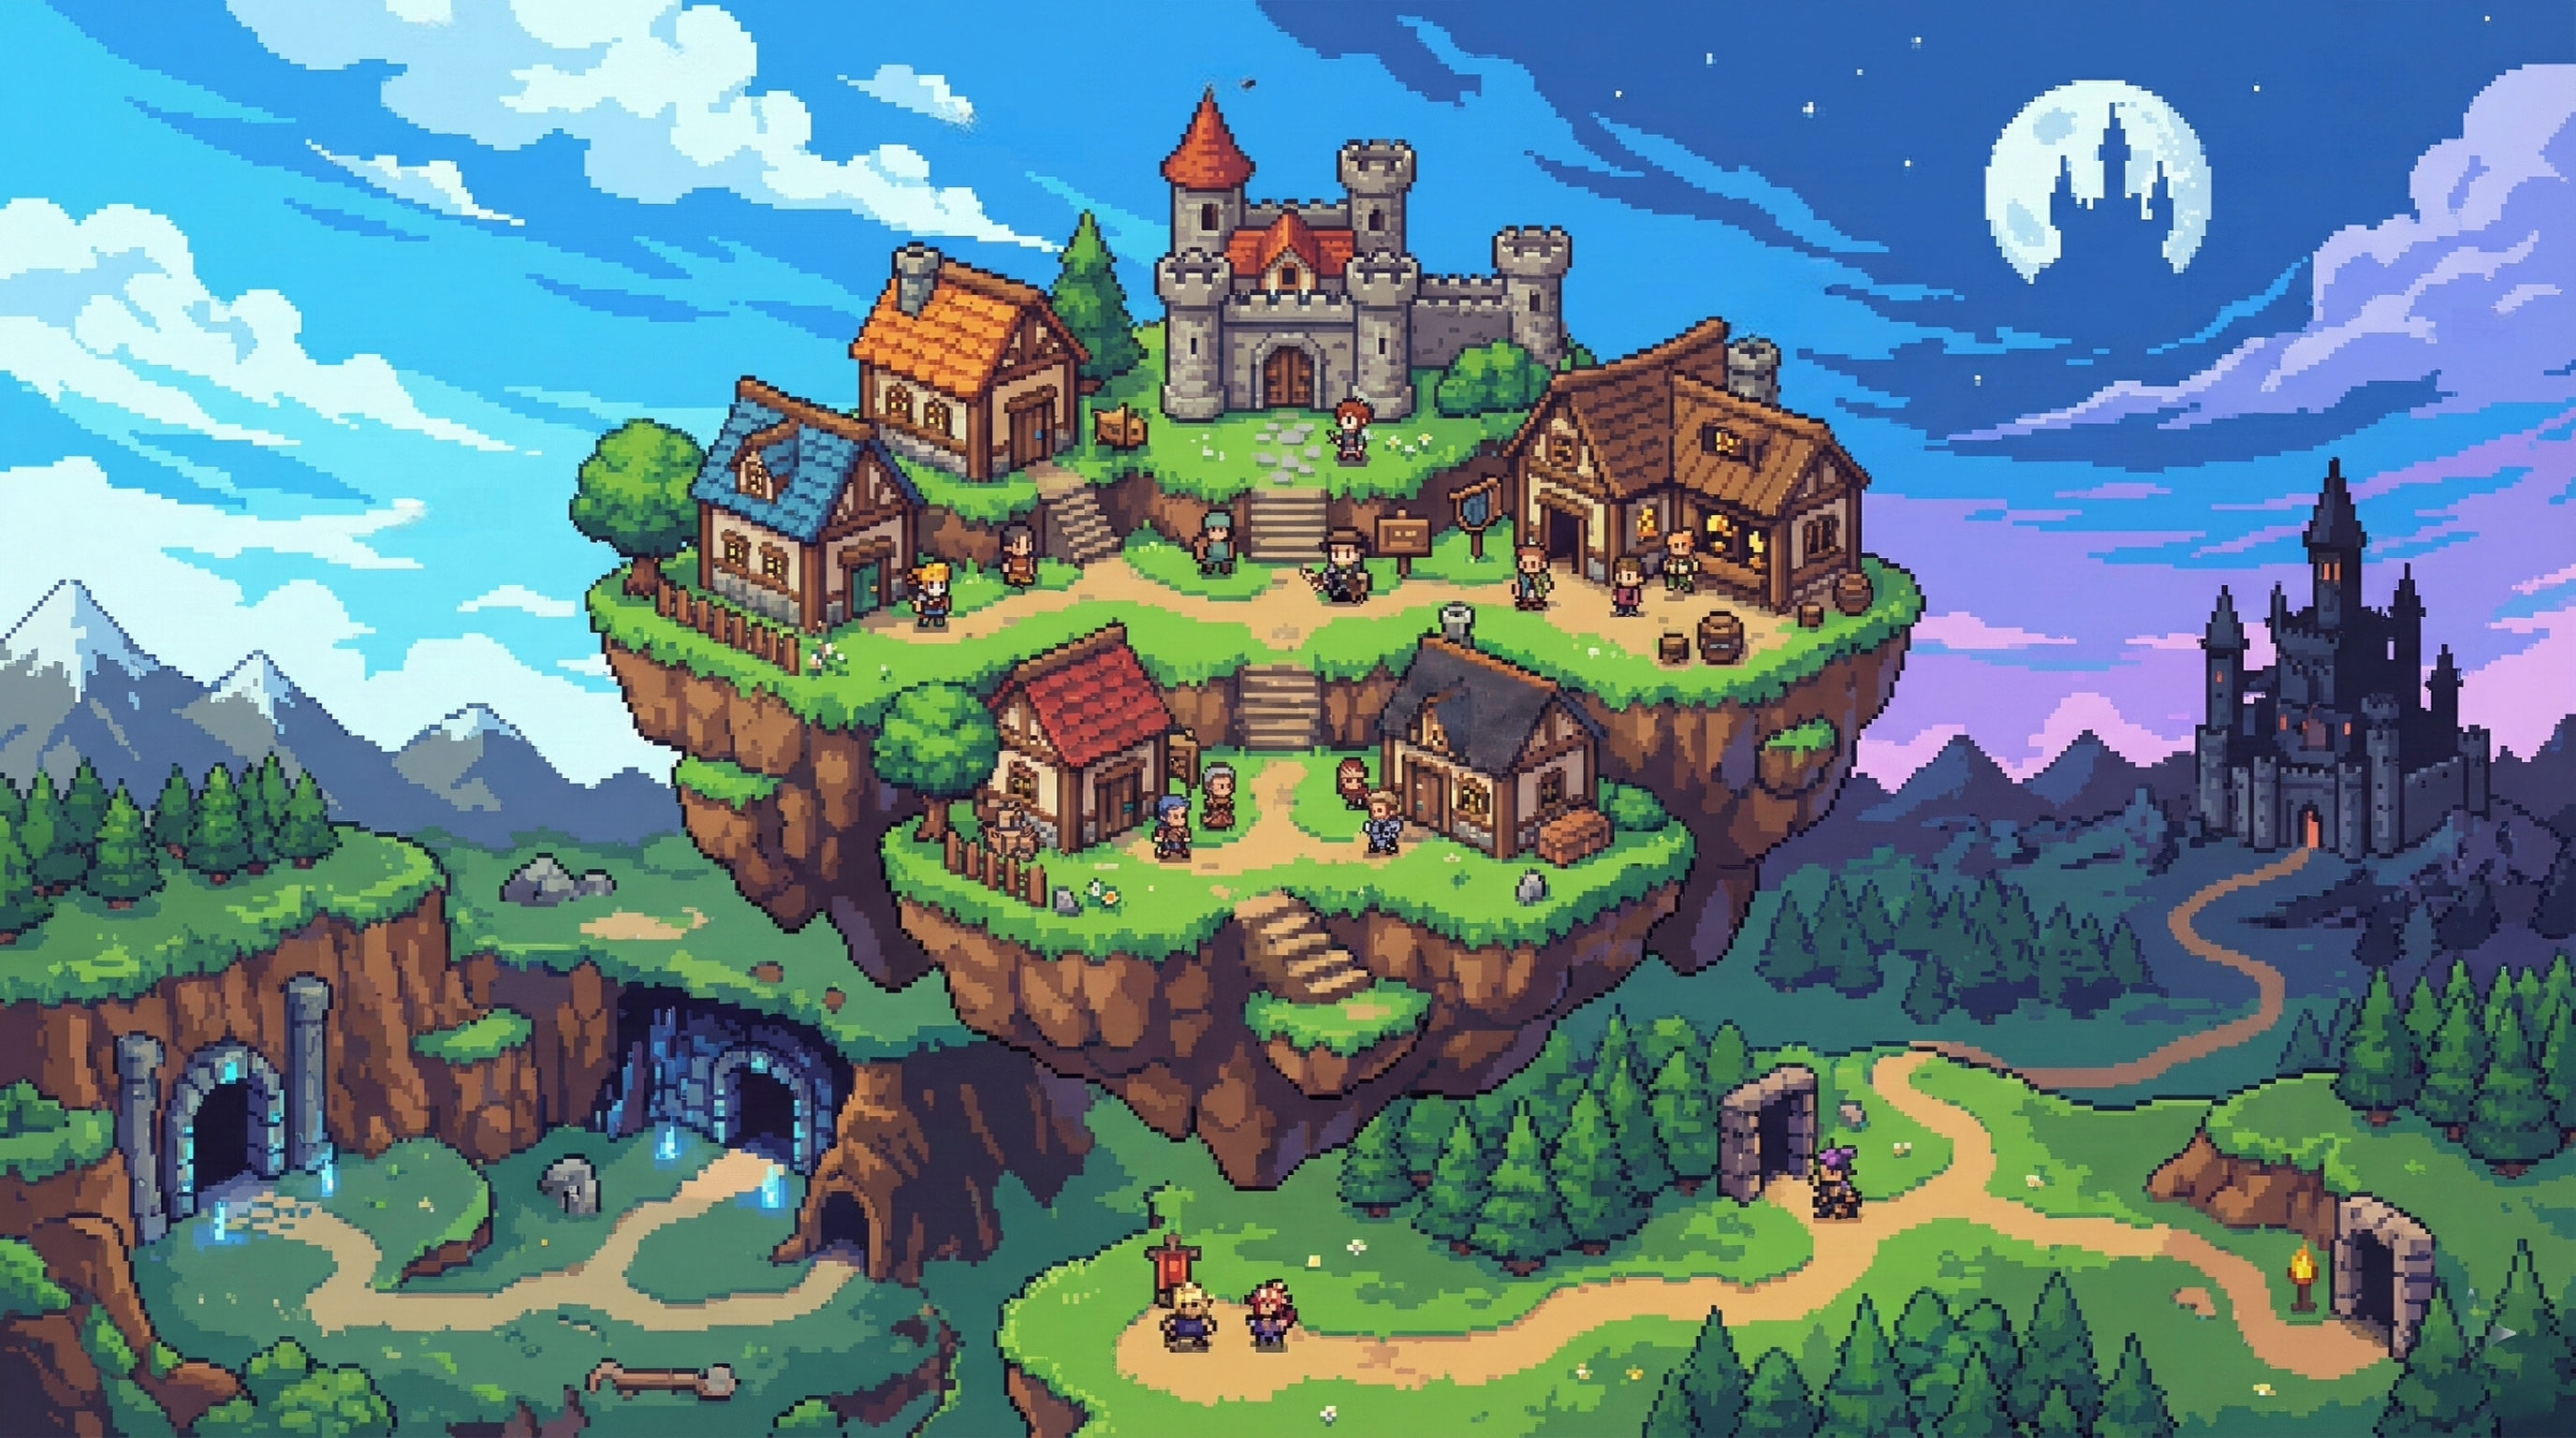
\includegraphics[width=\textwidth]{Images/background.png}
    \caption{Minh hoạ bối cảnh/\allowbreak pixel art mood của game}
    \label{fig:ui-background-mood}
\end{figure}

\subsubsection{Luồng UI xác thực: Login/\allowbreak Register}
\label{subsubsec:design-ui-auth}

\begin{figure}[H]
    \centering
    \includegraphics[width=0.78\textwidth]{Images/login.jpeg}
    \caption{Màn hình đăng nhập (Login)}
    \label{fig:ui-login}
\end{figure}

\begin{figure}[H]
    \centering
    \includegraphics[width=0.78\textwidth]{Images/register.jpeg}
    \caption{Màn hình đăng ký (Register)}
    \label{fig:ui-register}
\end{figure}

Mapping nghiệp vụ và API:
\begin{itemize}
    \item \textbf{Input validation}: username/\allowbreak password không rỗng; hiển thị lỗi theo mã lỗi chuẩn hoá.
    \item \textbf{Endpoint}: \texttt{/auth/\allowbreak login}, \texttt{/auth/\allowbreak register}; (tuỳ chọn) \texttt{/auth/\allowbreak recover}.
    \item \textbf{Trạng thái UI}: loading khi submit; disable nút khi request đang chạy; thông báo lỗi khi sai mật khẩu/\allowbreak tài khoản bị ban.
\end{itemize}

\subsubsection{Luồng UI profile: Select/\allowbreak Create/\allowbreak Delete}
\label{subsubsec:design-ui-profile}

\begin{figure}[H]
    \centering
    \includegraphics[width=0.95\textwidth]{Images/select_profile.png}
    \caption{Màn hình chọn profile (Select Profile)}
    \label{fig:ui-select-profile}
\end{figure}

\begin{figure}[H]
    \centering
    \includegraphics[width=0.95\textwidth]{Images/create_profile.png}
    \caption{Màn hình tạo profile/\allowbreak nhân vật (Create Profile/\allowbreak Character)}
    \label{fig:ui-create-profile}
\end{figure}

Mapping nghiệp vụ và API:
\begin{itemize}
    \item \textbf{Endpoint}: \texttt{/profiles} (list/\allowbreak create/\allowbreak select/\allowbreak delete), \texttt{/characters} (create/\allowbreak select/\allowbreak delete).
    \item \textbf{Ràng buộc}: giới hạn số profile/\allowbreak slot; xác nhận trước khi xoá; kiểm tra trùng tên theo policy.
    \item \textbf{Dữ liệu hiển thị}: level/\allowbreak class/\allowbreak race; thông tin preview ngoại hình lấy từ \texttt{CHARACTER.appearance}.
\end{itemize}

\subsubsection{UI Hub và điều hướng phân hệ}
\label{subsubsec:design-ui-hub}

\begin{figure}[H]
    \centering
    \includegraphics[width=\textwidth]{Images/main_UI.png}
    \caption{UI Hub: điều hướng Inventory/\allowbreak Heroes/\allowbreak Battle/\allowbreak Gacha/\allowbreak Quests}
    \label{fig:ui-main-hub}
\end{figure}

Mapping nghiệp vụ và API:
\begin{itemize}
    \item \textbf{Inventory}: REST tải \texttt{INVENTORY} + \texttt{CHARACTER\_EQUIPMENT} để render chỉ số và item/\allowbreak slot.
    \item \textbf{Heroes}: REST tải \texttt{NPC\_COLLECTION}.
    \item \textbf{Battle}: bắt đầu bằng REST (chuẩn bị data/\allowbreak kiểm tra điều kiện), sau đó chuyển sang WebSocket để realtime.
    \item \textbf{Gacha}: REST tải banner/\allowbreak rates, thực hiện summon, nhận kết quả và cập nhật NPC collection.
\end{itemize}

\subsubsection{UI Inventory/\allowbreak Equipment}
\label{subsubsec:design-ui-inventory}

\begin{figure}[H]
    \centering
    \includegraphics[width=\textwidth]{Images/inventory.jpg}
    \caption{UI Inventory: phân loại item, thao tác Use/\allowbreak Equip và hiển thị currency}
    \label{fig:ui-inventory}
\end{figure}

Mapping nghiệp vụ và API:
\begin{itemize}
    \item \textbf{Inventory tabs}: All/\allowbreak Equip/\allowbreak Use/\allowbreak Mat tương ứng filter theo \texttt{CONFIG\_ITEM.type}.
    \item \textbf{Endpoint}: \texttt{/inventory} (get/\allowbreak use), \texttt{/equipment} (get/\allowbreak equip/\allowbreak unequip), (tuỳ chọn) \texttt{/equipment/\allowbreak enhance}, \texttt{/equipment/\allowbreak repair}.
    \item \textbf{Ràng buộc}: kiểm tra slot trống; kiểm tra \texttt{max\_stack}; thao tác equip/\allowbreak unequip phải nhất quán giữa INVENTORY và CHARACTER\_EQUIPMENT.
\end{itemize}

% ==============================================================
\subsection{Thiết kế vòng lặp real-time cho combat/\allowbreak instance}
\label{subsec:design-realtime}

\subsubsection{Mô hình instance/\allowbreak room}
\label{subsubsec:design-room}

Hệ thống tổ chức người chơi theo \textbf{room} (đơn vị logic của một instance). Mỗi room có:
\begin{itemize}
    \item danh sách người chơi tham gia (socket id, character id);
    \item trạng thái runtime (vị trí, HP/\allowbreak MP, trạng thái skill, entity trong phòng);
    \item cấu hình phiên (mode: tower/\allowbreak dungeon/\allowbreak arena; floor/\allowbreak seed).
\end{itemize}

\subsubsection{Tick loop và phát snapshot}
\label{subsubsec:design-tick}

Thiết kế loop ở mức khái niệm:
\begin{enumerate}
    \item Thu thập input queue từ client.
    \item Xác thực input (cooldown, tài nguyên, vị trí hợp lệ, tốc độ).
    \item Cập nhật trạng thái authoritative theo tick.
    \item Phát snapshot định kỳ và phát event khi có thay đổi quan trọng (hit/\allowbreak loot/\allowbreak death).
\end{enumerate}

Trong giai đoạn 1, cơ chế snapshot có thể thiết kế theo hướng \textbf{đơn giản và rõ ràng}:
\begin{itemize}
    \item snapshot theo tick rate cố định (ví dụ 10--20 tick/\allowbreak s tuỳ mục tiêu kiểm thử);
    \item payload snapshot ưu tiên các giá trị tối thiểu để render (pos, hp/\allowbreak mp, state flags, cast state);
    \item chưa bắt buộc triển khai đầy đủ prediction/\allowbreak reconciliation, nhưng định dạng message chừa chỗ cho mở rộng \cite{gaffer-networking,moriarty-networked}.
\end{itemize}

% ==============================================================
\subsection{Thiết kế phân hệ Administration}
\label{subsec:design-admin}

Phân hệ admin phục vụ quản trị vận hành và kiểm soát rủi ro:
\begin{itemize}
    \item \textbf{Ban/\allowbreak Unban user}: cập nhật \texttt{USER.status}; thu hồi phiên đang hoạt động.
    \item \textbf{System mail}: gửi thông báo/\allowbreak phần thưởng theo user/\allowbreak profile; xử lý qua job để kiểm soát retry.
    \item \textbf{View logs}: truy vấn log theo thời gian/\allowbreak actor/\allowbreak severity; hỗ trợ điều tra sự cố.
    \item \textbf{Configure events/\allowbreak config}: quản trị cấu hình sự kiện và cấu hình gameplay theo phân quyền.
\end{itemize}

Các thao tác admin phải có:
\begin{itemize}
    \item phân quyền theo role;
    \item audit log đầy đủ (ai làm, làm gì, khi nào, trước/\allowbreak sau);
    \item cơ chế chống thao tác lặp gây cấp trùng phần thưởng (idempotent key).
\end{itemize}

% ==============================================================
\subsection{Bảo mật, nhất quán và quan sát hệ thống}
\label{subsec:design-nfr}

\subsubsection{Bảo mật}
\label{subsubsec:design-security}

Các nguyên tắc:
\begin{itemize}
    \item mật khẩu lưu dạng hash; không lưu plaintext;
    \item token có thời hạn; khi ban user cần thu hồi session;
    \item phân quyền rõ giữa player và admin (role-based);
    \item giới hạn tần suất login/\allowbreak gacha và kiểm tra input realtime để chống spam.
\end{itemize}

\subsubsection{Nhất quán dữ liệu và giao dịch nghiệp vụ}
\label{subsubsec:design-consistency}

Các thao tác như reward, gacha, exchange, equip/\allowbreak unequip, nâng cấp công trình/\allowbreak kỹ năng cần đảm bảo:
\begin{itemize}
    \item \textbf{atomic ở mức tài liệu} (MongoDB document update) khi cập nhật trong cùng thực thể;
    \item \textbf{idempotency} cho request dễ bị gửi lại (retry do mạng);
    \item \textbf{log nghiệp vụ} để có thể đối soát và khôi phục khi lỗi.
\end{itemize}

\subsubsection{Quan sát hệ thống (observability)}
\label{subsubsec:design-observability}

Thiết kế log tối thiểu:
\begin{itemize}
    \item request log: endpoint, latency, status code, user id (nếu có);
    \item business log: gacha result, reward delivery, currency delta, equip/\allowbreak skill-up actions, admin actions;
    \item realtime log: join/\allowbreak leave room, disconnect, lỗi xác thực socket.
\end{itemize}

% ==============================================================
\subsection{Tổng kết chương}
\label{subsec:design-summary}

Chương này đã mô tả thiết kế hệ thống ở mức kiến trúc, mô-đun, dữ liệu, giao tiếp và UI/\allowbreak UX tham chiếu cho \textit{Fortress of the Fallen}. Thiết kế nhấn mạnh ranh giới trách nhiệm client--server theo hướng server-authoritative, tổ chức backend theo mô-đun rõ ràng, tách dữ liệu tiến trình khỏi dữ liệu cấu hình, và xây dựng pipeline quản trị cấu hình theo hướng data-driven. Phần thiết kế dữ liệu đã cập nhật ERD (inventory/\allowbreak equipment/\allowbreak skills) và bổ sung data dictionary có caption để các bảng được đánh số và xuất hiện trong danh sách bảng. Các quyết định thiết kế này là nền tảng để mô tả hiện thực hệ thống và kiểm thử trong các chương tiếp theo \cite{nest-docs,mongodb-guide,redis-in-action,gaffer-networking,moriarty-networked}.

\section{Kế hoạch hiện thực prototype}
\label{sec:implementation}

\subsection{Mục tiêu và phạm vi}
\label{subsec:impl-goals}

Chương này mô tả kế hoạch hiện thực một \textbf{prototype} nhằm kiểm chứng các quyết định thiết kế đã trình bày ở Chương~\ref{sec:design}. Prototype được định hướng như một ``bản chạy được'' để xác thực:
\begin{itemize}
    \item Luồng \textbf{Identity \& Profile}: đăng ký/đăng nhập, chọn profile/nhân vật, thiết lập phiên.
    \item Luồng \textbf{real-time}: client gửi input, server xử lý authoritative và trả snapshot/event.
    \item Các mô-đun meta-progression có dữ liệu bền vững: \textbf{Inventory}, \textbf{Gacha}, \textbf{Personal Island \& NPC}.
    \item Pipeline \textbf{game configuration} theo hướng data-driven: Google Sheets $\rightarrow$ TSV $\rightarrow$ DB $\rightarrow$ Config Manager.
\end{itemize}

Trong phạm vi prototype, các nội dung (map, quái, AI phức tạp, PvP hoàn chỉnh) không phải trọng tâm; ưu tiên là \textbf{đúng luồng}, \textbf{đúng dữ liệu} và \textbf{đúng ranh giới client--server}.

%------------------------------------------------

\subsection{Kế hoạch triển khai theo mốc}
\label{subsec:impl-plan}

Kế hoạch triển khai được tổ chức theo các mốc tăng dần độ phức tạp: trước tiên dựng khung kết nối và xác thực, sau đó bổ sung hệ thống dữ liệu bền vững và cuối cùng là tích hợp các mô-đun meta.

\begin{table}[H]
\centering
\renewcommand{\arraystretch}{1.2}
\setlength{\tabcolsep}{6pt}
\begin{tabularx}{\textwidth}{|p{2.3cm}|X|p{4.2cm}|}
\hline
\textbf{Mốc} & \textbf{Mục tiêu kỹ thuật} & \textbf{Tính năng kiểm chứng} \\
\hline
M1 & Dựng backend, DB, auth và kết nối client & Register/Login, token, chọn profile \\
\hline
M2 & Dựng kênh real-time và room/instance runtime cơ bản & Join room, gửi input, nhận snapshot (di chuyển) \\
\hline
M3 & Tích hợp dữ liệu bền vững và mô-đun meta tối thiểu & Inventory/currency, gacha NPC, island resources, worker assignment \\
\hline
M4 & Hoàn thiện pipeline cấu hình và logging/audit tối thiểu & TSV import, config versioning, business logs \\
\hline
\end{tabularx}
\caption{Kế hoạch hiện thực prototype theo mốc}
\label{tab:impl-milestones}
\end{table}

%------------------------------------------------

\subsection{Hiện thực phía client (Unity)}
\label{subsec:impl-client}

\subsubsection{Tổ chức project và nguyên tắc phân lớp}
\label{subsubsec:impl-client-structure}

Client được tổ chức theo hướng tách biệt rõ ràng:
\begin{itemize}
    \item \textbf{Presentation/UI}: màn hình login, profile/character select, HUD cơ bản, panel inventory/gacha/island.
    \item \textbf{Gameplay}: điều khiển nhân vật, state machine animation, xử lý tương tác cơ bản.
    \item \textbf{Networking}: lớp HTTP client (REST) và WebSocket client (real-time), quản lý token, retry và timeout.
    \item \textbf{Data binding}: model dữ liệu để bind ra UI, tránh UI đọc trực tiếp dữ liệu thô từ network.
\end{itemize}

Nguyên tắc chính:
\begin{itemize}
    \item Client không tự ý ``xác nhận'' các thay đổi tiến trình (reward/currency/gacha).
    \item Client hiển thị trạng thái dựa trên phản hồi server; với realtime, ưu tiên snapshot/event authoritative.
\end{itemize}

\subsubsection{Luồng màn hình đề xuất}
\label{subsubsec:impl-client-flow}

Luồng điều hướng UI tối thiểu cho prototype:
\begin{enumerate}
    \item \textbf{Login/Register}: nhập thông tin, gọi API, lưu token.
    \item \textbf{Profile Select}: liệt kê profile, tạo/chọn profile.
    \item \textbf{Character Select/Create}: liệt kê nhân vật theo profile, tạo/chọn nhân vật.
    \item \textbf{Main Hub (Island)}: load scene, hiển thị HUD, mở các panel inventory/gacha/NPC/island.
    \item \textbf{Join Instance (tuỳ mốc)}: tham gia room realtime để kiểm chứng đồng bộ di chuyển/combat đơn giản.
\end{enumerate}

\subsubsection{Networking client: REST + WebSocket}
\label{subsubsec:impl-client-network}

Client duy trì 2 kênh:
\begin{itemize}
    \item \textbf{REST}: các thao tác quản lý (auth/profile/character/inventory/island/gacha).
    \item \textbf{WebSocket}: join room, gửi input, nhận snapshot/event.
\end{itemize}

Quy ước xử lý lỗi UI:
\begin{itemize}
    \item \textbf{401/403}: token hết hạn hoặc sai quyền $\rightarrow$ điều hướng về login.
    \item \textbf{5xx}: lỗi hệ thống $\rightarrow$ hiển thị trạng thái retry.
    \item \textbf{network timeout}: hiển thị offline/reconnect và không cho thao tác tiến trình.
\end{itemize}

%------------------------------------------------

\subsection{Hiện thực phía server (NestJS)}
\label{subsec:impl-server}

\subsubsection{Cấu trúc module và luồng request}
\label{subsubsec:impl-server-modules}

Backend triển khai theo module hoá để bám sát ranh giới nghiệp vụ:
\begin{itemize}
    \item \textbf{AuthModule}: register/login, issue token, guard/role.
    \item \textbf{ProfileModule}: CRUD profile, chọn profile, cập nhật last\_played.
    \item \textbf{CharacterModule}: CRUD character, load character summary.
    \item \textbf{InventoryModule}: get inventory, apply delta (reward, currency), equip/enhance (tuỳ mốc).
    \item \textbf{GachaModule}: banner/rate/summon, update pity, duplicate handling.
    \item \textbf{IslandModule}: get island, build/upgrade, resource sync.
    \item \textbf{NpcModule}: list NPC, assign worker, update job state.
    \item \textbf{RealtimeGateway}: websocket auth, join room, input handling, snapshot broadcasting.
    \item \textbf{ConfigModule}: load config collections, provide lookup service, expose config version.
\end{itemize}

Luồng xử lý chuẩn cho REST:
\begin{enumerate}
    \item Guard xác thực token và gắn context (userId/profileId/characterId nếu có).
    \item Validate DTO và kiểm tra ràng buộc nghiệp vụ.
    \item Thực hiện cập nhật DB theo hướng atomic ở mức tài liệu (document update).
    \item Ghi business log/audit log nếu là giao dịch quan trọng.
\end{enumerate}

\subsubsection{Realtime: room runtime và tick loop tối thiểu}
\label{subsubsec:impl-server-realtime}

Room runtime được lưu trong bộ nhớ server (in-memory) trong phạm vi prototype:
\begin{itemize}
    \item \texttt{roomId}, \texttt{mode} (island/tower/dungeon/arena), danh sách player trong room.
    \item Runtime state: position, HP/MP, flags trạng thái, cooldown state tối thiểu.
    \item Input queue theo socket.
\end{itemize}

Tick loop tối thiểu (không tối ưu hoá) theo các bước:
\begin{enumerate}
    \item Nhận input và đưa vào queue theo \texttt{seq}.
    \item Validate input (rate limit, trạng thái hợp lệ, không vượt tốc độ).
    \item Cập nhật state và tạo snapshot.
    \item Broadcast snapshot theo nhịp (tick rate cấu hình).
\end{enumerate}

Trong mốc đầu, snapshot chỉ cần chứa thông tin đủ để render:
\[
\{\;entityId,\;pos,\;rot,\;hp,\;mp,\;stateFlags\;\}
\]
Các kỹ thuật nâng cao (prediction/reconciliation) được xem là hướng mở rộng sau khi luồng cơ bản ổn định.

%------------------------------------------------

\subsection{Thiết kế hiện thực dữ liệu và truy xuất}
\label{subsec:impl-data}

\subsubsection{Schema collections và nguyên tắc embed/reference}
\label{subsubsec:impl-data-schema}

Các collections động (progression/state) ưu tiên embed khi dữ liệu gắn chặt vòng đời:
\begin{itemize}
    \item \textbf{CHARACTER}: nhúng base\_stats/resources/position/appearance.
    \item \textbf{INVENTORY}: nhúng danh sách item instance.
    \item \textbf{PERSONAL\_ISLAND}: nhúng island resources và danh sách buildings.
    \item \textbf{NPC\_COLLECTION}: nhúng danh sách owned NPC.
\end{itemize}

Các collections cấu hình (static) dùng reference qua khoá \texttt{id}:
\begin{itemize}
    \item \textbf{CONFIG\_ITEM}: định nghĩa item.
    \item \textbf{CONFIG\_BUILDING}: định nghĩa building và cost/time.
    \item (mở rộng) \textbf{CONFIG\_SKILL}, \textbf{CONFIG\_RATES}, \textbf{CONFIG\_FORMULAS}, \ldots
\end{itemize}

\subsubsection{Nguyên tắc cập nhật an toàn cho giao dịch tiến trình}
\label{subsubsec:impl-data-safety}

Các thao tác nhạy cảm (reward/currency/gacha/build upgrade) cần:
\begin{itemize}
    \item \textbf{Idempotency key}: mỗi request có mã định danh giao dịch để tránh cấp trùng khi retry.
    \item \textbf{Business log}: ghi lại delta trước/sau (hoặc sự kiện) để đối soát.
    \item \textbf{Atomic update}: với dữ liệu trong một document, ưu tiên update trong một thao tác DB.
\end{itemize}

%------------------------------------------------

\subsection{Hiện thực pipeline game configuration}
\label{subsec:impl-config}

\subsubsection{Định dạng TSV và quy ước}
\label{subsubsec:impl-config-tsv}

Mỗi TSV đại diện một bảng cấu hình, có cột \texttt{id} làm khoá chính. Quy ước:
\begin{itemize}
    \item Header dòng đầu tiên; encoding UTF-8.
    \item Kiểu dữ liệu rõ ràng (int/float/string/bool) theo template.
    \item Các tham chiếu chéo dùng khoá \texttt{id} (ví dụ itemRefId, buildingId).
\end{itemize}

\subsubsection{Import script: upsert và log phiên bản}
\label{subsubsec:impl-config-import}

Script import thực hiện:
\begin{enumerate}
    \item Parse TSV theo schema (validate required fields, type).
    \item Upsert theo \texttt{id} vào collection tương ứng.
    \item Tạo bản ghi \texttt{CONFIG\_IMPORT\_LOG} gồm: thời gian import, bảng, số dòng, checksum, người thực hiện.
    \item Cập nhật \texttt{config\_version} (tăng dần) để runtime biết phiên bản đang chạy.
\end{enumerate}

\subsubsection{Config Manager runtime}
\label{subsubsec:impl-config-manager}

Config Manager nạp dữ liệu cấu hình từ DB vào bộ nhớ khi server khởi động:
\begin{itemize}
    \item Lưu theo map: \texttt{(tableName, id) $\rightarrow$ object}.
    \item Cung cấp API nội bộ: \texttt{getItem(id)}, \texttt{getBuilding(id)}, \texttt{getFormula(key)}.
    \item Khi trả dữ liệu về client, có thể kèm \texttt{config\_version} để debug nhất quán.
\end{itemize}

%------------------------------------------------

\subsection{Kế hoạch kiểm thử và tiêu chí nghiệm thu}
\label{subsec:impl-testing}

\subsubsection{Kiểm thử theo use case}
\label{subsubsec:impl-uc-test}

Kiểm thử ưu tiên theo các use case trọng yếu (Chương~\ref{sec:analysis}):
\begin{itemize}
    \item Auth: register/login, token expiry.
    \item Profile/Character: create/select, load summary.
    \item Realtime: join room, move input, snapshot update, disconnect handling.
    \item Gacha: summon 1x/10x, pity update, duplicate handling, history.
    \item Island/NPC: build/upgrade timer (mock), assign worker, resource tick (mô phỏng).
\end{itemize}

\subsubsection{Kiểm thử dữ liệu và tính nhất quán}
\label{subsubsec:impl-consistency-test}

Các kịch bản cần kiểm chứng:
\begin{itemize}
    \item Retry request (gacha/reward) không làm nhân đôi kết quả.
    \item Inventory stack và slot không vượt giới hạn.
    \item Worker assignment không tạo trạng thái treo (NPC vừa ``rảnh'' vừa ``đang làm'').
    \item Import TSV sai schema bị từ chối và không làm ``bẩn'' config.
\end{itemize}

\subsubsection{Tiêu chí nghiệm thu prototype}
\label{subsubsec:impl-acceptance}

Prototype đạt yêu cầu khi thoả tối thiểu:
\begin{itemize}
    \item Có thể đăng nhập, chọn profile/nhân vật và vào scene hub.
    \item Có thể tham gia room realtime và đồng bộ di chuyển ổn định.
    \item Gacha trả kết quả hợp lệ, lưu DB, cập nhật pity và xử lý trùng lặp.
    \item Island/NPC có luồng dữ liệu bền vững (lưu và tải lại đúng).
    \item Pipeline TSV import tạo được config version và runtime truy xuất đúng theo version.
\end{itemize}

%------------------------------------------------

\subsection{Tổng kết chương}
\label{subsec:impl-summary}

Chương này đã trình bày kế hoạch hiện thực prototype nhằm kiểm chứng thiết kế hệ thống: tổ chức client và server, luồng REST/WebSocket, room realtime tối thiểu, chiến lược lưu trữ dữ liệu, pipeline game configuration theo TSV và kế hoạch kiểm thử theo use case. Kết quả của chương là cơ sở để thực hiện đánh giá/đối chiếu trong chương tiếp theo khi prototype được triển khai và chạy thử.

\section{Đánh giá hệ thống}
\label{sec:evaluation}

\subsection{Mục tiêu và phương pháp đánh giá}
\label{subsec:eval-method}

Mục tiêu của chương này là đánh giá mức độ phù hợp của bản thiết kế hệ thống (Chương~\ref{sec:design}) so với yêu cầu đã phân tích (Chương~\ref{sec:requirements}), đồng thời chỉ ra các điểm mạnh, hạn chế và rủi ro còn tồn tại. Do giai đoạn 1 tập trung vào thiết kế, phương pháp đánh giá được thực hiện theo các hướng:
\begin{itemize}
    \item \textbf{Đối chiếu bao phủ yêu cầu (Requirement Coverage)}: kiểm tra các yêu cầu chức năng/phi chức năng đã được ánh xạ tới mô-đun, dữ liệu và luồng giao tiếp hay chưa.
    \item \textbf{Đánh giá kiến trúc theo thuộc tính chất lượng (Quality Attributes)}: nhất quán dữ liệu, bảo mật, khả năng mở rộng, tính bảo trì, khả năng quan sát.
    \item \textbf{Đánh giá tính khả thi triển khai (Feasibility)}: dựa trên kế hoạch prototype ở Chương~\ref{sec:implementation} và các kịch bản use case trọng yếu ở Chương~\ref{sec:analysis}.
    \item \textbf{Phân tích rủi ro và hướng giảm thiểu}: xác định các rủi ro kỹ thuật/thiết kế, mức ảnh hưởng và biện pháp kiểm soát.
\end{itemize}

\subsection{Đối chiếu bao phủ yêu cầu chức năng}
\label{subsec:eval-functional}

\subsubsection{Ma trận bao phủ yêu cầu theo mô-đun}
\label{subsubsec:eval-functional-matrix}

Bảng~\ref{tab:req-coverage} tổng hợp ánh xạ giữa các nhóm yêu cầu chức năng (FR) và mô-đun thiết kế ở Chương~\ref{sec:design}. Mục tiêu là đảm bảo mọi nhóm yêu cầu đều có ``điểm đặt'' rõ ràng trong kiến trúc.

\begin{table}[H]
\centering
\renewcommand{\arraystretch}{1.2}
\setlength{\tabcolsep}{6pt}
\begin{tabularx}{\textwidth}{|p{2.6cm}|p{4.1cm}|X|}
\hline
\textbf{Nhóm FR} & \textbf{Phân hệ} & \textbf{Mô-đun/Thiết kế đáp ứng} \\
\hline
FR-A & Auth \& Profile & AuthModule, ProfileModule, SessionRuntime (token, profile\_id, socket\_id) \\
\hline
FR-B & Character & CharacterModule (create/select/delete), dữ liệu nhúng appearance/base\_stats/resources \\
\hline
FR-C & Stats/Level/Slots & CharacterModule + ConfigModule (milestone slots, công thức chỉ số data-driven) \\
\hline
FR-D & Class System & CharacterModule/Progression service (unlock/switch), điều kiện theo stat/trait/achievement \\
\hline
FR-E & Inventory/Economy & InventoryModule (stack, capacity, currency, equip/enhance), tham chiếu CONFIG\_ITEM \\
\hline
FR-F & Combat/Modes & CombatModule + RealtimeGateway (join instance, tick, snapshot, end-session reward/checkpoint) \\
\hline
FR-G & Gacha & GachaModule (banner/rate/pity/duplicate/history), NPC\_COLLECTION cập nhật bền vững \\
\hline
FR-H & Island \& NPC & IslandModule (build/upgrade/timer/resources), NpcModule (assign worker, job state) \\
\hline
FR-I & Admin & AdminModule (ban/unban, mail, logs, event config), audit log \\
\hline
\end{tabularx}
\caption{Ma trận bao phủ yêu cầu chức năng theo mô-đun}
\label{tab:req-coverage}
\end{table}

Kết quả đối chiếu cho thấy các nhóm tính năng chính đều đã được gắn với mô-đun và dữ liệu tương ứng, phù hợp hướng module hoá theo phân hệ của backend \cite{nest-docs}.

\subsubsection{Đánh giá luồng nghiệp vụ trọng yếu}
\label{subsubsec:eval-critical-flows}

Các luồng nghiệp vụ được xem là trọng yếu vì ảnh hưởng trực tiếp tới tiến trình hoặc tính công bằng:

\paragraph{(1) Auth $\rightarrow$ Profile $\rightarrow$ Character $\rightarrow$ Session}
Luồng này có trạng thái phụ thuộc theo chuỗi (USER $\rightarrow$ GAME\_PROFILE $\rightarrow$ CHARACTER) và có yêu cầu nhất quán ở session runtime. Thiết kế đáp ứng bằng:
\begin{itemize}
    \item REST dùng để xác thực và chọn profile/character;
    \item session runtime lưu \texttt{profile\_id}/\texttt{character\_id} để WebSocket có thể xác định bối cảnh phiên;
    \item token có hạn và có thể revoke khi cần (ban/unban).
\end{itemize}

\paragraph{(2) Reward delivery và cập nhật inventory}
Luồng thưởng sau phiên (tower/dungeon) dễ phát sinh lỗi cấp trùng nếu người chơi retry hoặc mất kết nối. Thiết kế giảm rủi ro bằng:
\begin{itemize}
    \item server-authoritative: client không tự ghi reward;
    \item cập nhật inventory theo quy tắc stack/capacity và tham chiếu config item;
    \item đề xuất idempotency và business log để đối soát.
\end{itemize}

\paragraph{(3) Gacha: rate/pity/duplicate}
Luồng gacha có yêu cầu “đúng xác suất theo cấu hình” và “không cấp trùng”. Thiết kế đáp ứng bằng:
\begin{itemize}
    \item rates/banners là game configuration (tĩnh) và có thể quản trị bằng pipeline;
    \item pity là state (động) lưu bền vững theo banner hoặc nhóm banner;
    \item duplicate handling chuyển đổi theo rule, giảm cảm giác ``mất giá trị''.
\end{itemize}

\paragraph{(4) Island build/upgrade và worker assignment}
Luồng island có rủi ro trạng thái treo (worker vừa rảnh vừa bận, hoặc building có worker nhưng worker không trỏ về building). Thiết kế đáp ứng bằng:
\begin{itemize}
    \item cập nhật liên kết hai chiều khi assign worker;
    \item timer (\texttt{finish\_time}) và trạng thái building rõ ràng;
    \item island/resources và buildings nhúng trong cùng thực thể để truy xuất nhất quán.
\end{itemize}

\subsection{Đánh giá yêu cầu phi chức năng}
\label{subsec:eval-nfr}

\subsubsection{Bảo mật và phân quyền}
\label{subsubsec:eval-security}

Thiết kế đáp ứng các yêu cầu bảo mật nền tảng:
\begin{itemize}
    \item mật khẩu lưu hash (không plaintext);
    \item token có thời hạn; WebSocket handshake phải xác thực token;
    \item phân quyền admin theo role; thao tác admin có audit log;
    \item giới hạn tần suất thao tác nhạy cảm (login/gacha) và kiểm soát spam input realtime.
\end{itemize}
Hướng tiếp cận này phù hợp nguyên tắc hệ thống online: hạn chế tin tưởng client và đặt kiểm tra luật ở server \cite{moriarty-networked}.

\subsubsection{Nhất quán dữ liệu và khả năng chống cấp trùng}
\label{subsubsec:eval-consistency}

Đối với game online, nhất quán dữ liệu quan trọng hơn tối ưu sớm. Thiết kế thể hiện các điểm tích cực:
\begin{itemize}
    \item tách rõ dữ liệu động và tĩnh; dữ liệu tĩnh được nạp qua Config Manager để đồng bộ cách tính;
    \item cập nhật tiến trình (inventory/gacha/island) định hướng atomic ở mức document;
    \item đề xuất idempotency key cho các giao dịch dễ retry (reward/gacha/build upgrade).
\end{itemize}

Hạn chế còn lại: ở mức thiết kế, cơ chế idempotency và transaction log mới dừng ở nguyên tắc, chưa có đặc tả schema log/delta chi tiết cho từng giao dịch. Đây là phần cần đặc tả thêm khi chuyển sang hiện thực.

\subsubsection{Hiệu năng và khả năng mở rộng}
\label{subsubsec:eval-performance}

Thiết kế ưu tiên chạy ổn định ở mức đồ án, nhưng vẫn có hướng mở rộng:
\begin{itemize}
    \item realtime tách riêng bằng WebSocket gateway và mô hình room runtime in-memory để giảm độ trễ;
    \item Redis được định hướng dùng cho cache/pub-sub khi scale ngang nhiều instance;
    \item Config Manager nạp config vào bộ nhớ giúp giảm truy vấn DB cho dữ liệu tĩnh.
\end{itemize}

Hạn chế:
\begin{itemize}
    \item room runtime in-memory khiến việc scale ngang cần thêm cơ chế phân vùng room (room sharding) hoặc session affinity;
    \item chưa có tiêu chí tick-rate/bandwidth cụ thể theo mục tiêu tải.
\end{itemize}
Các hạn chế này phù hợp với phạm vi giai đoạn 1 (thiết kế), và sẽ được xử lý khi nâng mức triển khai/benchmark.

\subsubsection{Tính bảo trì và khả năng mở rộng tính năng}
\label{subsubsec:eval-maintainability}

Tính bảo trì được hỗ trợ bởi:
\begin{itemize}
    \item module hoá theo phân hệ rõ ràng (Auth/Profile/Character/Inventory/Combat/Gacha/Island/Admin);
    \item cross-cutting service cho validation, error handling, logging;
    \item cấu hình data-driven giúp thay đổi nội dung/thông số mà không sửa code lõi.
\end{itemize}

Điểm cần chú ý: khi số lượng phân hệ tăng, cần kiểm soát phụ thuộc chéo (đặc biệt giữa Progression/Inventory/Gacha) bằng cách chuẩn hoá service interface và event nội bộ.

\subsubsection{Khả năng quan sát (Observability)}
\label{subsubsec:eval-observability}

Thiết kế đã nêu các lớp log tối thiểu:
\begin{itemize}
    \item request log (latency/status/user context);
    \item business log (reward/currency/gacha/admin actions);
    \item realtime log (join/leave room/disconnect).
\end{itemize}

Đánh giá: hướng này đủ cho giai đoạn prototype và debug nghiệp vụ. Để nâng lên vận hành thực tế, cần bổ sung thêm metric (tick time, snapshot size, error rate), tracing và cảnh báo.

\subsection{Đánh giá pipeline cấu hình game (data-driven config)}
\label{subsec:eval-config}

Pipeline cấu hình: Google Sheets $\rightarrow$ TSV $\rightarrow$ DB $\rightarrow$ Config Manager, chỉ áp dụng cho \textbf{game configuration}.

\subsubsection{Ưu điểm}
\begin{itemize}
    \item \textbf{Giảm hard-code}: các thông số (item/building/rate/formula) được thay đổi qua TSV.
    \item \textbf{Dễ kiểm soát phiên bản}: TSV có thể quản lý qua version control; import log giúp truy vết.
    \item \textbf{Tối ưu truy xuất runtime}: Config Manager nạp in-memory, phù hợp với các phép tra cứu thường xuyên.
\end{itemize}

\subsubsection{Rủi ro và kiểm soát}
\begin{itemize}
    \item \textbf{Sai schema/kiểu dữ liệu}: cần validation khi import và báo lỗi rõ ràng theo dòng/cột.
    \item \textbf{Tham chiếu chéo sai}: cần kiểm tra referential integrity (itemRefId/buildingId/skillId).
    \item \textbf{Không đồng bộ phiên bản giữa instance}: nếu chạy nhiều server, cần cơ chế reload đồng bộ hoặc restart theo chiến lược triển khai.
\end{itemize}

\subsection{Đánh giá UI/UX theo định hướng pixel art ở mức hệ thống}
\label{subsec:eval-ui}

Do UI theo phong cách pixel art nhấn mạnh readability và phản hồi nhanh, thiết kế hệ thống hỗ trợ UX bằng:
\begin{itemize}
    \item chuẩn hoá trạng thái UI (loading/error/disabled) thông qua mã lỗi nhất quán;
    \item ưu tiên payload ``delta'' hoặc snapshot nhỏ gọn cho HUD combat;
    \item phân tách màn hình meta (inventory/gacha/island) khỏi HUD combat để không làm gián đoạn nhịp chơi.
\end{itemize}

Hạn chế: chưa có đặc tả UI state machine chi tiết cho từng màn (ví dụ: trường hợp disconnect khi đang ở gacha hoặc đang xây building). Đây là phần có thể mở rộng ở giai đoạn hiện thực prototype.

\subsection{Phân tích rủi ro và hướng giảm thiểu}
\label{subsec:eval-risks}

Bảng~\ref{tab:risk-register} liệt kê các rủi ro kỹ thuật chính và hướng giảm thiểu trong phạm vi đồ án.

\begin{table}[H]
\centering
\renewcommand{\arraystretch}{1.2}
\setlength{\tabcolsep}{6pt}
\begin{tabularx}{\textwidth}{|p{3.3cm}|p{2.0cm}|X|p{4.2cm}|}
\hline
\textbf{Rủi ro} & \textbf{Mức} & \textbf{Mô tả} & \textbf{Giảm thiểu} \\
\hline
Cấp trùng reward/gacha & Cao &
Retry do mạng/mất kết nối có thể tạo giao dịch lặp &
Idempotency key, business log, kiểm thử retry, chốt trạng thái bằng server-authoritative \\
\hline
Trạng thái treo worker assignment & Trung bình &
NPC và building lệch trạng thái (một chiều) &
Cập nhật hai chiều, validate trước khi assign/unassign, kịch bản kiểm thử nhất quán \\
\hline
Sai config gây mất cân bằng/lỗi runtime & Cao &
TSV sai kiểu hoặc tham chiếu chéo sai gây crash hoặc lệch gameplay &
Validation import, schema strict, referential checks, config version + rollback \\
\hline
Realtime latency/jitter làm mất cảm giác combat & Trung bình &
Snapshot không ổn định gây giật/khó điều khiển &
Tick-rate hợp lý, snapshot tối thiểu, client interpolation; chừa chỗ mở rộng prediction/reconciliation \\
\hline
Phụ thuộc chéo giữa mô-đun tăng dần & Trung bình &
Feature mới kéo theo gọi chéo nhiều service khó bảo trì &
Chuẩn hoá interface, domain services rõ ràng, event nội bộ, review dependency định kỳ \\
\hline
\end{tabularx}
\caption{Bảng rủi ro và hướng giảm thiểu}
\label{tab:risk-register}
\end{table}

\subsection{Tổng kết chương}
\label{subsec:eval-summary}

Kết quả đánh giá cho thấy bản thiết kế đã:
\begin{itemize}
    \item bao phủ các nhóm yêu cầu chức năng chính thông qua mô-đun hoá rõ ràng và mô hình dữ liệu nhất quán;
    \item đáp ứng các yêu cầu phi chức năng nền tảng (bảo mật, nhất quán, bảo trì, quan sát) ở mức phù hợp với phạm vi giai đoạn 1;
    \item đưa ra pipeline quản trị game configuration theo hướng data-driven, giúp giảm phụ thuộc vào hard-code và tạo nền tảng cân bằng nội dung.
\end{itemize}

Các điểm còn cần đặc tả sâu hơn khi chuyển sang hiện thực gồm: cơ chế idempotency/log cho từng giao dịch, chính sách xử lý overflow inventory, tiêu chí tick-rate/bandwidth cho realtime và đặc tả UI state chi tiết cho các tình huống lỗi mạng.

\section{Kết luận và hướng phát triển}
\label{sec:conclusion}

\subsection{Tổng kết kết quả đạt được}
\label{subsec:conclusion-summary}

Đồ án \textit{Fortress of the Fallen} được xây dựng theo định hướng một game Action RPG online với lớp meta-progression phong phú, kết hợp nhiều mô-đun gameplay: tiến trình leo tháp (tower), chiến đấu theo phiên (instance), quản lý nhân vật và chỉ số, gacha tuyển dụng thực thể dài hạn (NPC), và hệ thống đảo cá nhân theo hướng base-building.

Trong phạm vi giai đoạn 1 tập trung vào \textbf{thiết kế hệ thống}, báo cáo đã đạt được các kết quả chính:
\begin{itemize}
    \item \textbf{Xác định yêu cầu và phạm vi}: hệ thống hoá các yêu cầu chức năng theo phân hệ (auth/profile, character/progression, inventory/economy, combat, gacha, island \& NPC, admin) và các yêu cầu phi chức năng (bảo mật, nhất quán, mở rộng, quan sát).
    \item \textbf{Phân tích hệ thống theo use case và luồng nghiệp vụ}: mô tả tác nhân, use case tổng quan và đặc tả các luồng trọng yếu (đăng nhập--chọn profile, tạo nhân vật, reward delivery, gacha, island build/upgrade và worker assignment).
    \item \textbf{Thiết kế kiến trúc client--server}: phân tách rõ REST cho thao tác quản lý và WebSocket cho realtime; áp dụng nguyên tắc server-authoritative cho các thao tác ảnh hưởng tiến trình.
    \item \textbf{Thiết kế dữ liệu}: tổ chức thực thể lõi (USER, GAME\_PROFILE, CHARACTER, INVENTORY, PERSONAL\_ISLAND, NPC\_COLLECTION, SESSION\_RUNTIME), chỉ ra quan hệ và nguyên tắc embed/reference phù hợp cho MongoDB.
    \item \textbf{Thiết kế pipeline game configuration theo hướng data-driven}: Google Sheets $\rightarrow$ TSV $\rightarrow$ DB $\rightarrow$ Config Manager (chỉ áp dụng cho các bảng cấu hình/thông số gameplay), giúp giảm hard-code và hỗ trợ quản trị phiên bản cấu hình.
    \item \textbf{Kế hoạch hiện thực prototype và đánh giá thiết kế}: đề xuất các mốc triển khai để kiểm chứng thiết kế và đánh giá mức độ bao phủ yêu cầu, chất lượng kiến trúc, rủi ro và biện pháp giảm thiểu.
\end{itemize}

\subsection{Đóng góp của đồ án}
\label{subsec:conclusion-contributions}

Các đóng góp chính của đồ án trong phạm vi thiết kế bao gồm:
\begin{itemize}
    \item \textbf{Bộ khung thiết kế hệ thống hoàn chỉnh cho một game online theo mô-đun}, có thể mở rộng theo nhiều hướng (thêm nội dung, mở rộng server, bổ sung dịch vụ phụ trợ).
    \item \textbf{Mô hình dữ liệu bền vững và nhất quán} phục vụ các mô-đun meta-progression (inventory, gacha, island \& NPC) đồng thời giữ được ranh giới rõ ràng giữa dữ liệu động (progress) và dữ liệu tĩnh (config).
    \item \textbf{Định hướng giao tiếp realtime có khả năng phát triển}: thiết kế envelope message và vòng đời phiên (handshake, join room, input, snapshot/event, end session), tạo nền cho việc bổ sung các kỹ thuật networking nâng cao.
    \item \textbf{Pipeline cấu hình game độc lập với dữ liệu tiến trình}, giúp nhóm nội dung có thể điều chỉnh cân bằng và mở rộng nội dung mà không phụ thuộc nhiều vào thay đổi mã nguồn.
\end{itemize}

\subsection{Hạn chế}
\label{subsec:conclusion-limitations}

Do tập trung vào giai đoạn 1 (thiết kế), một số nội dung chưa được hiện thực hoặc chưa được kiểm chứng bằng benchmark:
\begin{itemize}
    \item \textbf{Cơ chế giao dịch nghiệp vụ chi tiết}: idempotency/log/delta cho từng loại giao dịch (reward, gacha, upgrade) mới dừng ở mức nguyên tắc; cần đặc tả schema log và quy trình đối soát cụ thể hơn khi hiện thực.
    \item \textbf{Realtime nâng cao}: thiết kế đã chừa chỗ cho mở rộng, nhưng chưa triển khai và đánh giá các kỹ thuật như prediction/reconciliation, interest management và tối ưu băng thông.
    \item \textbf{Chính sách xử lý ngoại lệ}: các trường hợp đặc thù như overflow inventory, reconnect giữa phiên, rollback khi import config lỗi cần được đặc tả sâu và kiểm thử khi prototype chạy thật.
    \item \textbf{Đánh giá hiệu năng theo tải}: chưa có số đo thực nghiệm cho tick time, snapshot size, throughput hoặc độ ổn định khi tăng số lượng kết nối.
\end{itemize}

\subsection{Hướng phát triển}
\label{subsec:conclusion-future}

Trong các giai đoạn tiếp theo, hệ thống có thể phát triển theo các hướng ưu tiên sau:

\subsubsection{Hiện thực prototype và kiểm chứng theo use case}
\begin{itemize}
    \item Hoàn thiện prototype theo các mốc đã đề xuất: auth/profile, realtime room, meta modules (inventory/gacha/island), pipeline config.
    \item Xây dựng bộ kiểm thử theo kịch bản: retry giao dịch, mất kết nối, đồng bộ dữ liệu sau reconnect, consistency giữa NPC và building.
\end{itemize}

\subsubsection{Nâng cấp realtime cho cảm giác chiến đấu}
\begin{itemize}
    \item Bổ sung interpolation chuẩn cho client và phân tách snapshot/event rõ ràng.
    \item Thử nghiệm prediction/reconciliation cho chuyển động cơ bản, sau đó mở rộng cho kỹ năng.
    \item Tối ưu payload snapshot (delta compression) và áp dụng interest management khi có nhiều thực thể trong room.
\end{itemize}

\subsubsection{Hoàn thiện hệ thống giao dịch và chống gian lận}
\begin{itemize}
    \item Chuẩn hoá idempotency key cho các endpoint nhạy cảm (reward/gacha/upgrade).
    \item Thiết kế business ledger (sổ giao dịch) để truy vết thay đổi currency và phần thưởng theo thời gian.
    \item Tăng cường kiểm soát input realtime (anti-spam/anti-speedhack) dựa trên luật server-authoritative.
\end{itemize}

\subsubsection{Mở rộng pipeline cấu hình}
\begin{itemize}
    \item Mở rộng nhóm config: skill definitions, drop tables, banner schedules, formulas và economy sinks/sources.
    \item Bổ sung kiểm tra tham chiếu chéo và cơ chế rollback phiên bản khi import gây lỗi.
    \item Khi chạy nhiều instance server: đồng bộ reload config bằng pub/sub hoặc chiến lược triển khai có kiểm soát phiên bản.
\end{itemize}

\subsubsection{Chuẩn hoá quan sát hệ thống}
\begin{itemize}
    \item Bổ sung metrics (tick time, snapshot size, error rate), tracing theo request/correlation id.
    \item Chuẩn hoá log nghiệp vụ cho các thao tác quan trọng và dashboard quan sát cho admin.
\end{itemize}

\subsection{Kết luận}
\label{subsec:conclusion-final}

Báo cáo đã trình bày đầy đủ quá trình từ xác định bài toán, phân tích yêu cầu, phân tích hệ thống đến thiết kế kiến trúc, dữ liệu và kế hoạch hiện thực prototype cho \textit{Fortress of the Fallen}. Các quyết định thiết kế tập trung vào tính mô-đun, tính nhất quán dữ liệu và hướng data-driven cho cấu hình gameplay, tạo nền tảng vững để triển khai prototype và mở rộng hệ thống trong các giai đoạn tiếp theo.


% ===================== TIMELINE GIAI ĐOẠN TIẾP THEO =====================
% Nếu bạn muốn timeline nằm trong Phụ lục thì chuyển \input này sang Content/appendices.
\clearpage
% ===================== Content/contributions.tex =====================
\clearpage
\section*{Phân công nhiệm vụ và đóng góp của các thành viên}
\addcontentsline{toc}{section}{Phân công nhiệm vụ và đóng góp của các thành viên}

Phần này tổng hợp phạm vi công việc và mức đóng góp của từng thành viên trong suốt quá trình thực hiện đồ án. Việc phân công được xây dựng dựa trên thế mạnh của mỗi thành viên và được phối hợp xuyên suốt theo từng mốc triển khai, nhằm đảm bảo tính nhất quán giữa trải nghiệm người dùng (client/UI) và xử lý nghiệp vụ (server/DB/giao tiếp).

\renewcommand{\arraystretch}{1.25}
\setlength{\tabcolsep}{6pt}

\begin{table}[H]
\centering
\begin{tabularx}{\textwidth}{|p{3.2cm}|X|p{3.2cm}|p{3.0cm}|}
\hline
\textbf{Hạng mục} & \textbf{Mô tả công việc} & \textbf{Thành viên chính} & \textbf{Phối hợp} \\
\hline
Lên ý tưởng đề tài & Thống nhất định hướng gameplay, scope hệ thống, các phân hệ chính (auth, profile/character, inventory/equipment, skills, island/npc, combat/gacha). & Toàn + Khang & Cả hai \\
\hline
Tìm game tham khảo và chốt hướng UI & Tìm các tựa game/reference phù hợp, tổng hợp luồng UI, bố cục màn hình và quy ước tương tác để chốt phong cách giao diện và trải nghiệm. & Hà Thái Toàn & Trần Minh Khang \\
\hline
Client và UI/UX & Thiết kế luồng màn hình (login/register, profile, create character, main hub, inventory), định nghĩa UI state (loading/error/disabled), chuẩn hoá dữ liệu hiển thị theo response từ API. & Hà Thái Toàn & Trần Minh Khang \\
\hline
Đề xuất tính năng và đánh giá khả thi & Đề xuất các tính năng trọng tâm theo phạm vi đồ án; đánh giá rủi ro/độ phức tạp; chốt các chức năng phải server-authoritative và các điểm cần audit/log. & Trần Minh Khang & Hà Thái Toàn \\
\hline
Hiện thực hệ thống server & Thiết kế/hiện thực backend theo mô-đun; tổ chức REST API và WebSocket; xác thực, phân quyền, xử lý lỗi; chuẩn hoá payload; quản lý session runtime và luồng nghiệp vụ chính. & Trần Minh Khang & Hà Thái Toàn \\
\hline
Đồng bộ client--server & Thống nhất contract dữ liệu giữa UI và API (endpoint, request/response, message envelope realtime), rà soát mismatch, điều chỉnh luồng để đảm bảo trải nghiệm mượt và dữ liệu nhất quán. & Cả hai & Cả hai \\
\hline
\end{tabularx}
\caption{Phân công nhiệm vụ và đóng góp của các thành viên}
\label{tab:team-contributions}
\end{table}

\clearpage

\clearpage
% ===================== Content/timeline_next_phase.tex =====================
\section*{Kế hoạch giai đoạn tiếp theo}
\addcontentsline{toc}{section}{Kế hoạch giai đoạn tiếp theo}

Phần này trình bày kế hoạch triển khai cho giai đoạn sau khi hoàn tất giai đoạn thiết kế (Giai đoạn 1). Timeline dưới đây mang tính định hướng theo tuần, có thể điều chỉnh theo mức độ hoàn thiện thực tế và phạm vi nghiệm thu.

\renewcommand{\arraystretch}{1.2}
\begin{table}[H]
\centering
\setlength{\tabcolsep}{6pt}
\begin{tabularx}{\textwidth}{|p{2.2cm}|X|p{4.2cm}|}
\hline
\textbf{Mốc} & \textbf{Hạng mục thực hiện} & \textbf{Kết quả/Deliverables} \\
\hline
Tuần 1 & Chuẩn hoá project Unity + NestJS; thiết lập pipeline build cơ bản; chuẩn hoá cấu trúc module; tạo seed DB và import config (TSV) & Repo ổn định; script import TSV; Config Manager nạp được config \\
\hline
Tuần 2 & Hoàn thiện Identity/Profile/Character: đăng ký/đăng nhập; tạo/chọn profile; tạo/chọn nhân vật; đồng bộ dữ liệu vào DB & API hoàn chỉnh; luồng đăng nhập $\rightarrow$ chọn profile $\rightarrow$ chọn nhân vật chạy được \\
\hline
Tuần 3 & Inventory \& Equipment: slot/stack; currency; trang bị theo slot; cập nhật derived stats theo equipment & CRUD inventory/equipment; validate ràng buộc; payload ổn định cho UI \\
\hline
Tuần 4 & Skill Module: học kỹ năng; skill points; hotbar; validate cooldown/mana cost theo config & CharacterSkills hoạt động; hotbar mapping; test luồng học + gán phím \\
\hline
Tuần 5 & Gacha \& NPC Collection: banner/rate; lưu lịch sử; duplicate handling; cập nhật NPC collection & Endpoint gacha + lưu kết quả; nhật ký gacha; mô hình NPC collection chạy được \\
\hline
Tuần 6 & Island Module: tài nguyên; xây/nâng cấp; timer; gán worker; validate layout grid & Luồng xây/upgrade; worker assignment; cập nhật resources \\
\hline
Tuần 7 & Realtime skeleton: WebSocket gateway; join room; gửi input; snapshot tối thiểu; test độ trễ cơ bản & Room loop chạy; message envelope; snapshot ổn định (prototype) \\
\hline
Tuần 8 & Tích hợp + kiểm thử: test tích hợp theo use-case; kiểm thử dữ liệu; hardening lỗi; log/audit; viết tài liệu triển khai & Báo cáo test; checklist luồng nghiệp vụ; log/audit cho reward/gacha/admin \\
\hline
\end{tabularx}
\caption{Timeline triển khai giai đoạn tiếp theo (định hướng theo tuần)}
\label{tab:next-phase-timeline}
\end{table}

\noindent
\textbf{Ghi chú vận hành:}
\begin{itemize}
    \item Các mốc có thể chạy song song theo phân hệ, nhưng cần ưu tiên hoàn tất pipeline config và luồng đăng nhập/profile/character trước để tạo nền cho các module còn lại.
    \item Với các phần realtime, giai đoạn đầu ưu tiên chạy được loop và snapshot tối thiểu; các kỹ thuật nâng cao (prediction/reconciliation) chỉ bổ sung khi đủ thời gian.
\end{itemize}


% ===================== TÀI LIỆU THAM KHẢO =====================
\clearpage
\addcontentsline{toc}{section}{Tài liệu tham khảo}
\printbibliography

% ===================== PHỤ LỤC =====================
\clearpage
\input{Content/appendices}

\end{document}
